\documentclass[12pt, a4paper]{article}
\usepackage{url,graphicx,tabularx,array,geometry}
\usepackage[utf8]{inputenc}
\usepackage{paralist}
\usepackage{latexsym}
\usepackage{ upgreek }
\usepackage{fancyhdr}
\usepackage{ textcomp }
\usepackage{ mathrsfs }
\usepackage{cancel}

\pagestyle{fancy}

\usepackage{amsmath}
\usepackage{amsfonts}
\usepackage{amssymb}
\usepackage{arydshln}
\usepackage{listings}

\DeclareUnicodeCharacter{00A0}{ }

\setlength{\parskip}{1ex} %--skip lines between paragraphs
\setlength{\parindent}{0pt} %--don't indent paragraphs

%-- Commands for header
\newcommand{\bs}{\ensuremath{\backslash}}
\renewcommand{\title}[1]{\textbf{#1}\\}
\renewcommand{\line}{\begin{tabularx}{\textwidth}{X>{\raggedleft}X}\hline\\\end{tabularx}\\[-0.5cm]}
\newcommand{\leftright}[2]{\begin{tabularx}{\textwidth}{X>{\raggedleft}X}#1%
& #2\\\end{tabularx}\\[-0.5cm]}
%\linespread{2} %-- Uncomment for Double Space
\begin{document}
\renewcommand{\headrulewidth}{0pt}
\fancyhf{}
\fancyhead[L]{
\leftright{}{Daniel Schmidt}
\line
\leftright{\textbf{DBT SS 16 - VL}}{}}
\fancyfoot[C]{\thepage}

\section*{Deduktive Datenbanksysteme}

\textbf{Problem:} Transitiver Abschluss ist in PL1 nicht formulierbar (mit zustandsabhängiger Formulierung möglich)\\
\textbf{Diskussion:} \\
Typ 5: $q_1(...), ..., q_n(...) :- .$\\
Typ 6: $q_1(...),...,q_n(...) :- p_1(...),...,p_m(...).$\\
$\Rightarrow$ Übungsaufgabe

Nur Typ 1 und Typ 4: $q(...) :- p_1(...),...,p_n(...), n \ge 0$ (ist die Hornklauselform und wird bei definiten Datenbanken genutzt) 

\subsection*{Definite Datenbanken}
\begin{equation}
\begin{split}
q(...) &:- . \text{(Fakt)}\\
q(...) &:- p_1(...),...,p_n(...). \text{(deduktive Regel, } p_{1-n} \text{ Teilziele)}
\end{split}
\end{equation}

\begin{itemize}
\item Mit IBen (Integritätsbedingungen) (+ Typ2, Typ3) ($:- p_1(...), ...,p_n(...)$)
\item Typ5 + Typ6 $\Rightarrow$ \textbf{Disjunktive Datenbank}
\item Definite Datenbank + negative Atome im Rumpf von Hornklauseln erlaubt $\Rightarrow$ Volles Datalog
\end{itemize}

\subsubsection*{Formulierung von Anfragen}
Klauseln vom Typ: $:- p_1(...),....,p_n(...)$, geschrieben $? - p_1(...),....,p_n(...)$

Beispiele:
\begin{itemize}
\item $? - ag(X,m).$
\begin{itemize}
\item Bedeutung: Welche Kurse bietet 'm' an?
\item DRC: (x) / ANGEBOT(X, m) 
\end{itemize}
\item $? - ag(a3,m).$
\begin{itemize}
\item Bedeutung: Bietet 'm' den Kurs 'a3' an?
\item DRC: () / ANGEBOT(a3, m) 
\end{itemize}
\item $? - ag(X,m), bl(X,s,j).$
\begin{itemize}
\item Bedeutung: Gib alle von 'm' angebotene Kurse, die 's' als Wiederholer belegt hat
\item DRC: (x) / ANGEBOT(x, 'm') $\wedge$ BELEGUNG(x, 's', 'y') 
\end{itemize}
\item Wie ist (x) / ANGEBOT(x, 'm') $\wedge (\exists $y) BELEGUNG(x, 's', y) formulierbar?
\begin{itemize}
\item Bedeutung: Gib die Dozenten der von s als Wiederholer belegte Kurse
\item Formulierung: $? - Ksm(X). \\ Ksm(X) :- ag(X, m), bl(X,s,y)$
\item Bequemer: $?- ag(X, Y*), bl(X,s,y).$, * Kennzeichnet die Ausgabevariable
\end{itemize}
\end{itemize}

In Anfragesprachen werden Vergleichsausdrücke benötigt. Dazu sind in Datalog spezielle vordefinierte Prädikate vorhanden. Für jeden Vergleichsoperator wird die Existenz eines solchen Prädikates angenommen.\\
Zunächst: Beschränkte Variablen in Regeln. Sei eine Regel r gegeben:
\begin{itemize}
\item Jede Variable, die als Argument in einem gewöhnlichen Prädikat im Rumpf von r vorkommt ist beschränkt.
\item Jede Variable, die in einem Teilziel $X=c$ oder $c=X$ von r vorkommt, ist beschränkt.
\item Eine Variable X ist beschränkt, wenn sie in einem Teilziel $X=Y$ oder $Y=X$ von r vorkommt mit Y ist schon als beschränkt bekannt.
\end{itemize}

\subsubsection*{Definition: sicher}
Eine Regel heißt sicher, wenn alle in ihr vorkommenden Variablen beschränkt sind.

\paragraph*{Beispiele:}
\begin{itemize}
\item $Kls(X,Y) :- bl(Z, s, j), ag(Z, Y), X=Z.$ \textbf{sicher}
\item $vsj(X,Y) :- bl(Y,s,j).$ \textbf{nicht sicher} (X ist nicht beschränkt)
\item $vs(X,Y) :- vs(X, Z), kp(Z, Y).$ \textbf{sicher, wenn vs terminiert}
\item $kla(Z,Y) :- bl(Z,V,j), ag(Z,Y), V \neq s.$ \textbf{sicher}
\end{itemize}

\paragraph*{Bemerkung:} Falls keine Build-in Prädikate erlaubt sind (/vorkommen):\\
Eine Regel ist sicher genau dann wenn jede Variable im Kopf der Regel auch im Rumpf der Regel vorkommt.

\subsubsection*{Definition: Datalog Programm}
Ein Datalog-Programm P (ohne IBen(Integritätsbedingungen)) ist eine endliche Menge von Horn-Klauseln mit Jedes $d \in P$ ist entweder
\begin{itemize}
\item ein Fakt $q(...).$ ohne Variable
\item eine sichere Regel $q(...) :- p_1(...),...,p_n(...).$ mit $q\in iPraedikat$
\end{itemize}

Ein $d \in P$ heißt auch \textbf{Datalog-Klausel}
Alle Fakten zu extensionalen Prädikaten sind als in DB-Relationen gespeichert zu denken.

\paragraph*{Beispiel}
Datenbankzustand:

\begin{equation}
\begin{split}
&ag(a1, m).\\
&kp(c2, a0).\\
&... \\
&rb(a1, r1, t1) \textit{(Kurs a1 im Raum r1 zu t1)}\\
&rb(a3,r2,t4)
\end{split}
\end{equation}

Angebot: \\
\begin{tabular}{|c|c|}
\hline
Kursnummer & Dozent\\ \hline
a1 & m \\
... & ... \\
\hline
\end{tabular}

Kursplan: \\
\begin{tabular}{|c|c|}
\hline
Kursnummer & Voraussetzung\\ \hline
c2 & a0 \\
... & ... \\
\hline
\end{tabular}

Raumbelegung: \\
\begin{tabular}{|c|c|c|}
\hline
Kursnummer & Raum & Zeit\\ \hline
a1 & r1 & t1 \\
... & ... \\ & ... \\
\hline
\end{tabular}

Belegung: \\
\begin{tabular}{|c|c|c|}
\hline
Kursnummer & Teilnehmer & Wiederholer\\ \hline
a1 & s & j \\
... & ... \\ & ... \\
\hline
\end{tabular}

\begin{equation}
\begin{split}
vs(X, Y) &:- Kp(X,Y). \\
vs(X, Y) &:- vs(X, Z), Kp(Z, Y). \\
stdpl(W,X,Y,Z) &:- bl(X, W, V), rb(X,Y,Z). \\
ueberschneidungen(X,Y) &:- Kp(Z, X), Kp(Z, Y), rb(X, V,T), rb(Y, W, T), X \neq Y.
\end{split}
\end{equation}


\subsubsection*{Deklarative Semantik}
Extensionale Prädikate eines Programms (ext. Rel, ext. DB): EDB\\
Intentionale Prädikate eines Programms (int. Rel, int. DB): IDB\\

\paragraph*{Bedeutung}
Bedeutung eines Datalog-Programms P: Menge derjenigen Grundatome zu den intentionalen Prädikaten von P, die logisch aus P gefolgert werden können. (Jedes Modell von P ist auch ein Modell von $f \in F$). Mit Zielklausel g(...), $g \in Praed$: Aus P logisch folgerbare Grundatome zu g, die von g(..) subsummiert (überdeckt) werden.
\begin{tabular}{c}
g(a,X) \\ \hline
g(a,b) \\
g(a,c)
\end{tabular}

In P werden Werte aus Wertebereichen verwendet, ebenso in Darstellung der extensionalen Prädikate als DB-Relation. Daher können wir $Kost_A$ und Dom idefntifizieren. Mithilfer der Herbrand Interpretation kann die Semantik festgelegt werden (ist möglich).


\paragraph*{Herbrand-Interpretation /-Modelle}

Gewöhnliche Interpretation: \\
\begin{equation}
\begin{split}
Konst_A &= \{ a,b \}, Dom = \{ \circ, \square \} \\
k(a) &= \circ\\
k(b) &= \square \\
ext(p(.,.)) &=  \{ (\circ, \square), (\square, \square) 
\end{split}
\end{equation}

eine mögliche Herbrand-Interpretation (passt dazu)
\begin{equation}
\begin{split}
Konst_A &= Dom = \{ a,b \} \\
k(a) &= a\\
k(b) &= b \\
ext(p(.,.)) &=  \{ (a, b), (b, b) 
\end{split}
\end{equation}

Entsprechende Herbrand-Interpretation. Betrachte alle Paare zu p(.,.), teste gemäß gegebener (gewöhnlicher) Interpretationin ext(p(.,.)).
\begin{equation}
\begin{split}
Konst_A &= \{ a,b \}, Dom = \{ \circ, \square \} \\
k(a) &= \square\\
k(b) &= \square \\
ext(p(.,.)) &=  \{ (\circ, \square), (\square, \square) 
\end{split}
\end{equation}
(a,a) wird zu $(\square, \square) \in ext(p(.,.))$

Herbrand-Interpretation
\begin{equation}
\begin{split}
Konst_A &= Dom = \{ a,b \} \\
k(a) &= a\\
k(b) &= b \\
ext(p(.,.)) &=  \{ (a,a), (a, b), (b,a), (b,b) \}
\end{split}
\end{equation}

Bei beiden Interpretationen sind die gleichen Formeln gültig bei Beschränkung auf quantorenfreie Formeln ohne Variablen (und ohne Funktionen).

\paragraph*{Beispiel}

Erste Interpretation: $p(a,b) \wedge p(b,a) \Rightarrow (\square, \square) \in ext(p(.,.)) \wedge ...$ bzw. $(a,b) \in ext(p(.,.)) \wedge (b,a) \in ext(p(.,.))$

Menge von Konstanten und Prädikatensymbole ist endlich, daher ist die Anzahl der möglichen Herbrand-Interpreationen endlich.

\subsubsection*{Satz von Gödel / Skolem (Herbrand, 1930)}
Eine Klauselmenge P hat ein Modell genau dann wenn P hat ein Herbrand-Modell.
Daraus folgt, dass ein Verfahren analog zu Wahrheitstabellen in der Aussagenlogik möglich ist.

\paragraph*{Beispiel}
$F = \{ p(a) \Rightarrow q(b), p(a) \wedge q(b) \}$, $q(b)?$

\begin{tabular}{|c|c|c|c|c|}
\hline
p & q & $p(a) \Rightarrow q(b) \text{erfüllt?}$ & $p(a) \wedge q(b) \text{erfüllt?}$ & $p(a) \Rightarrow q(b) \text{und} p(a) \wedge q(b) \text{erfüllt?}$\\ \hline
$\{\}$ & $\{\}$ & \checkmark & - & - \\
$\{\}$ & $\{ a \}$ & \checkmark & - & - \\
$\{\}$ & $\{ b \}$ & \checkmark & \checkmark & \checkmark \\
$\{\}$ & $\{ a, b \}$ & \checkmark & \checkmark & \checkmark \\
$\{ a \}$ & $\{\}$ & - & \checkmark & - \\
... & ... & ... & ... & .... \\
$\{ b \}$ & $\{ b \}$ & \checkmark & \checkmark & \checkmark
\end{tabular}

Jedes Modell von F ist auch ein Modell von q(b), d.h. q(b) kann aus F logisch gefolgert werden. Gilt bei Klauselmengen, aber \textbf{Vorsicht bei allgemeinen Formeln}.
\paragraph*{Beispiel:} $\{p(a), (\exists X) (\lnot p(X))\}$ Formelmenge, keine Klauselmenge

Modell (vgl. Übung): 
\begin{equation}
\begin{split}
Dom &= \{ 0, 1 \} \\
k(a) &= 0\\
ext(p(.)) &=  \{ (0) \} 
\end{split}
\end{equation}

\paragraph*{Aber:} Es gibt kein durch \texttt{ext} bestimmtes Herbrand-Modell:

\begin{enumerate}
\item $ext(p(.)) = \{(a)\}, Konst = Dom = \{ a \}$
\item $ext(p(.) = \{\})$
\end{enumerate}

Herbrand-Modell muss genügend viele Elemente enthalten, damit der Satz von Gödel / Skolem gelten kann. \textbf{Skolemisierung} bedeutet, dass man alle Existenzquantoren durch Funktionen ersetzt:

\begin{equation}
(\forall X_1,....,X_n)(\exists y) (F) \leadsto (\forall X_1,...,X_n)(F[f(X_1,...X_n) / y])
\end{equation}


\subsubsection*{Bemerkung: Skolemisierung}

Jede Formel der PL1 Logik kann man in einer \underline{erfüllbarkeitsäquivalente} Formel in Skolemform umformen:
\begin{enumerate}
\item Pränexnormalform
\item Umformungen à la $(\forall X_1,....,X_n)(\exists y) (F) \leadsto (\forall X_1,...,X_n)(F[f(X_1,...X_n) / y])$ mit jeweils einem neuen Funktionssymbol
\end{enumerate}
Dies ist eine Art ``Materialisierung'' der durch den Existenzquantor gebundenen Variablen.

\paragraph*{Beispiel (von oben)}

$\{p(a), \lnot p(y)\footnote{neue Variable} \}$ erfüllbar $\Longleftrightarrow \{p(a), (\exists X)(\lnot p(X))\}$ erfüllbar \\

\textbf{Vorsicht:} Semantische Äquivalenz von Formeln und ihren Skolem-Normalformen im Allgemeinen bicht gegeben.

Skolem-NF: $(\exists X)(p(X)) : p(a)$
Interpretation I mit 
\begin{equation}
\begin{split}
Dom &= \{ 1, 2 \} \\
k(a) &= 1\\
ext(p(.)) &=  \{ (2) \} 
\end{split}
\end{equation}

$\leadsto \vDash_I (\exists X)(p(X))$
Belegung von X mit allen Elementen aus Dom, d.h. auch mit 2. Aber $\not \vDash_I p(a)$, da $(1) \not \in ext(p(.))$.

\subsubsection*{Im Kontext von Datalog}
\begin{itemize}
\item Herbrand-Universum: Konst
\item Herbrand-Basis (HB): Menge aller Grundatome \\ ($\leadsto EDB\footnote{gegeben durch Datenbankzustand}, IDB\footnote{muss ausgerechnet / gefolgert werden} \text{(Fakten in der Datenbank und solche die Ableitbar sind)} \subset HB$ )
\item Herbrand-Interpretation: (Konst, id, ext), d.h. jedes Konstantensymbol wird als es selbst interpretiert. (Verglichen mit relationaler Interpretation, dort $k$ ist Bijektion)
\item Jede Herbrand-Interpretation ist eindeutig bestimmt durch $ext$ (Extension, Ausprägung), da Konst und id unveränderlich sind
\item Jedes Prädikat ist eindeutig bestimmt durch die Angabe der Grundatome, für  die es ``wahr'' liefert.
\item extentional: genaue Antwort in Tupel
\item intentional: Beispielsweise Formeln als Antworten
\end{itemize}

\subsubsection*{Definition: Herbrand-Interpretation}
Einfache Definition: Eine Herbrand-Interpretation ist eine Teilmenge der Herbrand-Basis.


\paragraph*{Beispiel Kursverwaltung}

\begin{equation}
\begin{split}
\text{Aus DB-Rel. KURSPLAN} &\leadsto kp \in ePr\ddot{a}d \\
vs(X,Y) :- kp(X,Y) &\leadsto vs \in iPr\ddot{a}d
\end{split}
\end{equation}

\paragraph*{Gesucht:} Durch Programm P bestimmte Grundatome (Fakten).

\subsubsection*{Definition: Grundatom}
Ein Grundatom f ist eine logische Folgerung einer Menge D von Datalog Klauseln (z.B. $D \vDash f$) $\diamondsuit_{Def}$. Jedes Herbrand Modell von D ist auch ein Modell von f.\\
Da f ein Grundatom ist gilt $D \vDash f \Longrightarrow f $ ist in jedem Herbrand-Modell von D enthalten. Das heißt $f \in \bigcap \{ I | I Herbrand-Modell von D \}$.\\
Sei $f \in \bigcap \{ I | I Herbrand-Modell von D \}$, dann ist f ein Grundatom und jedes Modell von D auch in Modell von f. 

\subsubsection*{Definition: Mege aller Konsequenzen}

$cons(D) =_{def} \{ f \in HB_D | D \vDash f \}$


\subsection*{Satz 1.1}

$cons(D) = \bigcap \{ I | I Herbrand-Modell von D \}$ \\
Aufgrund der Eigenschaften unserer Regel ist der Schnitt / cons(D) ein Modell, dies gilt es zu beweisen: \\

Da $cons(D) \subseteq HB_D$, ist $cons(D)$ eine Herbrand-Interpretation.

\subsection*{Satz 1.2} 

$cons(D)$ ist ein Herbrand-Modell von D.

\subsubsection*{Beweis}
\paragraph*{z.Z.} 
Jedes $d \in D$ ist gültig in dieser Interpretation, also $cons(D)$ ($\vDash_{cons(D)} d$).

\paragraph*{Beweis}

Falls $d$ ein Grundatom ist gehört $d$ zu jedem Herbrandmodell von D, daraus folgt $d \in cons(D)$. \\
Sei d eine Regel $q(...) :- p_1(...),...,p_m(...)$. Sei $\varrho$ eine Belegung für die Variable von d. \textit{Annahme:} $(\forall 1 \le i \le m)(|| p_i(.)||^{\varrho} \in cons(D))$, sonst d gültig unter $cons(D)$.
Für jedes Herbrand-Modell I von D gilt, dann $||p_i(.)||^{\varrho} \in I, i = 1, ..., m$ und damit $||q_(.)||^{\varrho} \in cons(D),$ da $d$ eine Horn-Klausel ist.
(Der Schluss ist z.B. für $d = q_1(...), q_2(...) :- p_1(...), ..., p_n(...)$ nicht möglich.) \\

Damit $D \vDash_{cons(D)} ||q(...)||^{\varrho} \in cons(D)$. Wir erhalten, dass $cons(D)$ ein Herbrand-Modell von D ist. Da $d$ beliebig gewählt wird folgt der Satz.

$cons(D)$ ist offensichtlich eindutig bestimmt und das kleinste Herbrand-Modell von D. Damit: Seantik eines Datalog-Programms P ist gegeben durch das kleinste Herbrand-Modell von P oder (äquivalent) durch $cons(P) = \{ f\in HB_{P} | O \vDash f \}$.

\paragraph*{Beispiel}
$r \in ePr\ddot{a}d, p,q \in iPr\ddot{a}d, Konst = \{ 1, 2, 3 \}$.

\textbf{Fakten}: \\
\begin{equation}
\begin{split}
r(1).& \\
p(X) &:- q(X). \\
q(X) &:- r(X).
\end{split}
\end{equation}

\textbf{Herbrand-Modelle}: \\
\begin{equation}
\begin{split}
\{ r(1), p(1)&, q(1) \} \\
\{ r(1), p(1)&, q(1), q(2), p(2) \} \\
\{ r(1), p(1)&, q(1), q(2), p(2), p(3) \} \\
\end{split}
\end{equation}

\subsection*{Fixpunkt-Semantik}
Deklarative Semantik liefert keinen brauchbaren Algorithmus. Die Fixpunkt-Sematik führt direkt zu einem algorithmus für die Schrittweise Berechnung des kleinsten Herbrand-Modells.


\begin{figure}[h!]
\centering
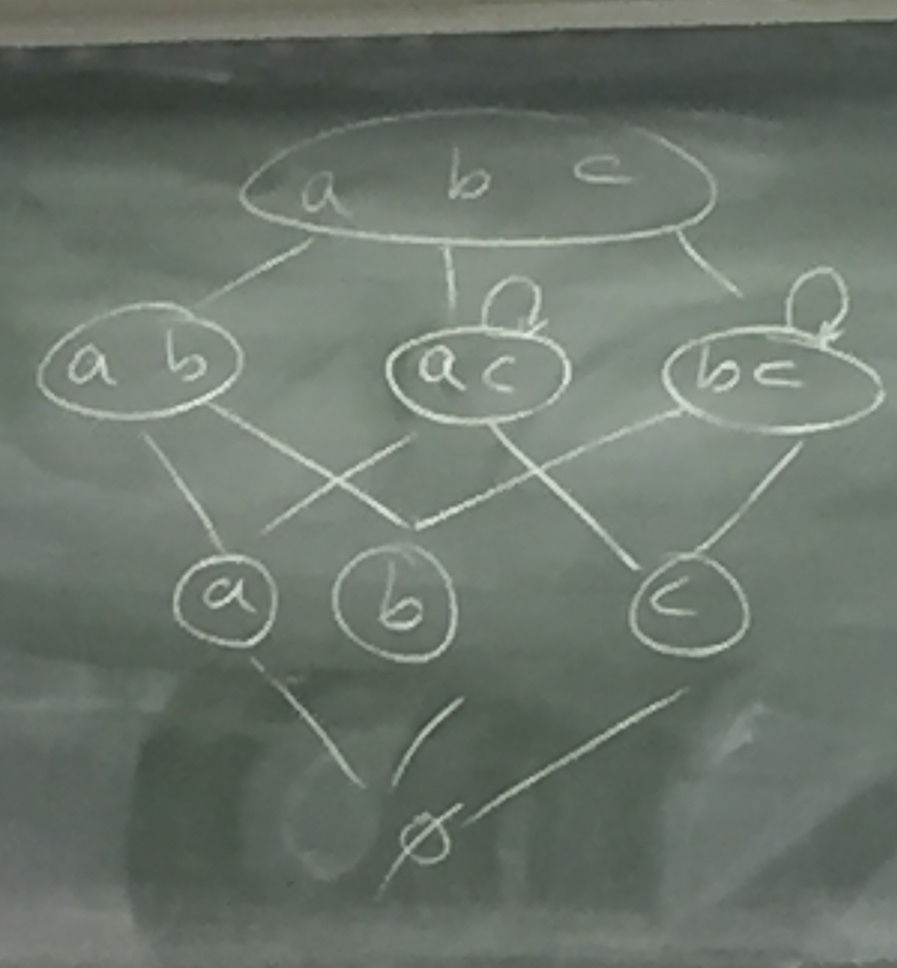
\includegraphics[width=0.7\linewidth]{img/img1}
\caption{}
\label{fig:img1}
\end{figure}
\begin{equation}
\begin{split}
&c \in ac \\
&\tau(c) \subseteq \tau(ac) \\
&\tau(c) = c! \\ % TODO: cancel
&\tau(c) = ac
\end{split}
\end{equation}

\begin{equation}
\begin{split}
&c \in bc \\
&\tau(c) \subseteq \tau(bc) \\
&\tau(c) = c! \\  % TODO: cancel
&\tau(c) = bc
\end{split}
\end{equation}

Dies ist ein Widerspruch


\paragraph{P Datalog-Programm}
$\tau_P$ liefert Fakten von P vereinigt mit Fakten, die in einem Schritt aus der Argumentenmenge von $\tau_P$ mit den Regeln von P abgeleitet werden können.

\subsection*{Ableitung in einem Schritt}

\subsubsection*{Definition: Substitution}
Eine Substitution ist eine endliche Menge der Form
\begin{equation}
\{ X_1 / t_1, \cdots, X_n / t_n \}, X_1,...,X_n \text{ unterschiedliche Variablen, } t_1,....,t_n Terme, X_i \neq t_i
\end{equation}

Falls alle $t_i$ Konstanten sind, ist dies eine \textbf{Grundsubstitution}.

Sei $\theta$ eine Substitution, t ein Term (Variable oder Konstante), so gilt \\

\begin{equation}
t\theta =_{def} \begin{cases} t_i, & \mbox{falls } t/t_i \in \theta \\ t, & \mbox{sonst} \end{cases}
\end{equation}
Sei L ein Literal, $L\theta$ bezeichnet dasjenige Literal, das aus L entsteht, indem alle Variablen $X_i$ mit $L_i$ für die $X_i / t_i \in \theta$ gilt, simultan durch $t_i$ ersetzt werden. Analog $d\theta$ für eine Datalog-Klausel d.

\paragraph{Beispiel}

\begin{equation}
L = p(X, Y, a), \theta = \{X / a, Y / X \} \\
L\theta = p(a, X, a)
\end{equation}

Sei D eine Menge von Datalog Klauseln. In einem Schritt aus D ableitbare Menge von Fakten:

\begin{equation}
fakt_1(D) = \{ f \in HB_D | (\exists Regel L_0 :- L_1,...,L_n)(\exists Sicht \theta)(\{ L_1 \theta, \cdots, L_n\theta \} \subseteq D \wedge f = L_0\theta) \}
\end{equation}

(Annahme: built-in Prädikate geeignet berücksichtigt $\Rightarrow$ Algorithmus FAKT\_1)

Definiere $\tau_P | 2^{HB} \Rightarrow 2^{HB}$. $\tau_P(I) =_{def} P_F \cup fakt_1(P_R \cup I)$.$ P_f = $ Menge der Fakten von P. $P_P$ Menge von Regeln von P.

\subsection*{Satz 1.3} Für jedes Datalog-Programm P ist $\tau_P$ eine monotone Transformation auf $(2^{HB}, \subseteq)$.

\subsubsection*{Beweis}
Seien $I_1, I_2 \in HB_P$ mit $I_1 \subseteq I_2$. z.Z.: $\tau_P(I_1) \subseteq \tau_P(I_2)$. \\
Sei $f \in \tau_P(I_1)$. Falls $f \in P_F$, dann gilt auf $f \in \tau_p(I_2)$. $f \in fakt_1(P_R \cup _1)$ da $I_1 \subseteq I_2$, gilt $P_R \cup I_1 \subseteq P_R \cup I_2$ und somit $f \in fakt_1(P_R \cup I_2)$ wg. Monotonie von Fakt\_1 auf ($2^{HB}, \subseteq$).


\paragraph{Beispiel}

\begin{equation}
\begin{split}
P = &p(1) \\
= &p(2). \\
= &r(1). \\
&\\
q(X) :- &s(X), r(X). \\
s(X) :- &p(X).
\end{split}
\end{equation}

$\leadsto^{T_p(\emptyset)}$

\begin{equation}
\begin{split}
&p_1\\
&p_2 \\
&r_1
\end{split}
\end{equation}

$\leadsto^{T_p(\cdots)}$

\begin{equation}
\begin{split}
&p_1\\
&p_2 \\
&r_1\\
&s(1) (\text{fakt\_1}) \\
&s(2) (\text{fakt\_1})
\end{split}
\end{equation}

$\leadsto^{T_p(\cdots)}$

\begin{equation}
\begin{split}
&p_1\\
&p_2 \\
&r_1\\
&s(1) \\
&s(2) \\
&q(1) (\text{fakt\_1})
\end{split}
\end{equation}

\subsection*{Satz 1.4} Für jedes Datalog-Programm P gilt $cons(P) = lf_p(\tau_p)$ (lf = least fixpunkt).

\subsubsection*{Beweis}:
\paragraph{1)} cons(P) ist ein Fixpunkt von $\tau_P$. \\
$\tau_p(cons(P)) = P_F \cup fakt\_1(P_R \cup cons(P))$. cons(P) ist kleinstes Herbrand-Modell von P, d.h. alle Regeln sind gültig unter $cons(P) \Rightarrow fakt\_1(P_R \cup cons(P) = cons(P) \backslash P_F)$. (und kein Fakt kann aus cons(P) entfernt werden, ohne dass die Modelliereigenschaft verloren geht.) $\Rightarrow \tau_P(cons(P)) = P_F \cup cons(P) \backslash P_F = cons(P)$

\paragraph{2)} $cons(P)$ ist minimaler Fixpunkt von $\tau_P$.\\
Annahme: $(\exists I \not\subseteq cons(P))(\tau_P(I) = I)$.\\
cons(P) ist minimales Herbrand-Modell $\Rightarrow$ I ist kein Herbrand-Modell. Da $P_F \subseteq I$ wg. Annahme $\tau_P(I) = I$ folgt midestens eine Regel ist nicht erfüllt, d.h. $(\exists h_0, \cdot,h_n \in P_R)(\exists Substitution \theta)(\{ h_1\theta, \cdots, L_n(\theta)\} \subseteq I \wedge L_1 \theta \cancel{\in} I)$. Aber $L_0 \in fakt_1(P_R \cup I)$ nach Definitio von fakt\_1.
Da auch $L_0 \theta \in P_F$ wegen $P_F \subseteq I, folgt \tau_P(I) \neq I$. Noch Fixpunkttheorem (Kuaster / Tarski) ist minimaler Fixpuknt von $\tau_P$ kleinster Fixpunkt von $\tau_P$. 

\subsection*{Vorgehensweise bei Fixpunktberechnung} bottom-up

\subsubsection*{Bezeichnung: Forward-chaining}Da ``$\Leftarrow$'' die natürliche Richtung für die Anwendung von Regeln ist.
Da Regeln sicher sind ist $L_i \theta$ stets ein Fakt $\theta_i$.
Betrachte Eignung der Methode zur Anfrageauswertung, z.B. ?- vs(c4, y). ``Alle Kurse, die Voraussetzung von Kurs c4 sind''

\paragraph{Ineffizient} Berechnung des $lf_p$ und anschließende Siche zu vs(c4, y) passende Fakten $\Rightarrow$ Vermeide möglichst Berechnung nicht relevanter Fakten (später).

Starte mit Zielklausel, Suche ein Regel die zu einem Atomder Klausel passt. Ersetze das Atom durch angepassten Rumpf der gewählten Regel, neue Anfrage, iterieren.

\subsubsection*{Bezeichnung: Backward-chaining}
\paragraph{Beispiel}
\begin{equation}
\begin{split}
P = &p(1) \\
= &p(2). \\
= &r(1). \\
&\\
q(X) :- &s(X), r(X). \\
s(X) :- &p(X).
\end{split}
\end{equation}

% TODO: img 3 hier


\subsection*{Prozedurale Semantik}
Beweistheoretische Sicht, übertragen auf Datalog Programm P aufgefasst als Theorie 1. Stufe \\
Semantik: $\{f \in HB_P | P \vdash f \}$ \\
Wie können Ableitungen (Beweise) von Fakten systematisch durchgeführt werden?

Regeln: 
\begin{equation}
\begin{split}
(1) vs(X, Y) &:- Kp(X, Y). \\
(2) vs(X, Y) &:- vs(X, Z), kp(Z, Y). \\
P &= \{ Kp (c4, a3), \cdots, kp(c2, a0), (1), (2) \} 
\end{split}
\end{equation}

Zeige $P \vdash vs(c4, a0)$. 
\begin{equation}
\begin{split}
(1) = (\forall X)(\forall Y)&(kp(X, Y) \Rightarrow vs(X, Y)) \\
(2) = (\forall x)(\forall Y)(\forall Z)&(vs(X, Z) \wedge kp(Z , Y) \Rightarrow vs(X, Y))
\end{split}
\end{equation}

\paragraph{Beweis}
\begin{figure}[h!]
\centering
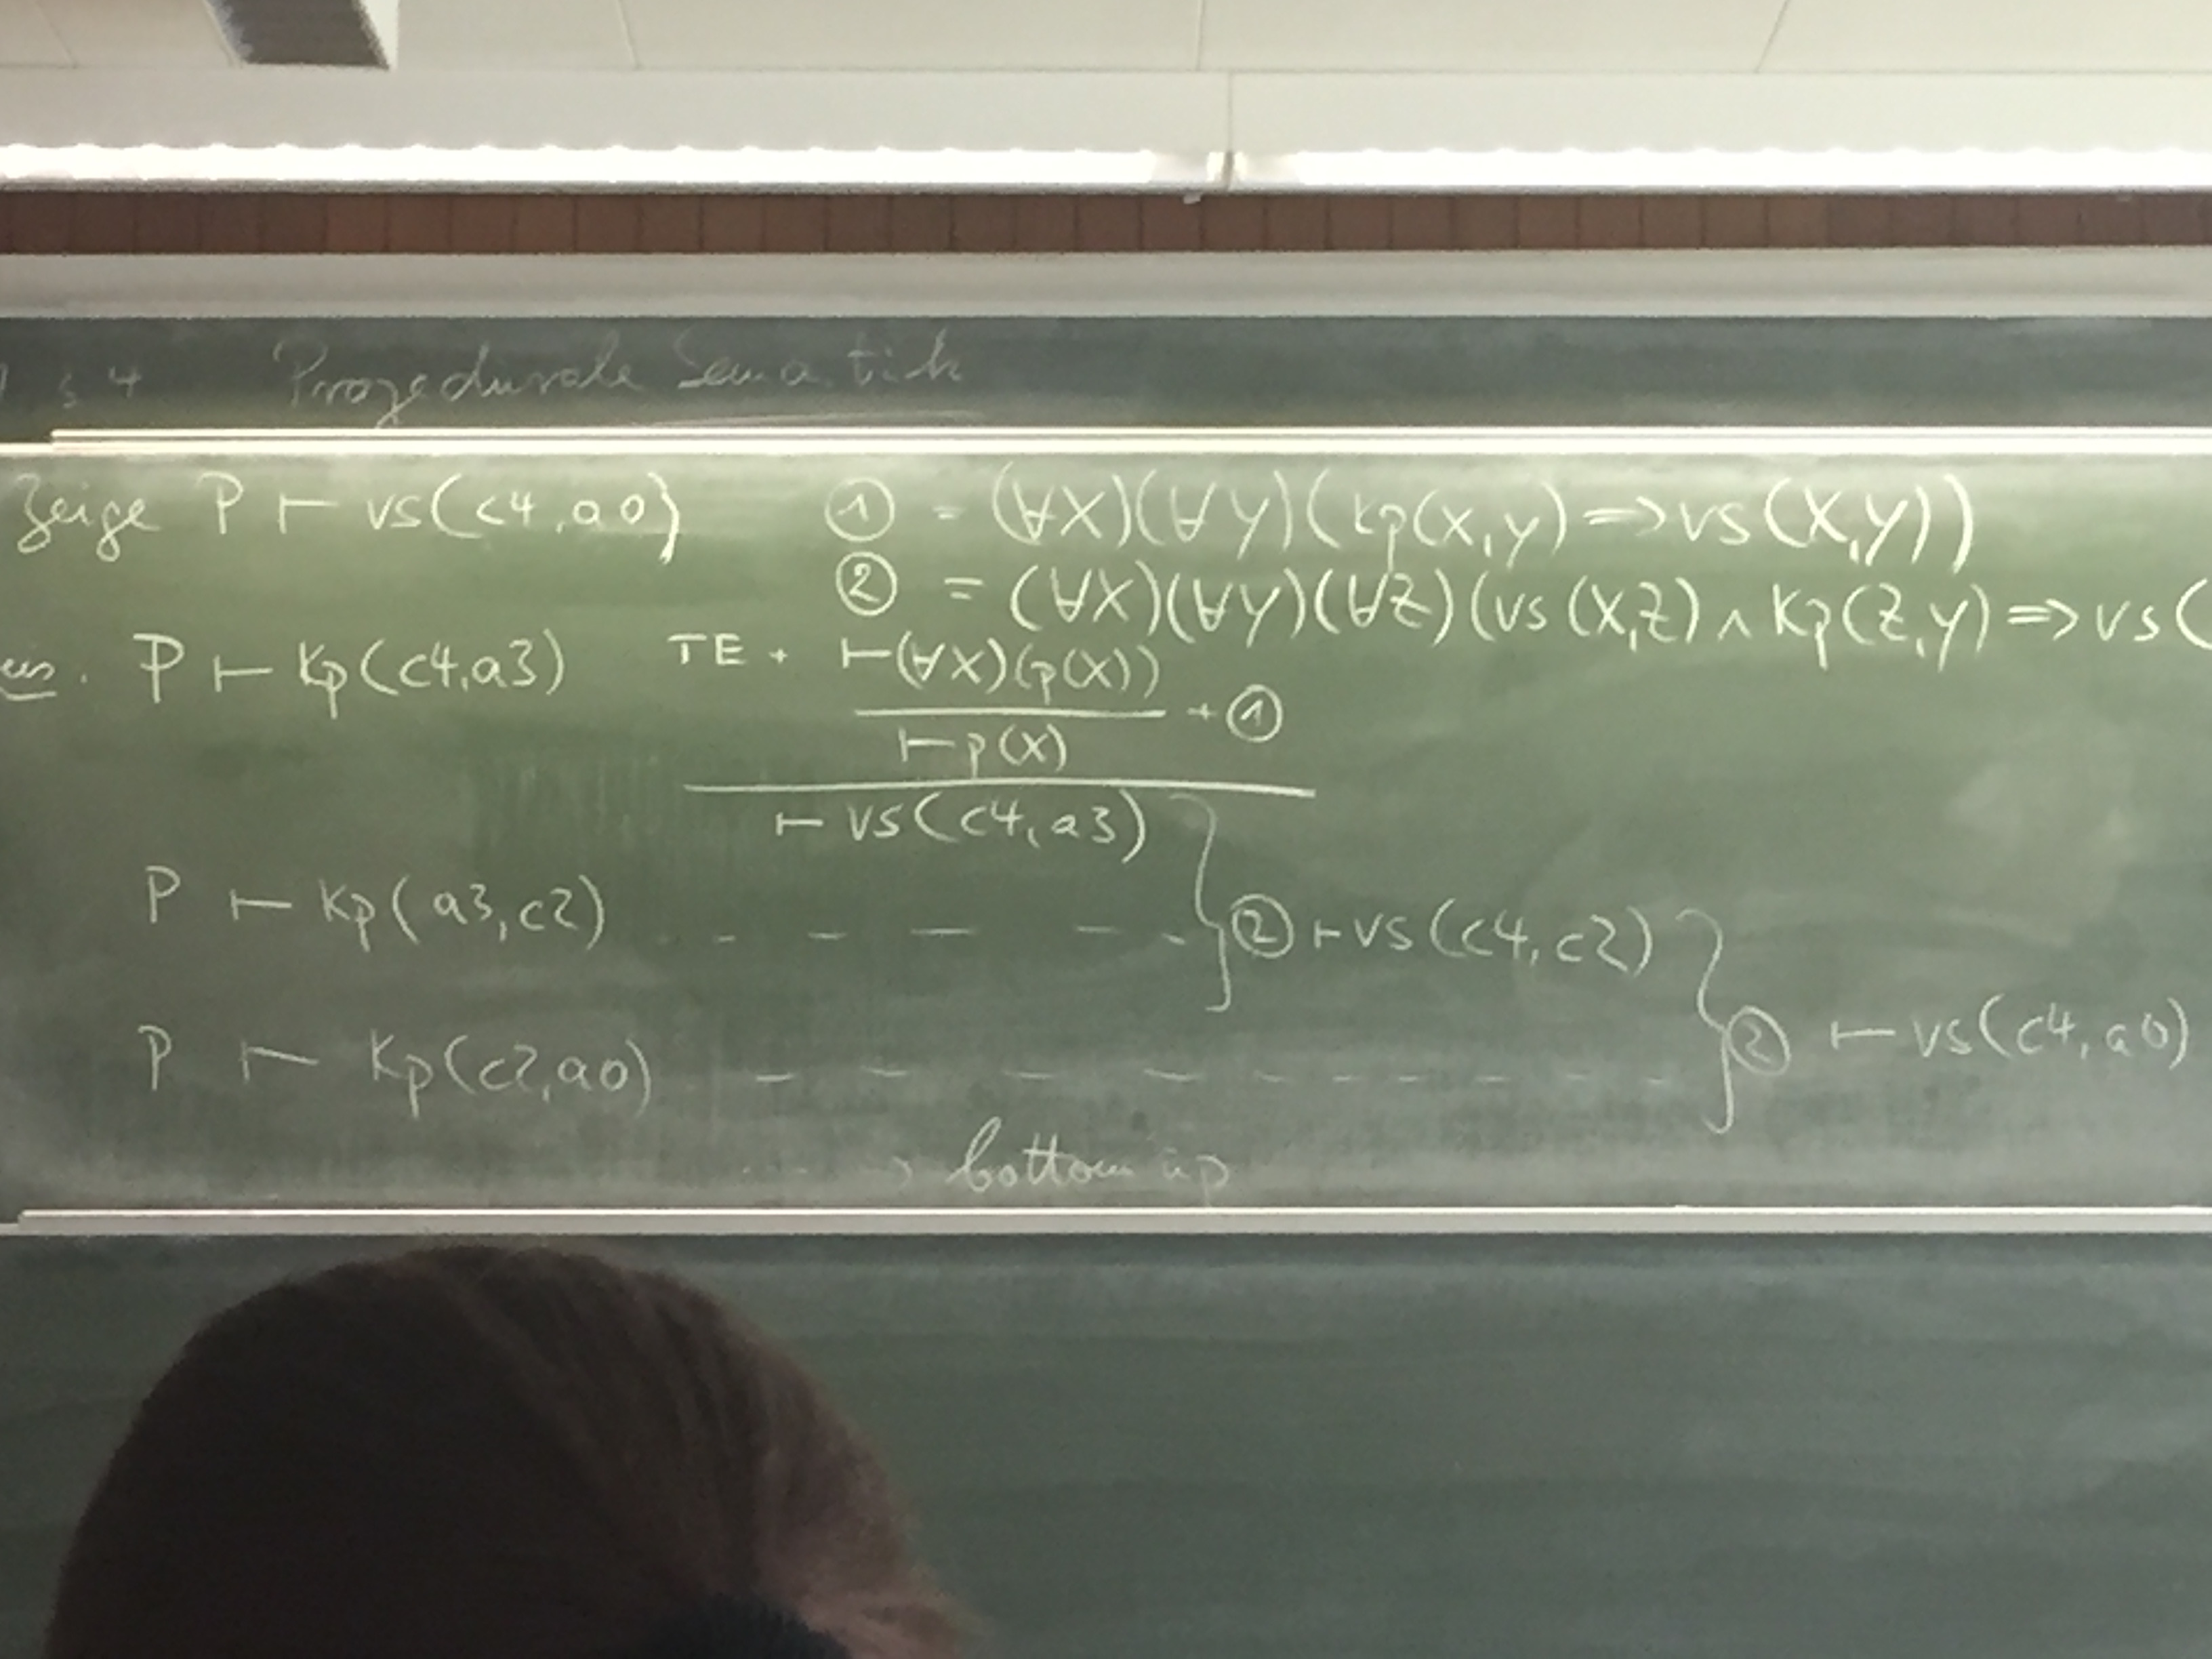
\includegraphics[width=0.7\linewidth]{img/img4}
\caption{}
\label{fig:img4}
\end{figure}
\begin{figure}[h!]
\centering
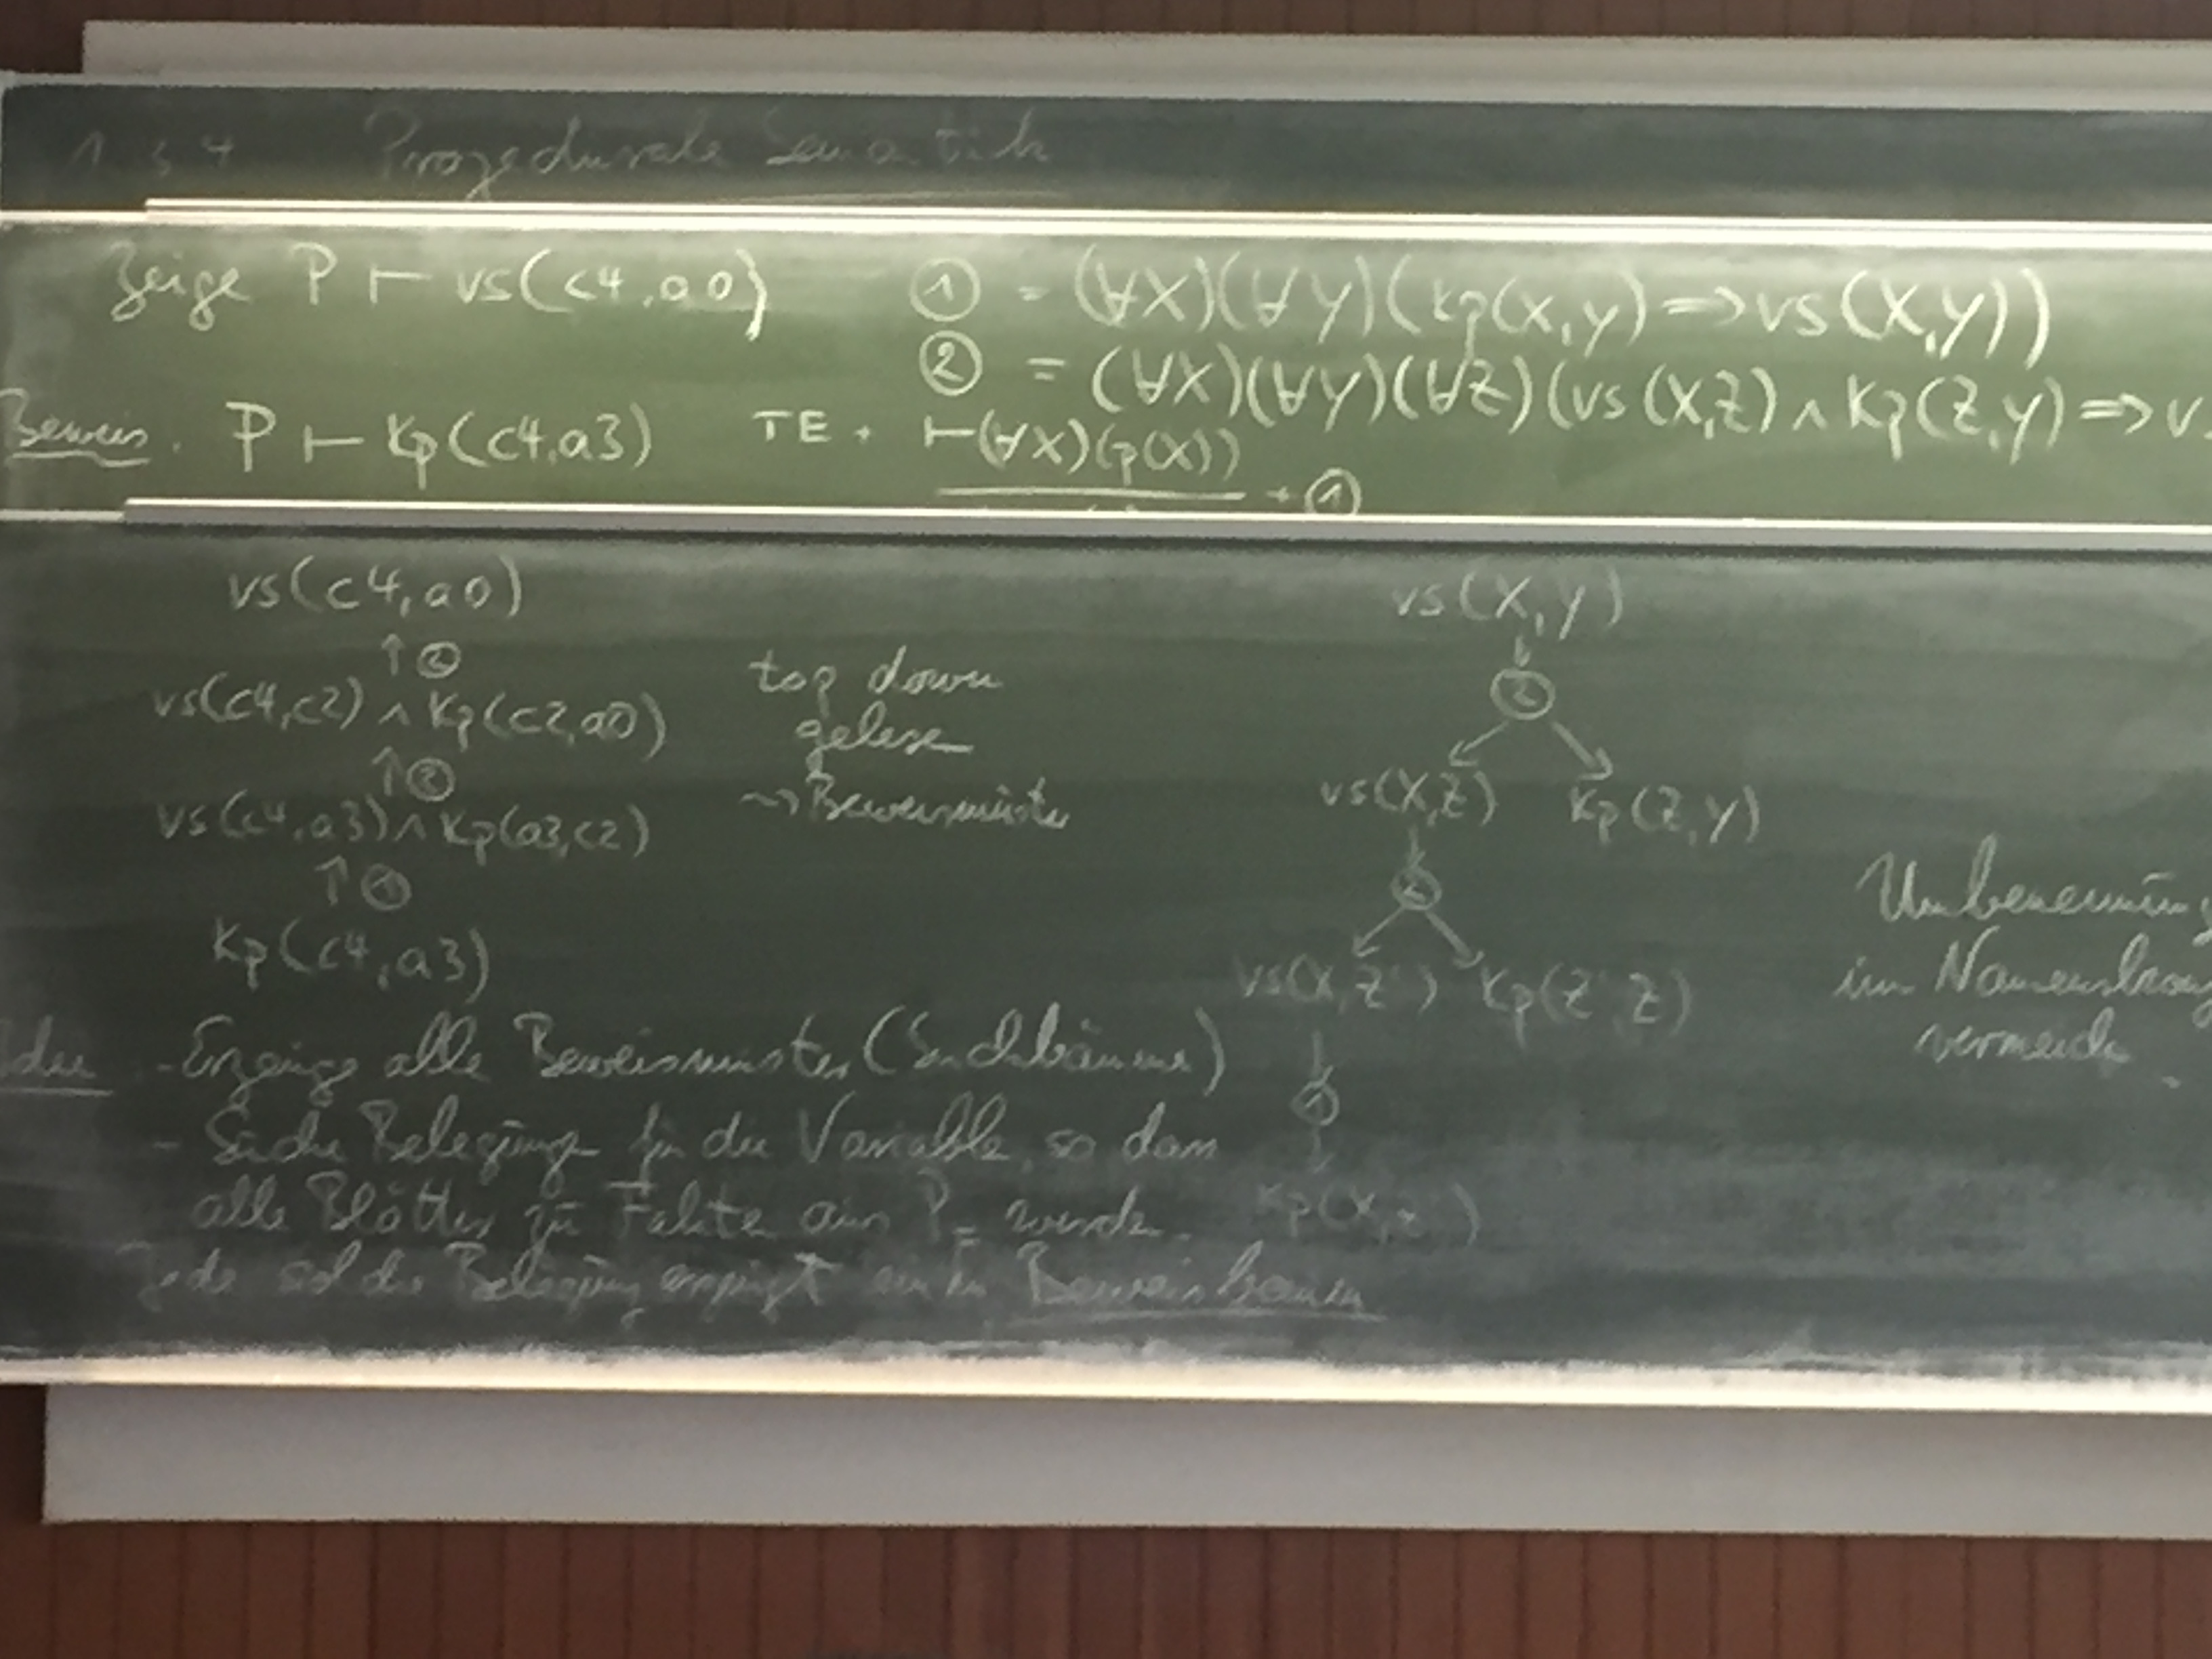
\includegraphics[width=0.7\linewidth]{img/img5}
\caption{}
\label{fig:img5}
\end{figure}

\paragraph{Idee} 

\begin{itemize}
\item Erzeuge alle Beweismuster (Suchbäume)
\item Suche Belegungen für die Variable, so dass alle Blätter zu Fakten aus P werden
\item jede solche Belegung erzeugt einen Beweisbaum.
\end{itemize}

\paragraph{Zunächst} Suche nach ``passenden'' Köpfen von Regeln erfordert Definition.

\subsubsection*{Definition: Unifizierbar}

Seien $L_1$ und $L_2$ heißen \textbf{unifizierbar}, wenn $(\exists \text{ Substitution } \Theta)(L_1\Theta = L_2\Theta)$. $\Theta$ heißt dann \textbf{Unifikator}.

\paragraph{Beispiel}

$L_1 = vs(X, Z)$ \\
$L_2 = cs(X, Y)$ \\
$\Theta = \{ Z / Y \}$ und $\Theta = \{ Y / Z \}$ sind Unifikatoren von dem Paar $L_1, L_2$, aber auch $\Theta = \{ X/a, Y/a, Z/a \}$. Die ersten beiden sind spezifischer als das letzte

$L_1 = q(X, Y ,c) L_2 = q(W, b, Z)$
Unifikation z.B.:
\begin{equation}
\begin{split}
\Theta_1 &= \{ X/W Y/b Z/c \} \\
\Theta_2 &= \{ X/T, W/T, y/b, Z/c \} \\
\Theta_3 &= \{ X/a, W/a, Y/b, Z/c\}
\end{split}
\end{equation}

Nicht unifizierbar:
$L_1 = q(X, c, U) L_2 = q(W, G, Z)$ oder $L_1 = q(X, a, X) L_2 = q(b, Y, Y)$

\subsubsection*{Definition: Komposition}

Sei $\Theta = \{ X_1 / t_1, \cdots, X_n / t_n \}, \varsigma = \{ Y_1 / n_1, \cdots, Y_m / t_m \}$ Substitutionen. \\
Die Komposition $\Theta\varsigma$ von $\Theta$ und $\varsigma$ erhält man aus 
\begin{equation}
X_1 / t_1\varsigma, \cdots, X_m / t_m\varsigma, Y_1 / n_q, \cdots, Y_m / n_m
\end{equation}
Durch Streichen von Elementen der Form Z/Z sowie $Y_i / n_i$ mit $Y_i = X_j$ für ein j$j \in \{1, ..., n\}$

\paragraph{Beispiel} $\theta= \{ X/a,  Y/W \} \varsigma=\{X/ bm Y/ V, W/Z \}$ \\
$\Theta\varsigma = \{ X/a, YZ, W/Z \}$

\subsubsection*{Definition: allgemeinere Substitution}
Seien $\Theta, \varsigma$ Substitutionen, $\Theta$ heißt allgemeiner als $\varsigma \diamondsuit (\exists \text{Substitution} \delta)(\Theta \delta = \varsigma)$.
Seine $L_1, L_2$ Literale. Ein allgemeinster Unifikator (mgu) von $L_1 in L_2$ ist ein Unifikator von $L_1 und L_2$, der allgemeiner als alle anderen Unifikatoren ist.

\paragraph{Beispiel} $\Theta_2$  ist allgemeiner als $\Theta_3$; betrachte $\delta = \{T / a\}$, es gilt $\Theta_2\delta = \Theta_3$. $\Theta_1$ ist allgemeiner als $\Theta_2, \delta = \{ W / T \}$. mgu ist i.A. nicht eindeutig bestimmt. $L_1 = p(X,X) L_2 = p(V,W)$
mgu: \\
\begin{equation}
\begin{split}
&\{ X/W, V/W \} \\
&\{ X / V, W/V\} \\
&\{ V/X, W/X \}
\end{split}
\end{equation}

\paragraph{Beispiel}
$L_1 = q(X,Y,c)\footnote{t1, t2, t3} L_2 = q(W, b, Z) \footnote{k1 k2 k3}$ \\
\begin{figure}[h!]
\centering
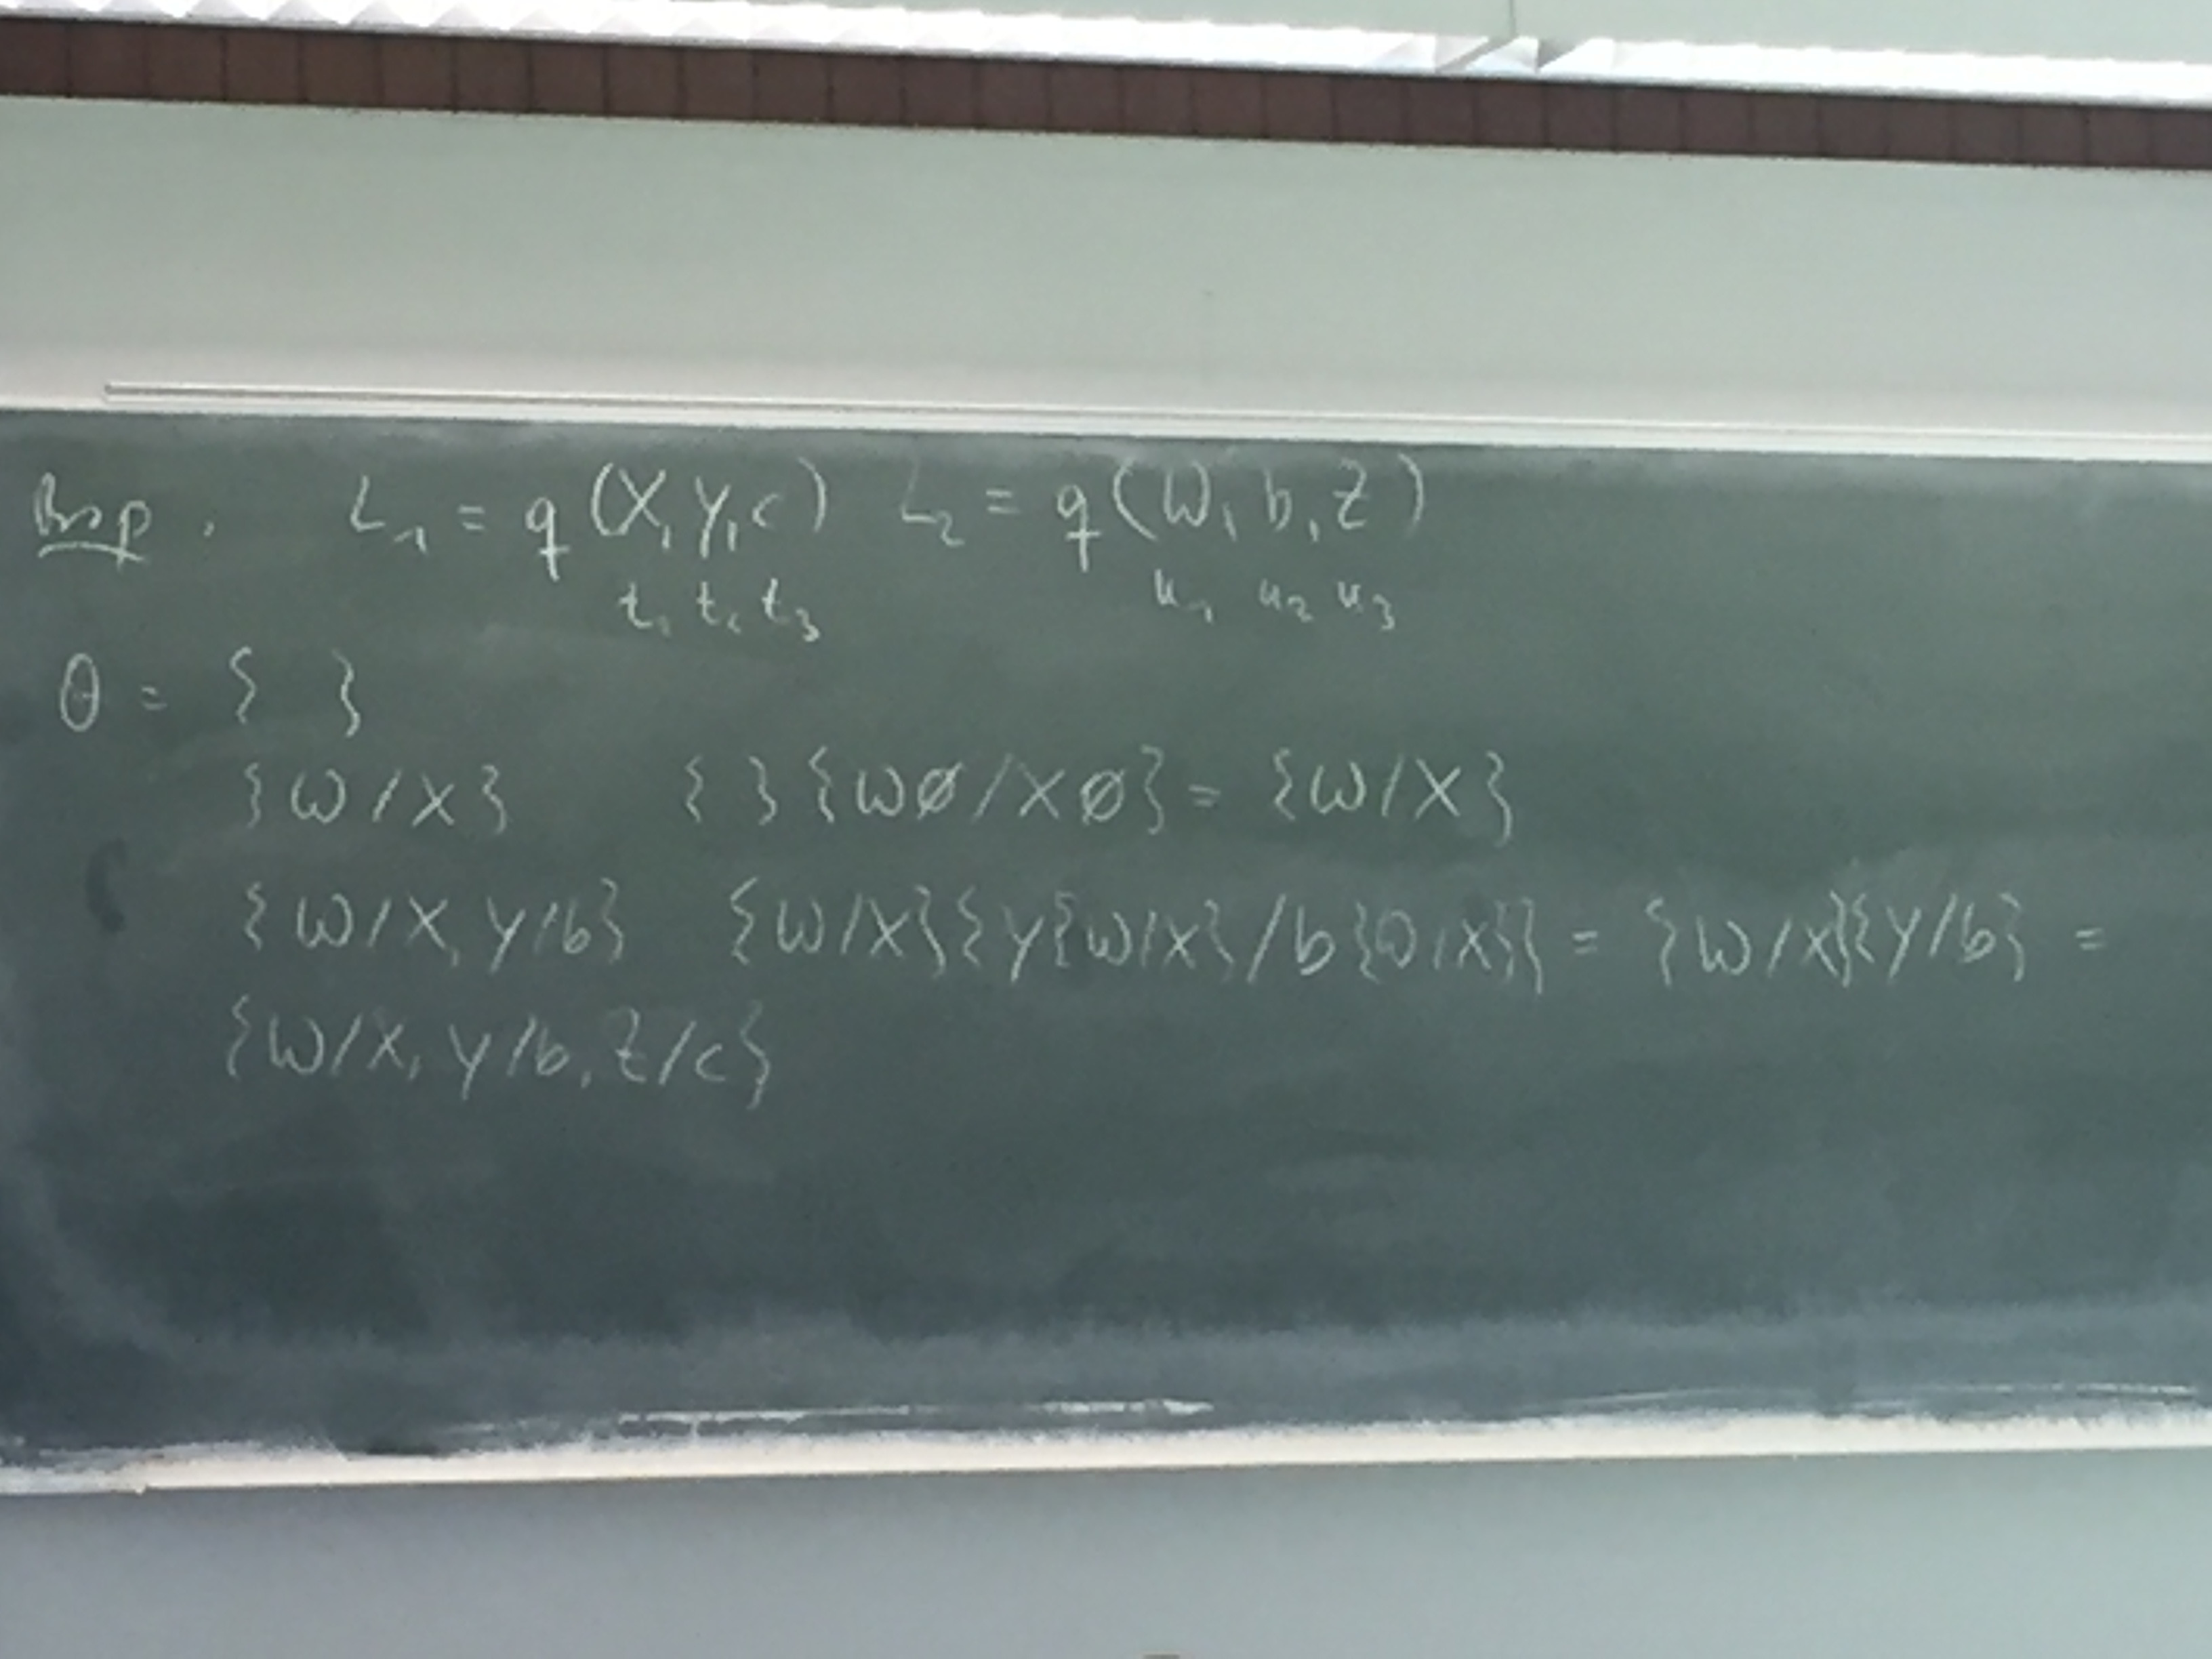
\includegraphics[width=0.7\linewidth]{img/img6}
\caption{}
\label{fig:img6}
\end{figure}


\subsection*{Suchbaum} (Beweismuster zu einem Programm P)
\begin{itemize}
\item Wurzel ist mit einem ``Ziel'' $g = p(t_1, \cdots, t_n), p \in iPr\ddots{a}d$, bekannt.
\item Knoten entlang eines Pfades von der Wurzel aus sind abwechselnd mit Atome und Regeln benannt. (Ziel-, Regelknoten)
\item Alle Blattknoten sind mit Atomen benannt
\item Sei k ein mit einem Atom $a(s_1,...,s_l)$ benannten Knoten (keine Blattknoten), dann ist der unmittelbare Nachfolger von k mit einer Regel von P benannt, deren Kopf mit $q(sq, ..., s_l)$ unifizierbar ist
\item sei k' ein mit einer Regel $r = L_0 :- L_1,...,L_m$ benannte Knoten der unmittelbare Vorgänger von k' sei mit $q(s_1,...,s_l)$ benannt. Dann hat k' m unmittelbare Nachfolger, die mit $I_1 mgu(q(s_1, ..., s_l), I_{0}^{~}), ..., I_m mgu(q(s_1,...,s_l), I_0)$ benannt sind. Dabei sind $I_0, .., I_m$ Atome, die aus $L_1,...,L_m$ durch eventuelle Umbenennung von Variablen hevorgehen (die Variablen seien stets so umbenannt, dass sie im Baum eindeutig sind).
\end{itemize}

\paragraph{Beispiel}
\begin{figure}[h!]
\centering
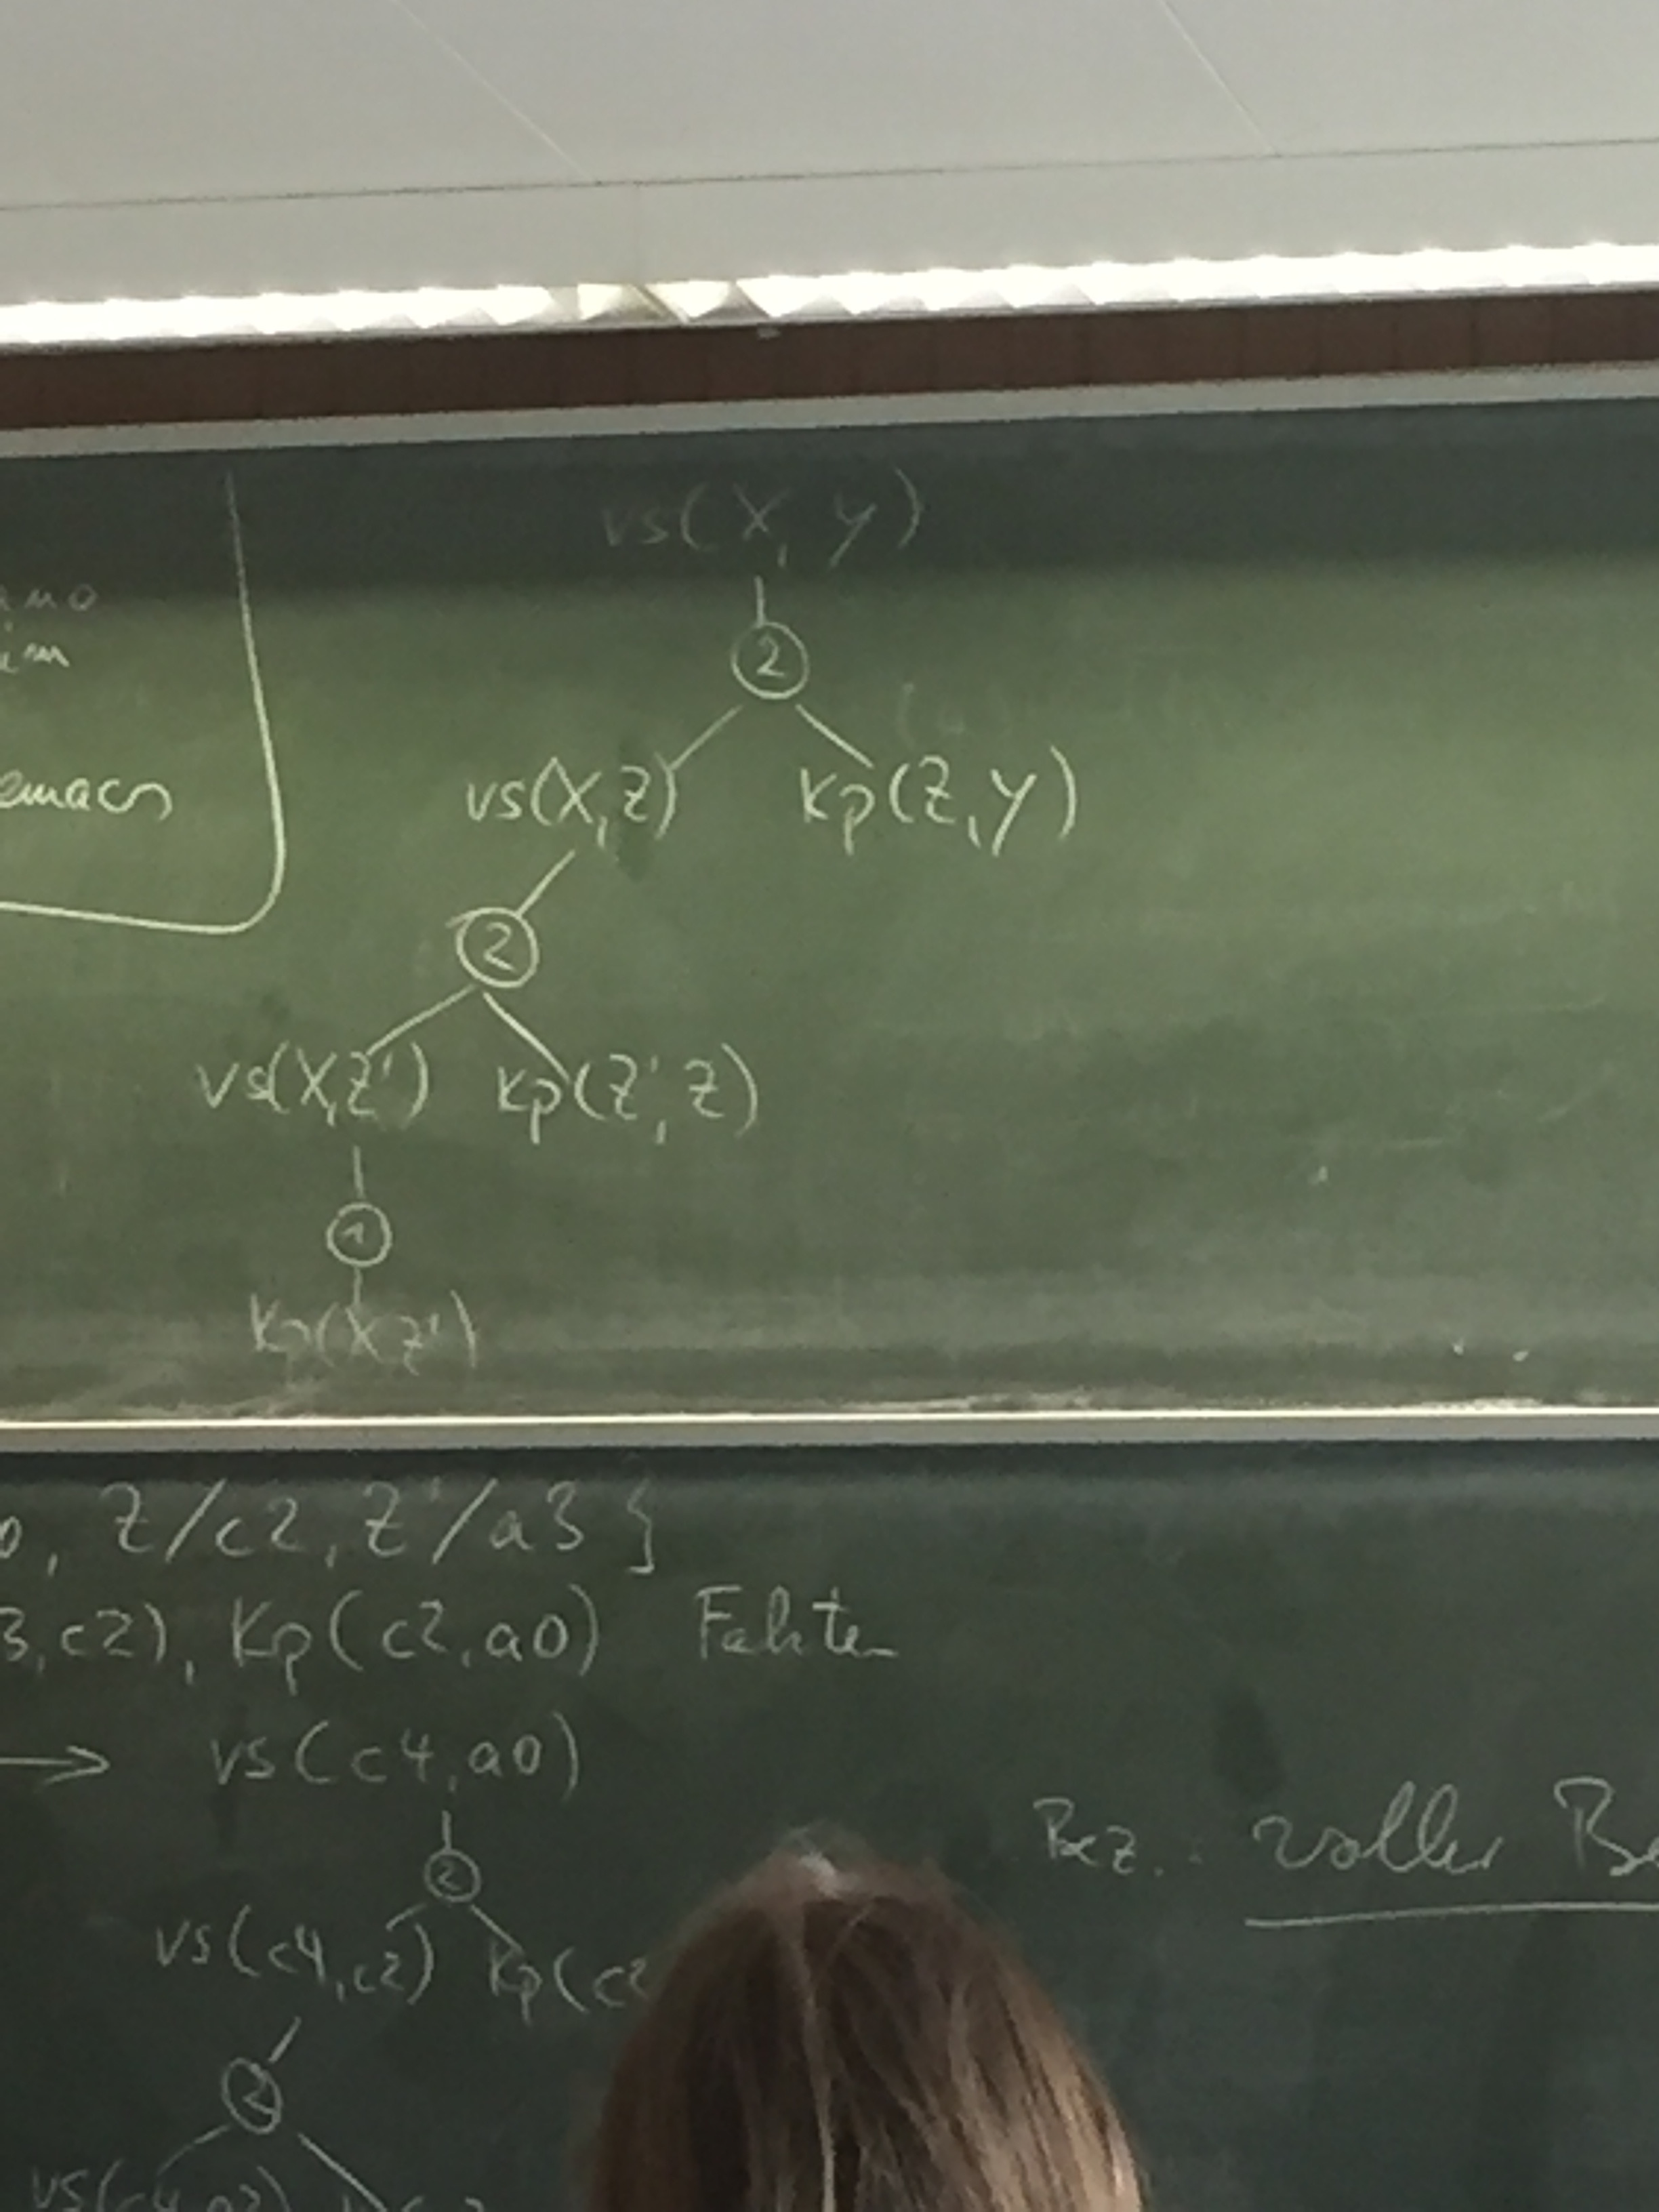
\includegraphics[width=0.7\linewidth]{img/img7}
\caption{}
\label{fig:img7}
\end{figure}

\subsubsection*{Suchbaum $\rightarrow$ Beweisbaum}
Gegeben Sei der Suchbaum S und eine Grundsubstitution $\Theta$ mit folgenden Eigenschaften:
\begin{itemize}
\item $\Theta$ ordnet jeder Variable in S ein Konstantensymbol aus der Menge der in P vorkommenden Konstantensymbole zu.
\item Für jedes Blatt von $S$ gilt, dass $\Theta$, angewand auf die Benennung des Blattes, einen Fakt aus $P_F$ liefert (build-in-Prädikate seien entsprechend berücksichtigt)
\end{itemize}

\paragraph{Beweisbaum} B entsteht aus S durch Anwendung von $\Theta$ auf alle Benennungen von Zielknoten. B repräsentiert einen Beweis für $g\Theta$, g benennung der Wurzel von S.

\paragraph{Beispiel:}
\begin{align*}
\Theta &= \{ X / c4, Y / a0, Z c2, Z'/ a3 \} \\
&kp(c4,a3), kp(a3, c2), kp(c2, a0)  \text{ Fakten}\\
\end{align*}

\begin{figure}[h!]
\centering
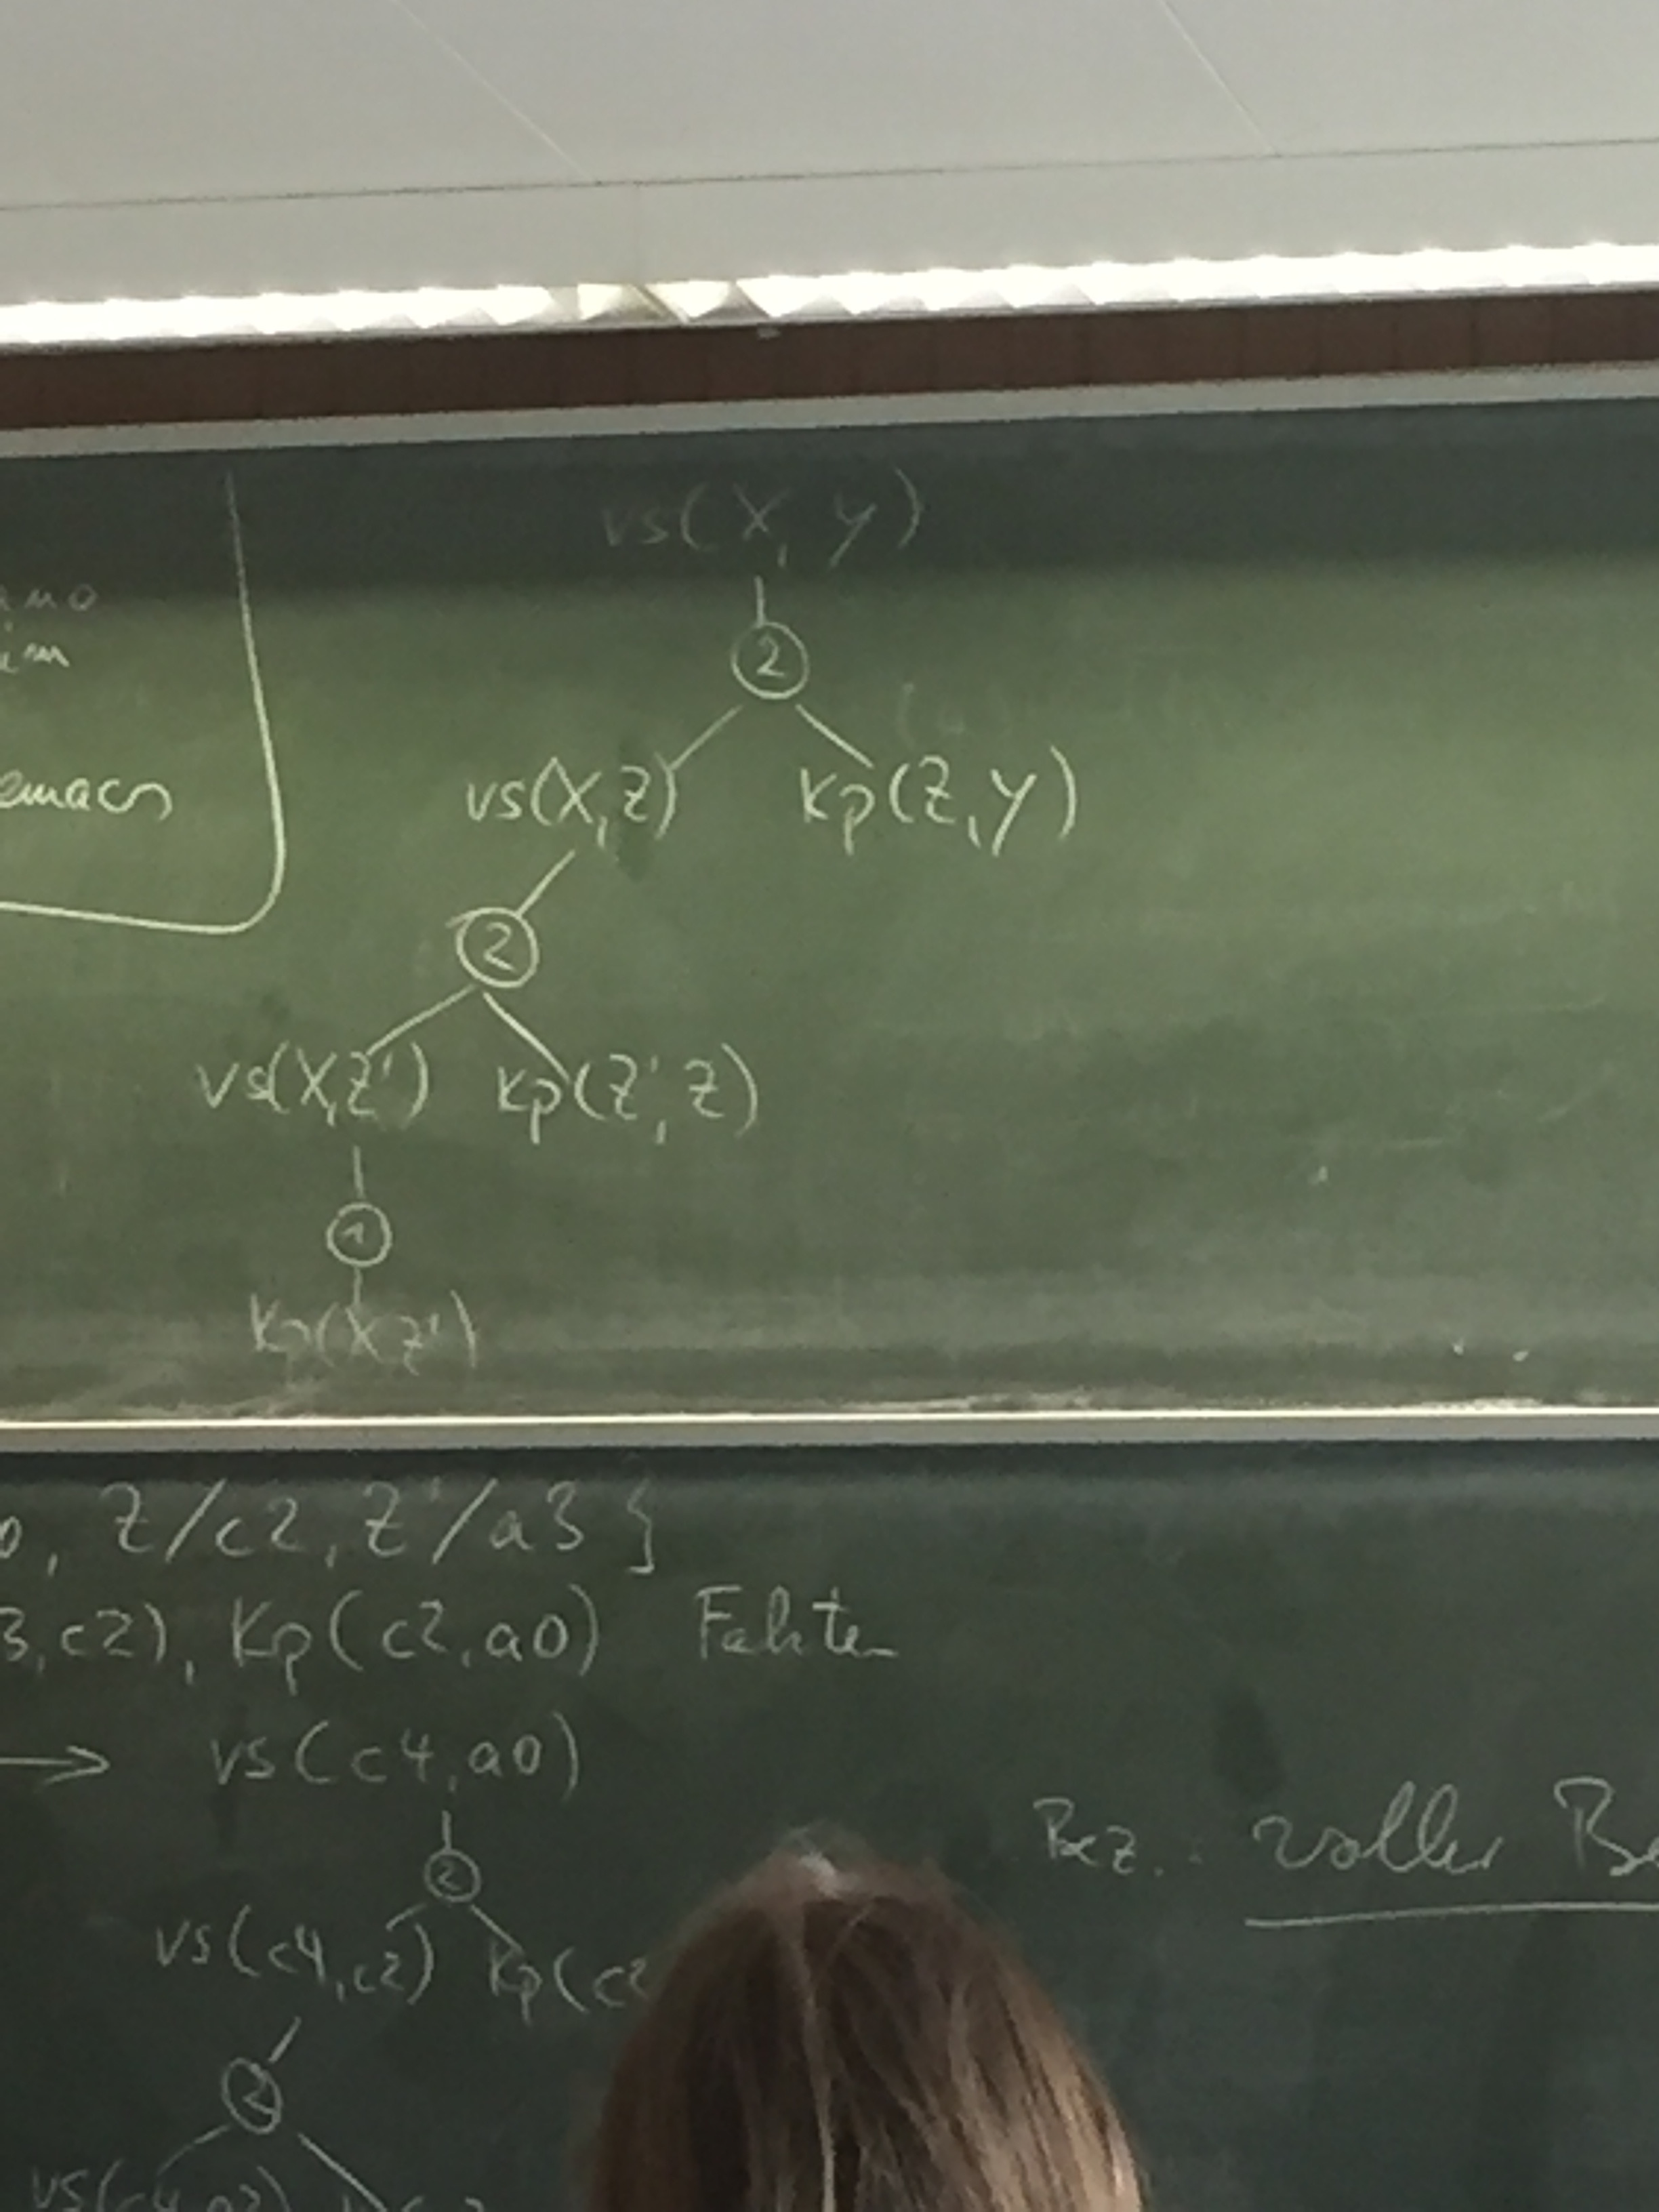
\includegraphics[width=0.7\linewidth]{img/img7}
\caption{}
\label{fig:img7}
\end{figure}

\paragraph{Bezeichnung}: Voller Beweisbaum

\subsubsection*{Systematische Erzeugung der Suchbäume}
Sukzessive alle Bäume der Tiefe 1,2, ... Erzeugen (breadth first)

\paragraph{Definition: Tiefe eines Baums} maximale Anzahl von Zielknoten auf einem Pfad von einem Blattknoten zur Wurzel. Entsprechend Knoten der Tiefe i, Ebene i eines Baumes. Zusätzlich: Spezielle Suchbäume (Tiefe 0) für Fakten aus P.

\paragraph{Beispiel}: Ziel $g = vs(c4, y)$ \\

\begin{itemize}
\item \textbf{Tiefe 1}: vs(c4, y), $\Theta$, kein Beweisbaum
\item \textbf{Tiefe 2}: vs(c4, y)  \\
kp(c4,y), $\{ y / a3 \}$
\end{itemize}

% TODO: Insert Image 8

\paragraph{Offensichtlich}
\begin{itemize}
\item Zu jedem endlichen Beweise, der mit Grundatomen ``Startet'', kann ein entsprechender Beweisbaum auf den beschriebenen Weg erhalten werden.
\item Zu jedem Fakt  $f \in cons(P)$ gibt es einen endlichen Beweis, der mit Grundatomen startet, siehe Fixpunktberechnung $\rightarrow$ voller Beweisbaum
\end{itemize}

$\Rightarrow$ Methode Suchbaum / Beweisbaum ist vollständig. \\
Da ein Beweisbaum mit $g\Theta$ als Benennung der Wurzel einen Beweis für $g\Theta$ darstellt $\Rightarrow$ Methode Suchbaum / Beweisbaum ist korrekt.


\subsection*{Satz 1.5} Sei P ein Datalog-Programm. Die Suchbaum  / Beweisbaum Methode, angewand auf alle Ziele $q(X_1, \cdots, X_{Stelligkeit(q)})$, q intentionales Prädikatesymbol von P, liefert cons(P) als Ergebnis

\paragraph{Frage:} Abbruchkriterium bei der Erzeugung von Suchbäumen

Es gilt
\begin{itemize}
\item Beweisbäume sind isomorph zu den Suchbäumen, aus denen sie erzeugt wurden
\item Zu jedem Fakt $f \in cons(P)$ gibt es einen vollen Beweisbaum, in dem auf jeder Zielknotenebene ein neuer Fakt (neues Teilziel) auftritt
\paragraph{Beweis}
Sei B ein voller Beweisbaum, der diese Eigenschaft nicht erfüllt.
Dann gibt es ein i, so dass in B auf Ebene i nur Fakten auftreten, die schon auf vorhergehenden Ebenen auftreten. Die Teilbäume von B mit Wurzel auf Ebene i können ``höher gehängt'' werden $\Rightarrow$ Es gibt einen äquivalenten, vollen Beweisbaum mit geringerer Tiefe.

\item Es gibt nur endlich viele verschiedene Grundatome, die aus den Prädikaten und Konstantensymbolen gebildet werden können. Konkret: Seien ap(p) die Anzahl verschiedener Prädikatensymbole die in p vorkommen
\item ak(p) die Anzahl verschiedener Konstantensymbole, die in P vorkommen
\end{itemize}

Dann ist $max. fakt(P) = ap(P) * ak(P)^{max\_st(P)}$ eine obere Schranke für die Anzahl verschiedener Grundatome. \textbf{Damit:}
    
\subsubsection*{Satz 1.6} Die Suchbaum / Beweisbaum Methode bleibt vollständig für ein Programm P, wenn nur Bäume mit max. Tiefe max\_fakt(P) betrachtet werden.
Statt breadth first andere Vorgehensweise denkbar:

\begin{itemize}
    \item Depth first mir Abbruch bei max\_fakt(P) und backtracking
    \item Dynamische Abbruchbedingungen, abhängig von erzeugten Faktenmenge (limit 10)
    \item Erkennen und Ausnutzen identischer (Teil-) Zielknoten ($\leadsto$ gerichteter, azyklischer Graph)
\end{itemize}

Zusammenfassen von Such und Beweisbäumen, Berücksichtigung von Fakten aus $P_F$ $\Rightarrow$ frühzeitiges Erkennen von Suchbäumen zu denen keine Beweisbäume existieren

\begin{figure}[h!]
\centering
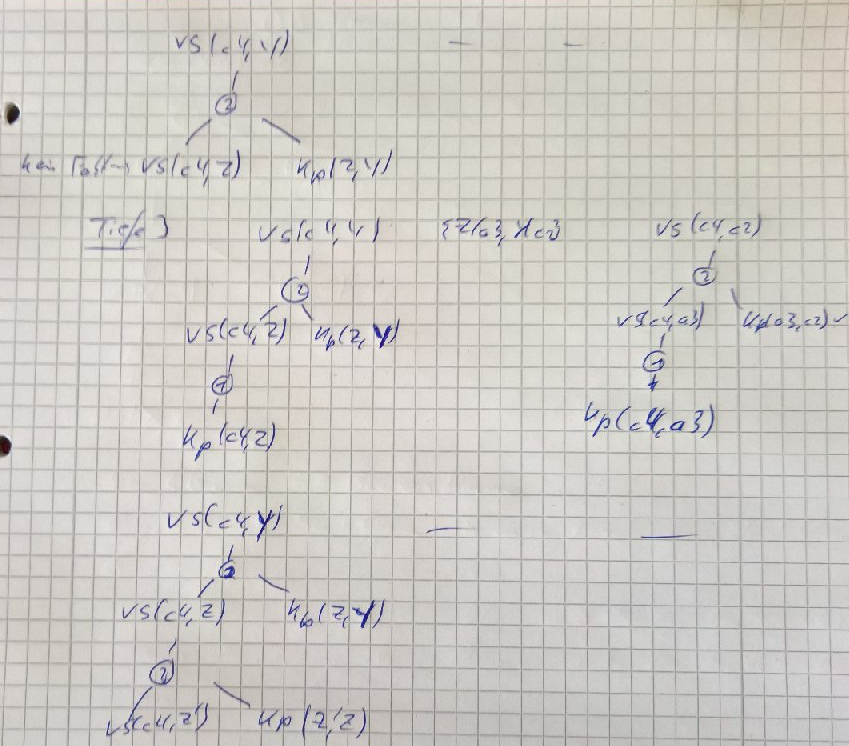
\includegraphics[width=0.7\linewidth]{img/img8}
\caption{}
\label{fig:img8}
\end{figure}

Sei g das Ziel (Wurzelbenenung), dann erzeugt ein Baum der mit der leeren Menge endet, genau ein Ergebnis. 
\begin{align*}
&g \Theta_1, ..., \Theta_n, (\Theta_1, ...., \Theta_n \text{die in dieser Reihenfolge angewandten Unifikatoren (von der Wurzel aus)} \\
&\Theta = \Theta_1, ..., \theta_n \text{ heißt Antwortsubstitution.}
\end{align*}

\subsection*{Resolutionsmethode}

Für allgemeine Klauselformen entwickelte Methode zum automatischen Beweisen.
\paragraph{Literatur} J Allen Robinson: A machine-oriented logic base on the resolution principle. Journal of the ACM 12, S.23-41, 1965 \\

In Logikprogrammierung (Horn-Klauseln): SLD-Resolution (Linear Resolution with Selected Function for Definite Clauses).

\begin{itemize}
\item S (Selection function): Legt fest, wie Literale aus einem Ziel (Klausel mit einem oder mehreren negierten Literalen) auszuwählen sind
\item L (Linear): In jedem Schritt wird genau ein Literal ausgewählt für die Unifikation mit dem Kopf einer Regel einer einem Fakt
\item D (Definit): Beschränkung auf Programme mit definiten Klauseln
\end{itemize}

\paragraph{Bemerkung} Methode steht für ganze Klasse von Algortihmen. Methode auch bekannt unter LUSH (Linear resolution with Unrestricted Selection function for Horn clauses) \\
\paragraph{Übergang Such / Beweisbaum $\leadsto$ Resolution}
Nachweis der Unerfüllbarkeit einer Klausel

\begin{figure}[h!]
\centering
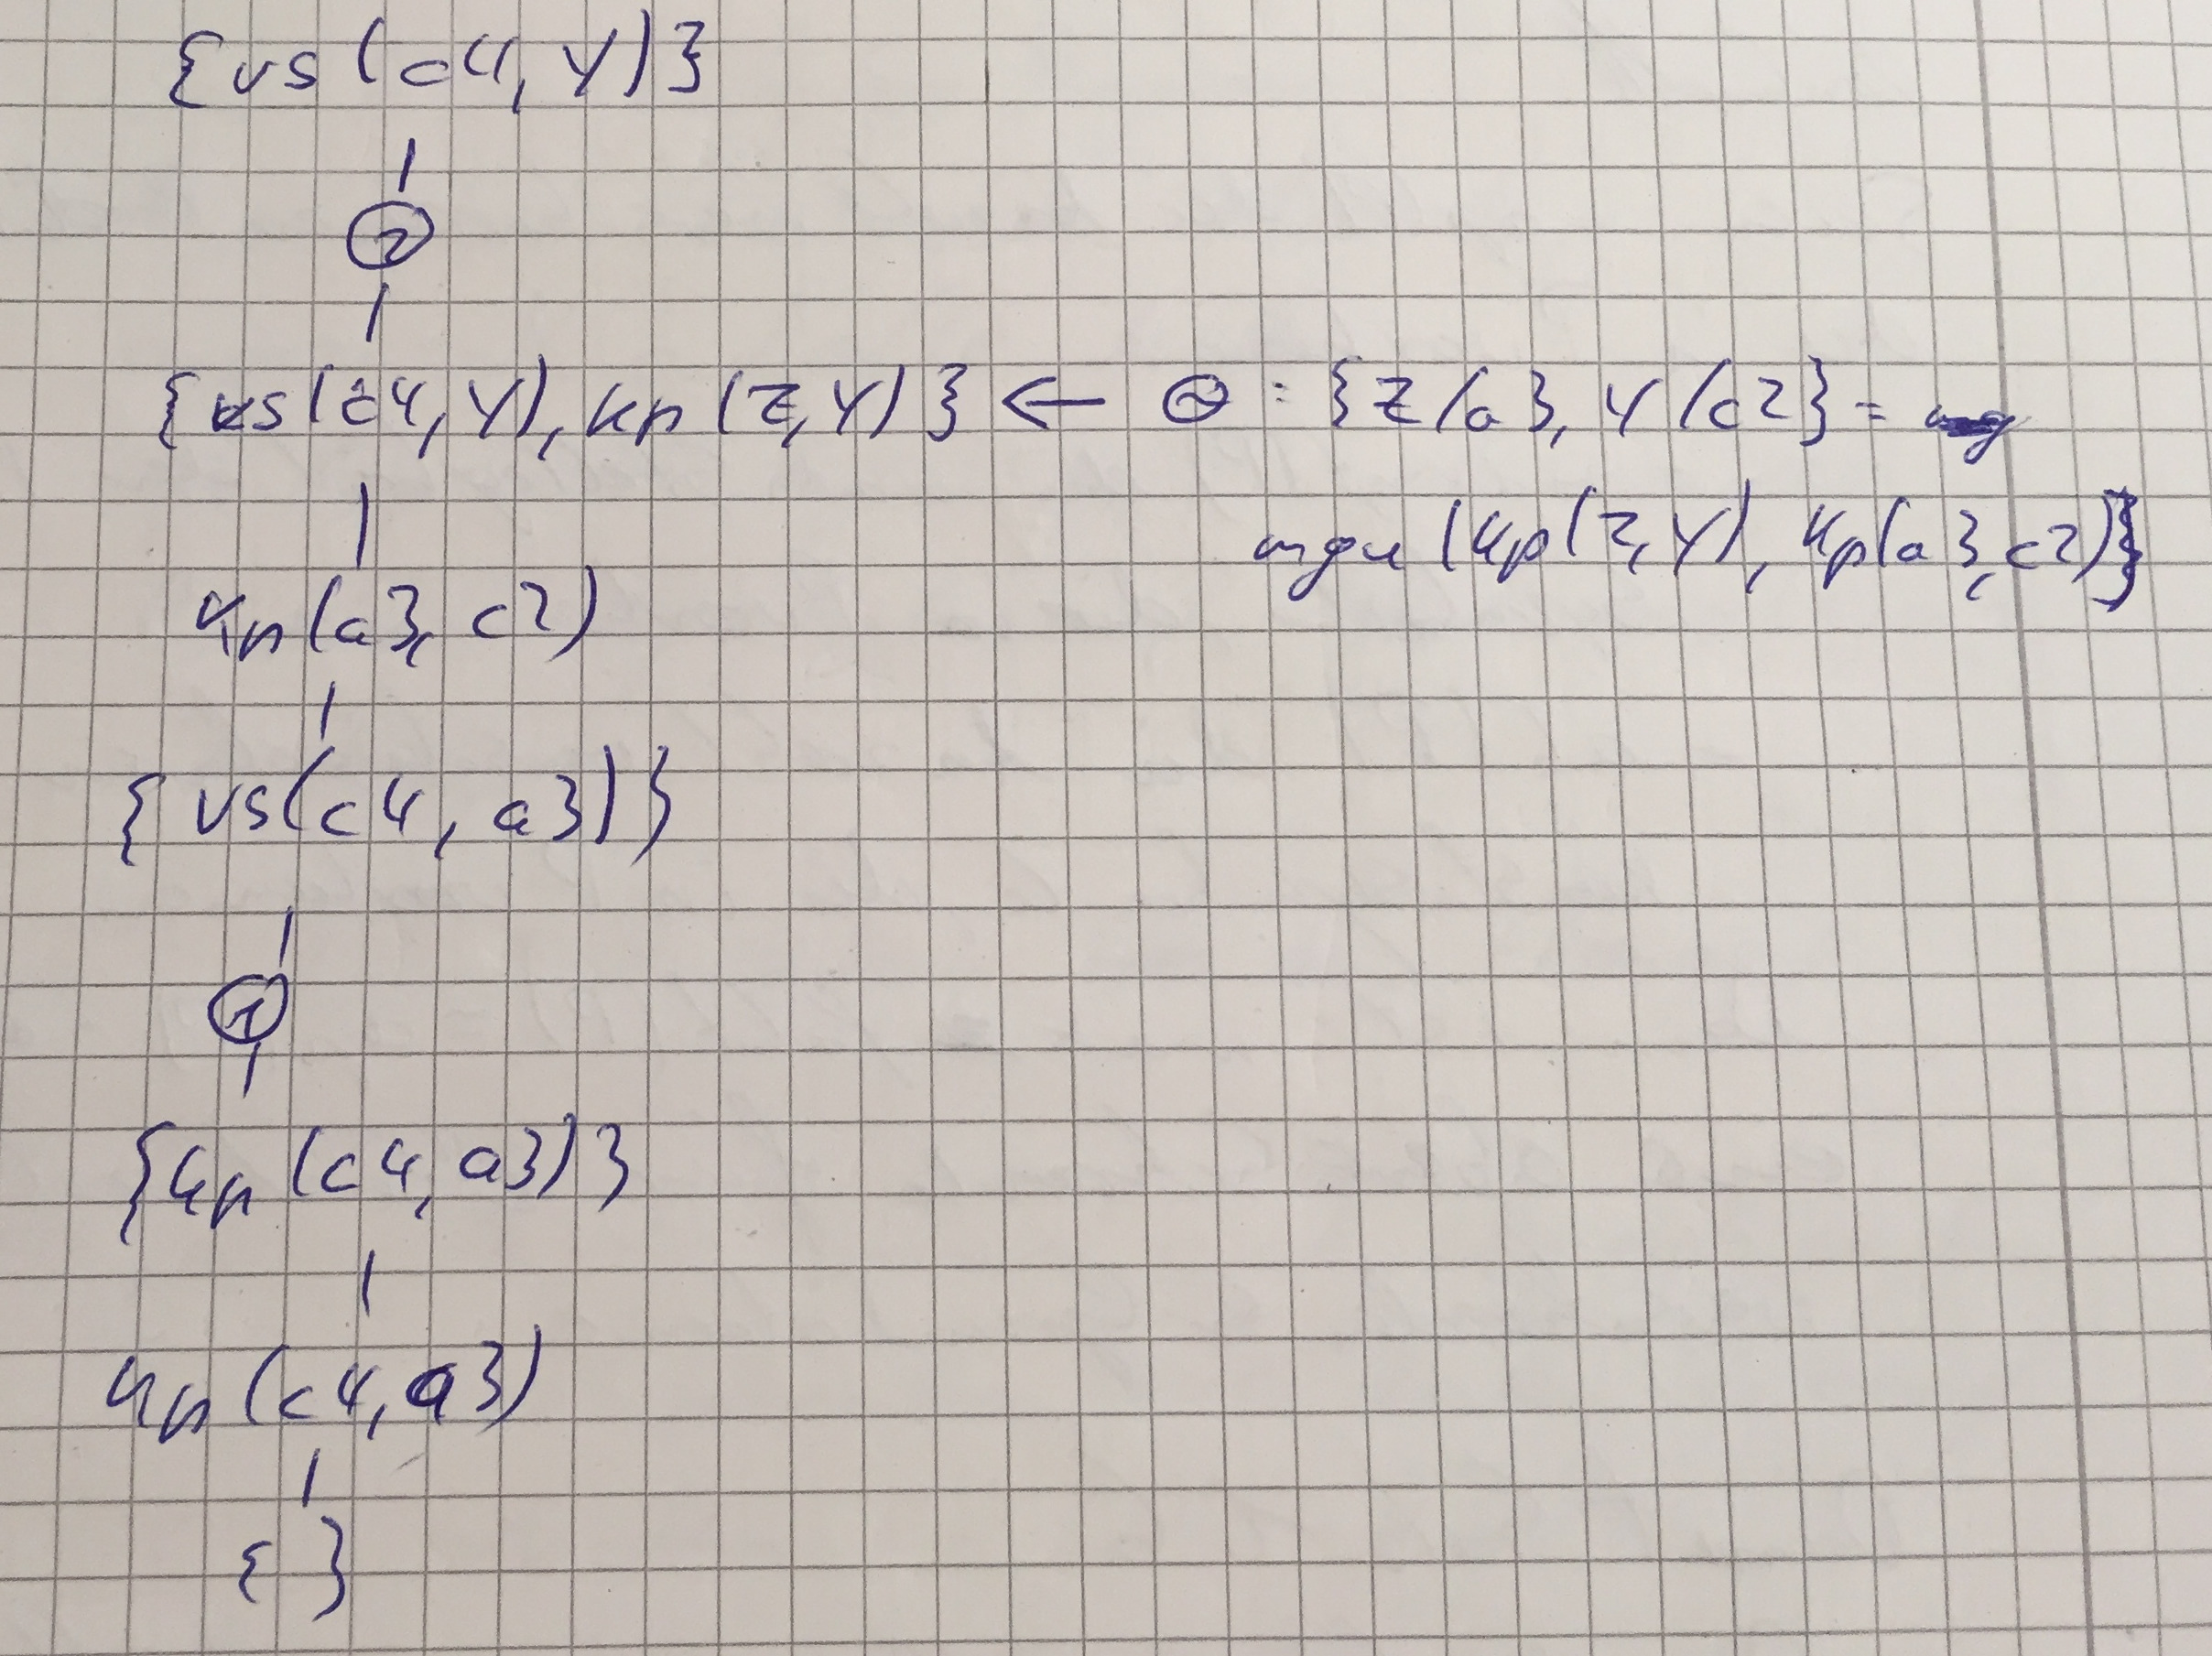
\includegraphics[width=0.7\linewidth]{img/img9}
\caption{}
\label{fig:img9}
\end{figure}


Seien $E = \{ \lnot M_1, \cdots, \lnot M_i, \cdots, \lnot M_K \}, r = L_0 :- L_1, \cdots, L_m$ eine Regel und $S(E) = \lnot M_i$. Es existiere $mgu(M_i, L_0) = 0$.
\paragraph{Resolvente von E und r:} $\{ \lnot M_1\Theta, \cdots, \lnot M_{i-1}\Theta, \lnot L_1 \Theta, \cdots, \L_m \Theta \lnot M_{i + 1} \Theta, \cdots, \lnot M_K\Theta \}$
\begin{itemize}
\item Unerfüllbarkeit: Anwendung der Methode ende mit $\square$ (leere Klausel, entspricht Falsch)
\item Ergebnis: Sei $g = \{ \lnot p(t_1, \cdots, t_n) \}$ das Ziel, $\{ p(t_1, \cdots, t_n)\Theta / \Theta$ Antwortsubstitution für eine Ableitung von g, die mit $\square$ endet \}



Ohne Beweis.

\subsection*{Satz 1.7}
Die SLD-Resolution liefert korrekte und vollständige Ergebnisse für alle Datalog-Programme.

\begin{figure}[h!]
\centering
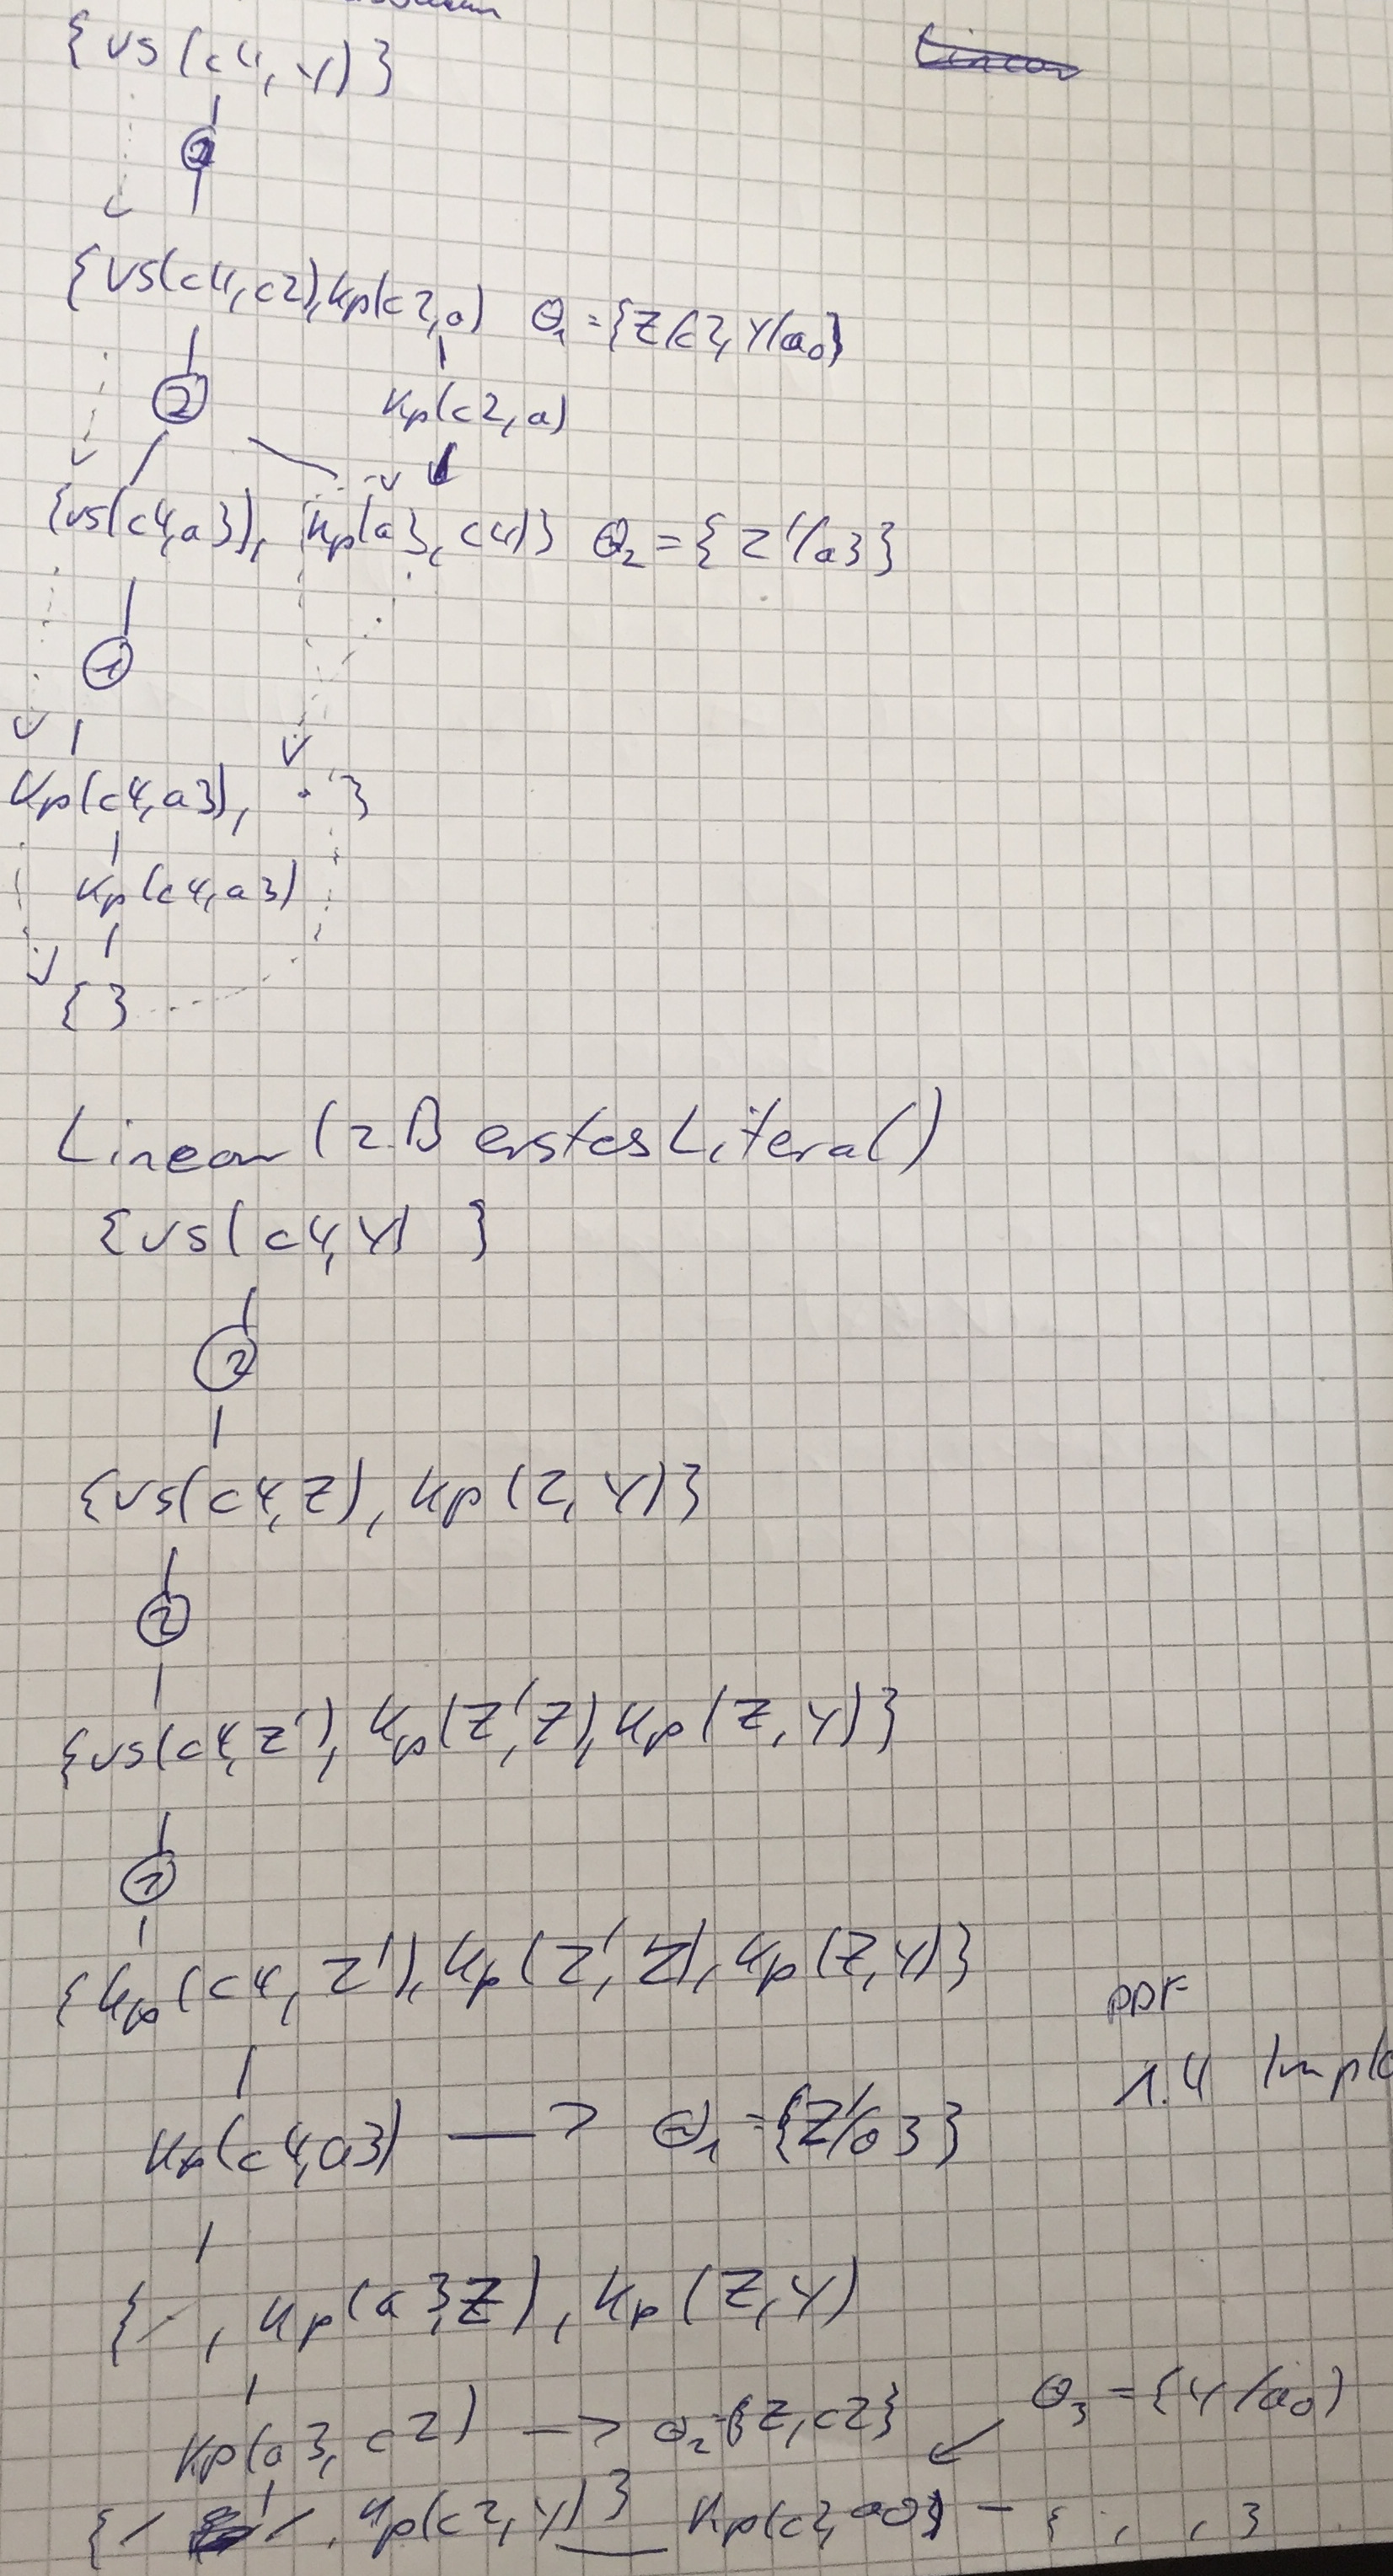
\includegraphics[width=0.7\linewidth]{img/img10}
\caption{}
\label{fig:img10}
\end{figure}
\begin{figure}[h!]
\centering
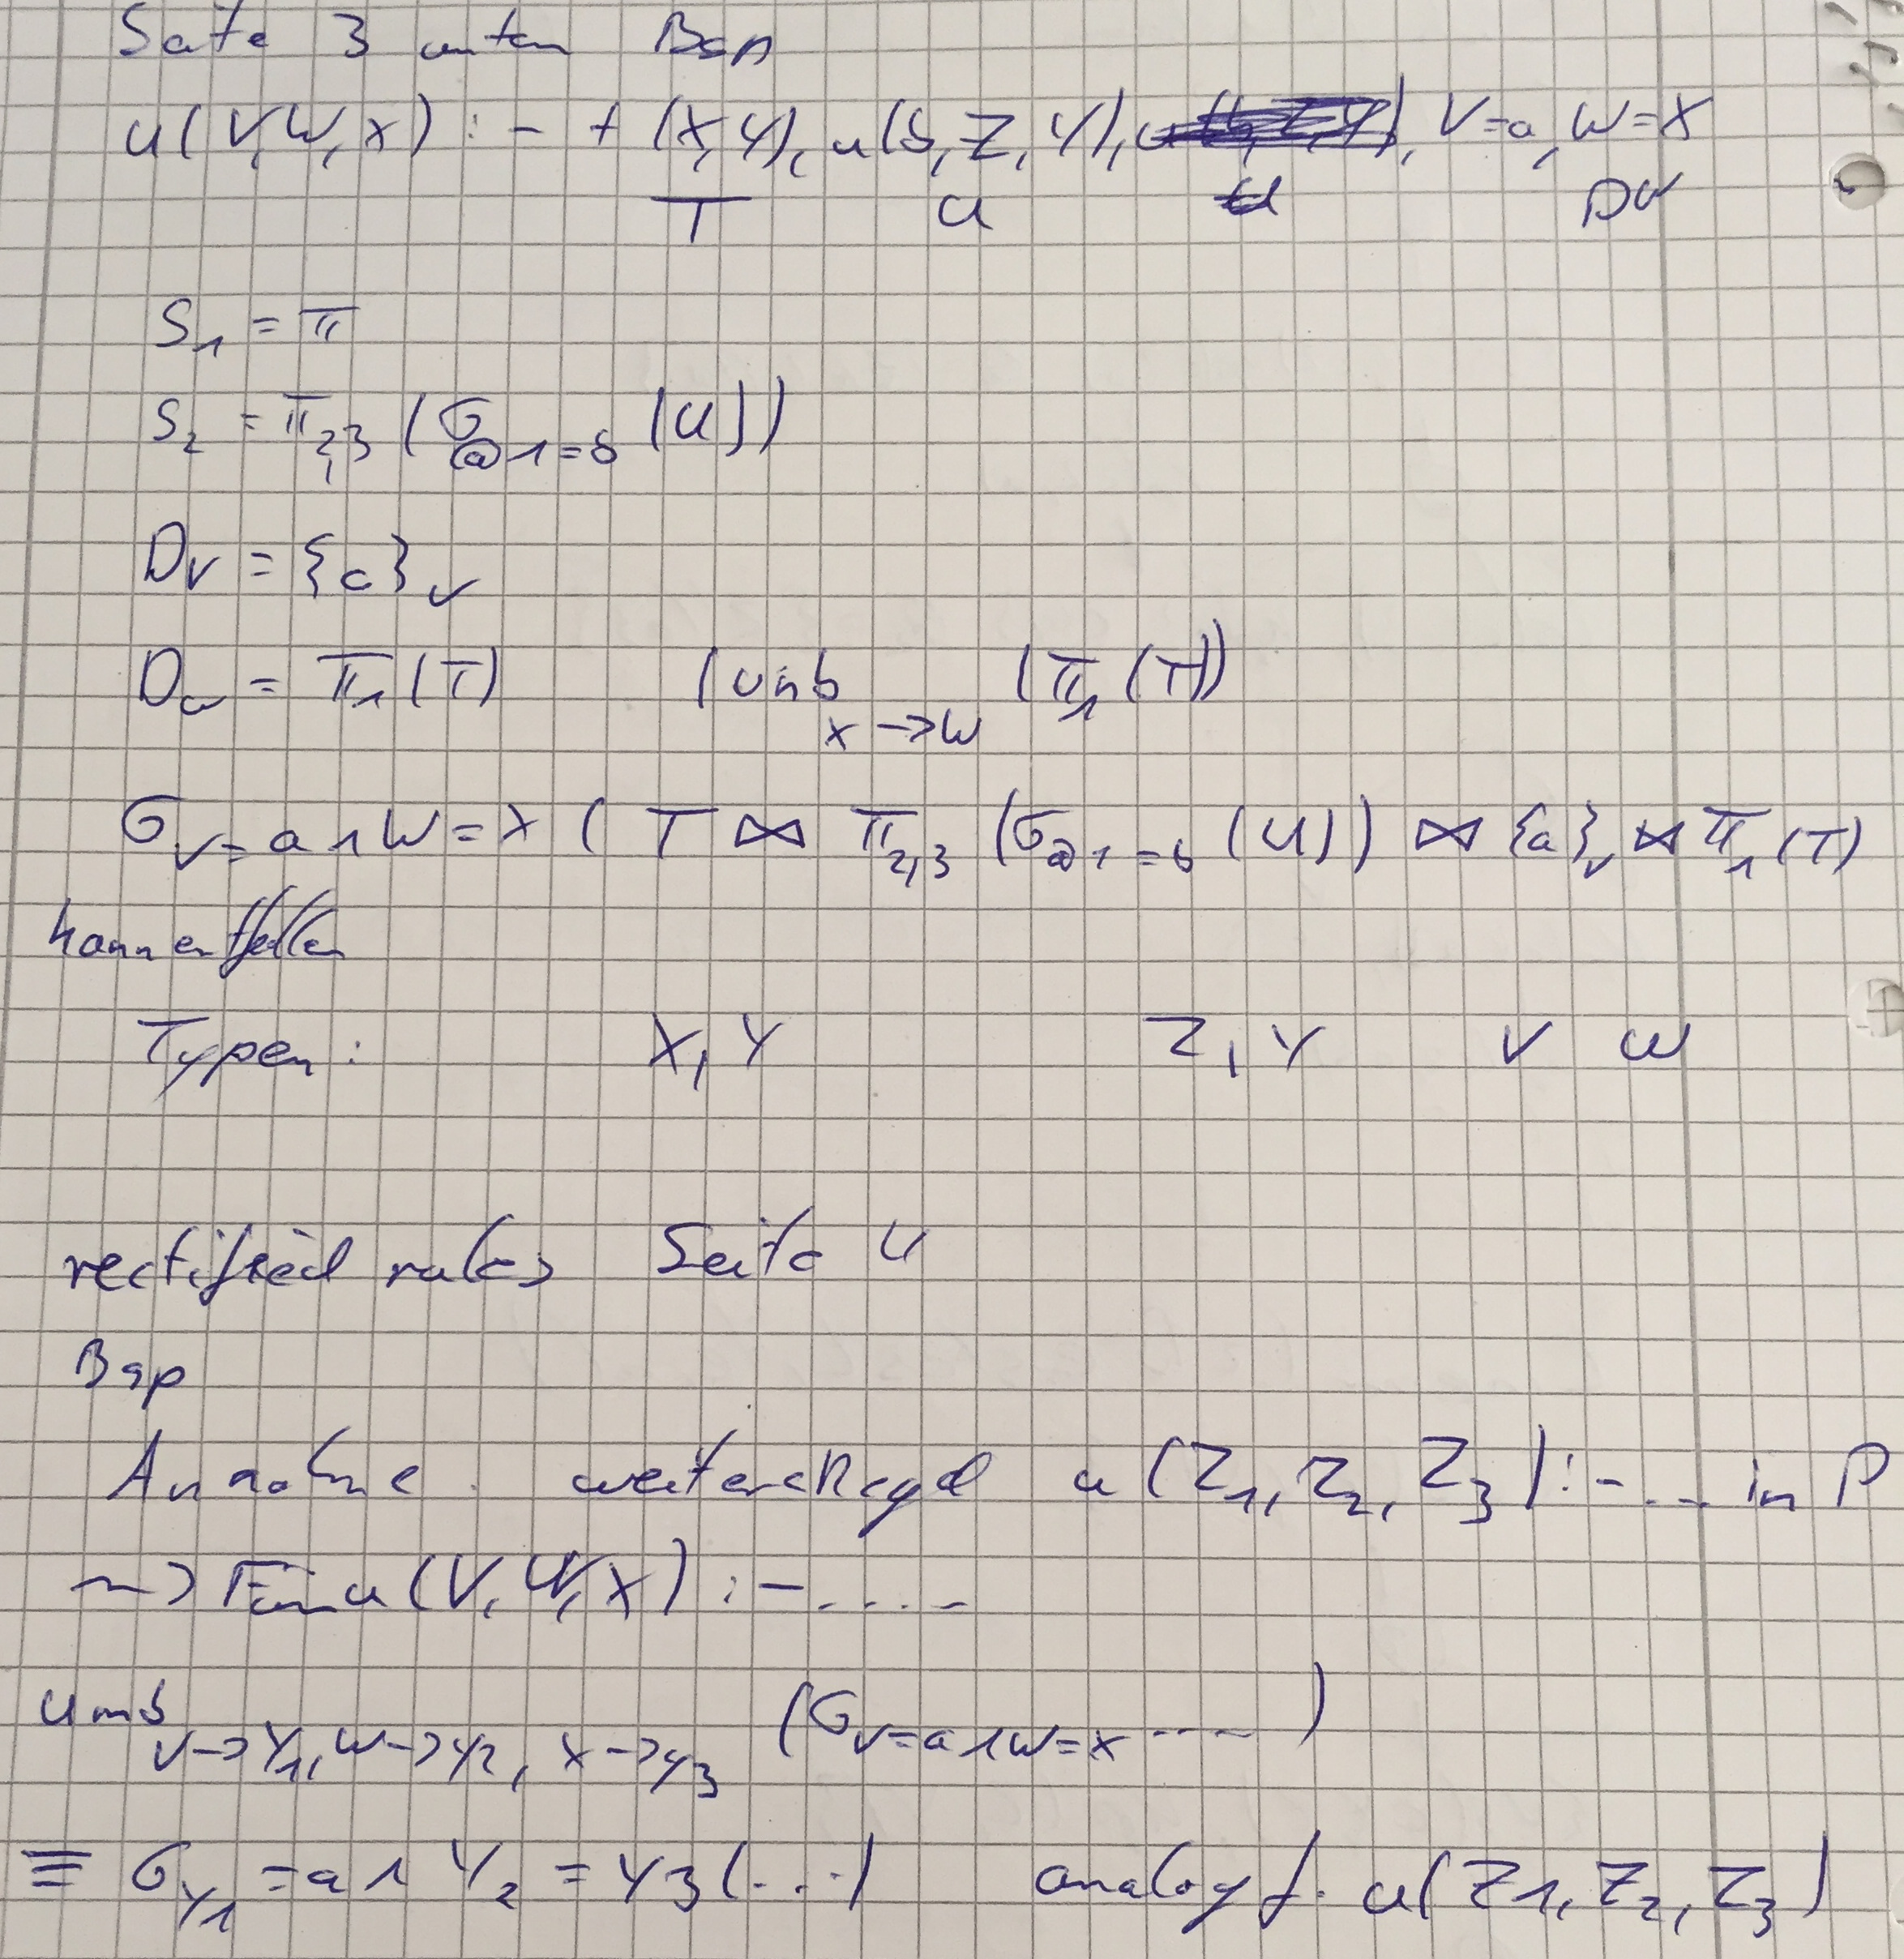
\includegraphics[width=0.7\linewidth]{img/img11}
\caption{}
\label{fig:img11}
\end{figure}
\end{itemize}


\paragraph{Beispiel} m alle Kurse $\neq$ a3 mit ihren Studierenden, die Voraussetzung von c4 sind.

\begin{align*}
r_1 = &vs(X,Y) :- Kp(X,Y). \\
&vs(c4, Y) :- vs(v4,Z), Kp(Z,Y). \\
&m(Z,W) :- vs(c4,Z), ag(Z,X), bl(Z,W,U), Z \neq a3.
\end{align*}

\paragraph{1.Schritt}
\begin{itemize}
\item $r_1$ \checkmark
\item $r_2 \leadsto \tilde{r_2} = vs(Q,Y) :- vs(C4,Z), kp(Z,Y), Q = c4.$
\item $r_3$ \checkmark
\end{itemize}

\paragraph{2.Schritt}
\begin{itemize}
\item $E_{r_1}$ = KURSPLAN
\item $E_{r_2} = \sigma_{Q = c4} \underbrace{\Pi_2 (\varsigma_{@1 = c4}(VS)}_Z \bowtie\footnote{Join Operation} \underbrace{KURSPLAN}_Z,Y \bowtie \underbrace{\{c4\}_Q)}_Q$
\item $E_{r_3} = \sigma_{Z \neq a3} \underbrace{\Pi_2 (\varsigma_{@1 = c4}(VS)}_Z \bowtie ANGEBOT \bowtie BELEGUNG$
\end{itemize}

\paragraph{3.Schritt}
vereinfacht $Q \Rightarrow X$\footnote{kommt nicht im Rumpf von $\tilde{r_2}$ vor}, damit $\tilde{r_1}$ und $\tilde{r_2}$ passen.
\begin{align*}
&vs(X,Y) \\
&vs(X,Y) \\
&m(Z,W)
\end{align*}


\paragraph{4.Schritt}
\begin{align*}
&VS = \underbrace{KURSPLAN}_{X Y} \cup \underbrace{(\Pi_2 (\varsigma_{@1 = c4}(VS)) \bowtie KURSPLAN \bowtie \{ c4 \}_X)}_X Y \\
&M = (\varsigma_{Z \neq a3}(\Pi_2 (\varsigma_{@1 = c4}(VS)) \bowtie ANGEBOT \bowtie BELEGUNG))[z,w]
\end{align*}

\subsubsection*{Schreibweise für Gleichungssysteme}

\begin{align*}
&R_i = E_i \underbrace{(R_1, \cdots, R_n)}_{DB-Relationen}, i = 1, \cdots, n
\end{align*}


Vergleich der Ausruckskraft\footnote{genauere Definition später} von Datalog und Relationale Algebra:

\begin{itemize}
\item Reines Datalog ohne Rekursion entspricht $RA^+$ (monotone Relationale Algebra)
\item Reines Datalog ohne Rekursion entspricht $RA^+$ ohne Gleichungssysteme (> $RA^+$)
\end{itemize}

\paragraph{Beispiel:}

Kursplan (kp): \\
\begin{tabular}{|c|c|}
\hline
X & Y\\ \hline
c4 & a3 \\
a3 & c2 \\
c4 & a2 \\
c2 & a0 \\
\hline
\end{tabular}


\begin{align*}
&vs(X,Y) :- Kp(X,Y).
&vs(X,Y) :- \underbrace{vs(X,Z)}_{X Z}, \underbrace{kp(Z,Y)}_{Z Y}.
&\leadsto vs = \Pi_{1,3}(VS \bowtie KURSPLAN) \cup KURSPLAN
\end{align*}

Jacobs entspricht Gauss-Seidel

\begin{align*}
R^0 &= \emptyset \\
Q^1 &= \emptyset \\
R^1 &= KP \quad \leftarrow (\emptyset_{X2} \bowtie KP_{ZY}) [X,Y] \\
Q^2 &= KP \\
R^2 &= \{ (c4,c2), (a3,a0) \} \cup KP \quad (KP_{XZ}) \bowtie KP_{ZY})[X,Y] \cup KP_{X,Y} \\
Q^3 &= R^2 \\
R^3 &= \{(c4,a0)\} \cup R^2 \quad (((KP_{XZ} \bowtie KP_{ZY}\footnotemark)[X,Y] \cup KP_{XY})_{XZ})[X,Y] \cup KP_{XY}  \\
\end{align*}
\footnotetext{Es wird zu viel berechnet beim Join. Siehe unten}
\subsubsection*{Anmerkung}
Berücksichtigung der ``neuen'' Information für VS hätte genügt. Grund: $(VS' \cup VS'') \bowtie KURSPLAN = VS' \bowtie KURSPLAN \cup VS'' \bowtie KURSPLAN $

\paragraph{Nach Schritt 4}

\begin{align*}
&R_1 \bowtie R_2 \cup R_2 \bowtie R_3 \Rightarrow^{mit \delta - Beruecksichtigung} \footnotemark \\
& \delta R_1 \bowtie \cup R_2 \bowtie R_3 \cup R_1 \bowtie \delta R_2 \cup \delta R_2 \bowtie R_3 \cup R_1 \bowtie R_2 \cup R_2 \bowtie \delta R_3 \\
&\Rightarrow\footnote{Ist besser} \delta R_1 \bowtie R_2 \cup R_1 \bowtie \delta R_2 \cup \delta R_2 \bowtie R_3 \cup R_w \bowtie \delta R_3
\end{align*}
\footnotetext{Ist suboptimal, weil wieder zu viel brerchnet wird}

\begin{align*}
& \delta R^0 = KP \\
& R^0 = KP \\
& \delta Q^1 = KP \\
& \delta R^1 = \{ (c4,c2), (a3,a0)\} \cup KP \\
& \delta R^1 = \{ (c4,c2), (a3,a0)\} \cup KP \\
& R^1 = Kp \cup \{(c4,c2), (a3,a0)\} \\
& \delta Q^2 = \{(c4,c2), (a3,a0)\} \\
& \delta R^2 =  \delta Q^2 \bowtie Kp \cup Kp = \{(c4,a0)\}  \cup Kp \\
& R^2 =  Kp \cup \{ (c4,c2), (a3,a0) \} \cup \{(c4,a0)\} \\
& \delta Q^3 = \{(c4,a0)\} \\
& \delta R^3 = \delta Q^3 \bowtie Kp \cup Kp = Kp \\
& \delta R^3 = \emptyset \\
& R^3 =  R^2 \cup \emptyset
\end{align*}

\begin{figure}[h!]
\centering
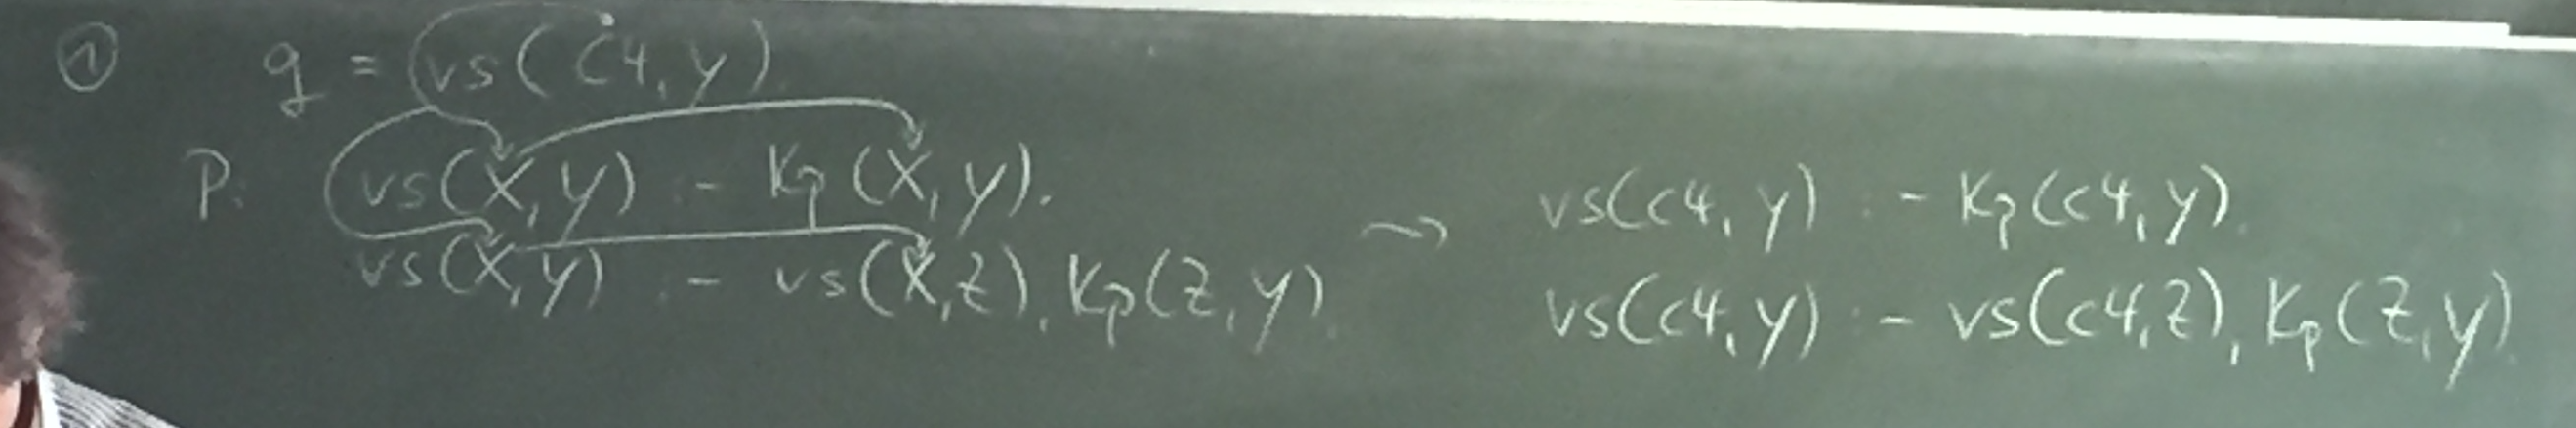
\includegraphics[width=0.95\linewidth]{img/img12}
\caption{}
\label{fig:img12}
\end{figure}

\begin{figure}[h!]
\centering
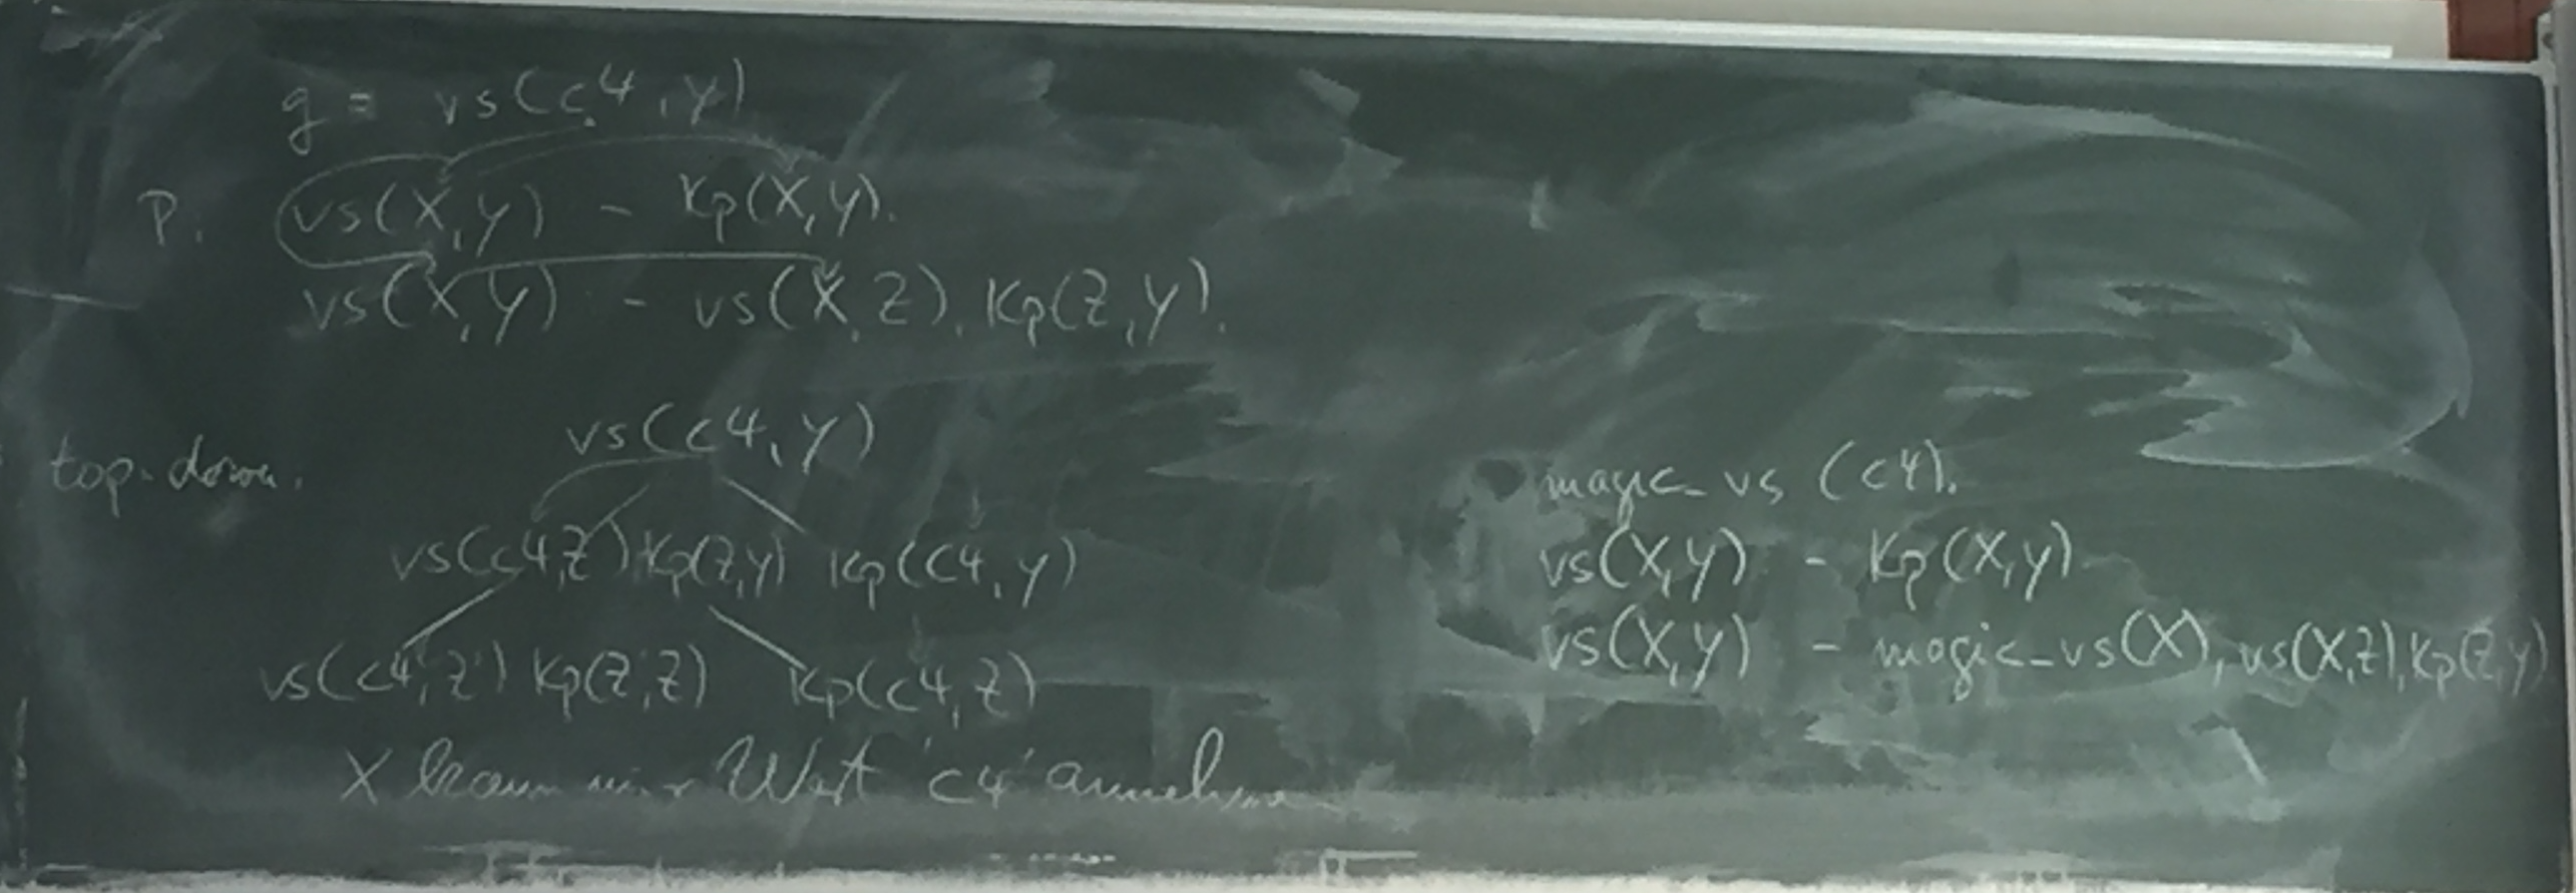
\includegraphics[width=0.95\linewidth]{img/img13}
\caption{}
\label{fig:img13}
\end{figure}

\begin{figure}[h!]
\centering
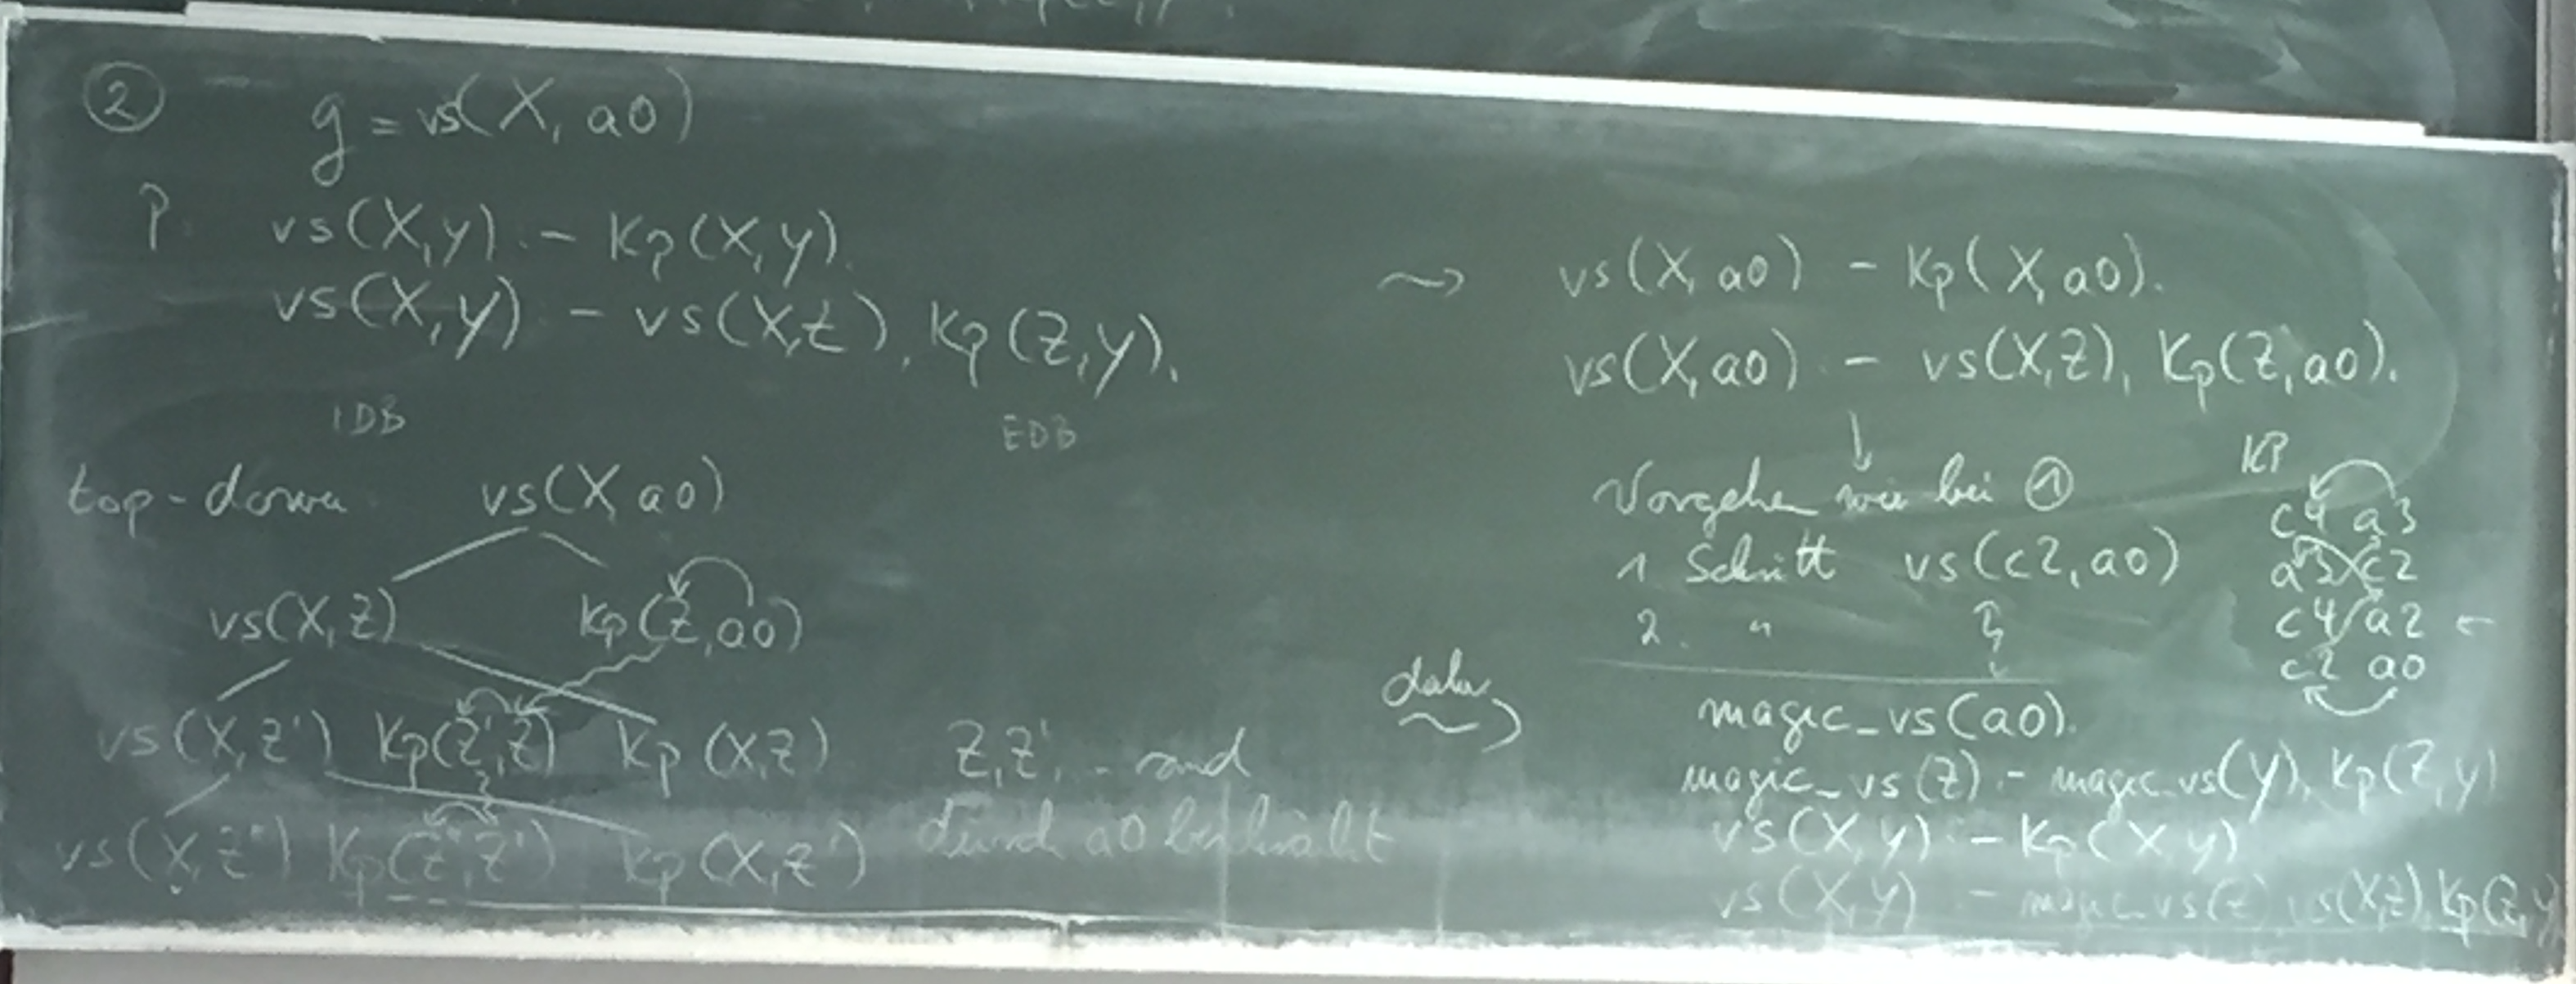
\includegraphics[width=0.95\linewidth]{img/img14}
\caption{}
\label{fig:img14}
\end{figure}

\paragraph{Beispiel}

\begin{align*}
&r_2 = vs^{fb}(X,Y) :- vs^{fb}\_(X,Z), Kp(Z,Y). \\
&i) \checkmark \\
&ii) \cdots magic\_r_2\_vs^{fb}\_1(X,Z) \cdots \\
&iii) \cdots magic\_r_2\_vs^{fb}\_1(Z) \cdots \\
&iv) vs^{fb}(Y)\\
& magic\_r_2\_vs^{fb}\_1(Z) :- magic\_vs^{fb}(Y), kp(Z,Y).
\end{align*}


\begin{align*}
&r_0 = query^f(X :- vs^{fb}\_(X,a0). \\
&i) \cdots \\
&ii) query^f(X) :- magic\_r_0\_vs^{fb}\_1(X,a0) \\
&iii) query^f(X) :- magic\_r_0\_vs^{fb}\_1(a0) \\
&iv) - \\
&v) vs^{fb}(Y)\\
& magic\_r_0\_vs^{fb}\_1(a0) :- magic\_query^f().\\
r_0 &\leadsto\footnotemark magic\_r_0\_vs^{fb}\_1(a0) :- . \\
r_2 &\leadsto magic\_r_2\_vs^{fb}\_1(Z) :- magic\_vs^{fb}(Y), Kp(Z,Y).
\end{align*}
\footnotetext{``Sideways information passing''}

\begin{align*}
&p(X):- \lnot q(X) \\
&p(X) \cup q(X) \\
&q(X) :- \lnot p(X)
\end{align*}

$P = \{ ag(a3, o) :- \lnot ag(a3,m) \}.$ \\
``Falls `m' Kurs a3 nicht anbietet, bietet o den Kurs an'' \\
Mit CWA: 

\begin{align*}
&ag(a3,m) \not\in ANGEBOT \\
&ag(a3,o) \not\in ANGEBOT
\end{align*}

Da beide keine logische Folgerung von P (müsste in allen Modellen gültig sein) Nimm Modelle $\{ ag(a3, o) \}$.

\begin{align*}
&\{ ag(a3, o) \} \\
& \Rightarrow^{CWA\footnotemark} \lnot ag(a3, m) \text{ und } \lnot ag(a3, o) \text{ sind gültig.} \\
& \text{Aber } \lnot ag(a3,m) \Rightarrow ag(a3,0) \leadsto \text{Wiederspruch zur CWA}
\end{align*}
\footnotetext{Closed World Assumption}

Beachte folgende HB-Interpretation von P.

\begin{align*}
&I_1 = \{ ag(a3, o) \} \text{ und } I_2 = \{ ag(a3, m) \} (I_1, I_2 \text{ sind minimale Modelle}) \\
&I_3 = \{ ag(a3, o), ag(a3,m) \} \text{ ist ebenfalls Modell von P}
\end{align*}

In $I_1$ gilt mit CWA: $\lnot ag(a3,m)$ \\
In $I_2$ gilt mit CWA: $\lnot ag(a3,o)$ \\

\paragraph{Grund für Problem:} Implikation $\lnot ag(a3,m) \Rightarrow ag(a3, o)$ äquivalent zu $ag(a3,m) \vee ag(a3, 0)$. Welches Modell soll ausgezeichnet werden? Semantik?

\paragraph{Offensichtlich:} I Modell von P $\diamondsuit$ I Modell von $P' = \{ ag(a3,m) :- ag(a3, o)\}$
Gehe wie bei Fuxpunktberechnung vor:

\paragraph{P}
Bekannte Fakten $EDB = \{ ag(a1,m)\, ag(c4,q), ag(a3,d), \cdots \}$ \\
$ag(a3, m) \not \in EDB$ \\
CWA: $\lnot ag(a3, m) \text{ gilt} \Rightarrow^{\text{Regel}} ag(a3,0)$ \\

\paragraph{P'}
$ag(a3, o) \not \in EDB$ \\
CWA: $\lnot ag(a3, 0) \text{ gilt} \Rightarrow^{\text{Regel}} ag(a3,m)$ \\

Daraus folgt: Wähle $I_1(I_2)$ als Modell (Semantik) von P(P') $\leadsto$ Auswertungsrichtung gemäß Implikation legt Semantik fest. D.h. Semantik ist abhängig von der Art des Aufschreibens der Klauseln. Daraus ergibt sich die Frage nach einer besseren Semantikdefinition.

\begin{figure}[h!]
\centering
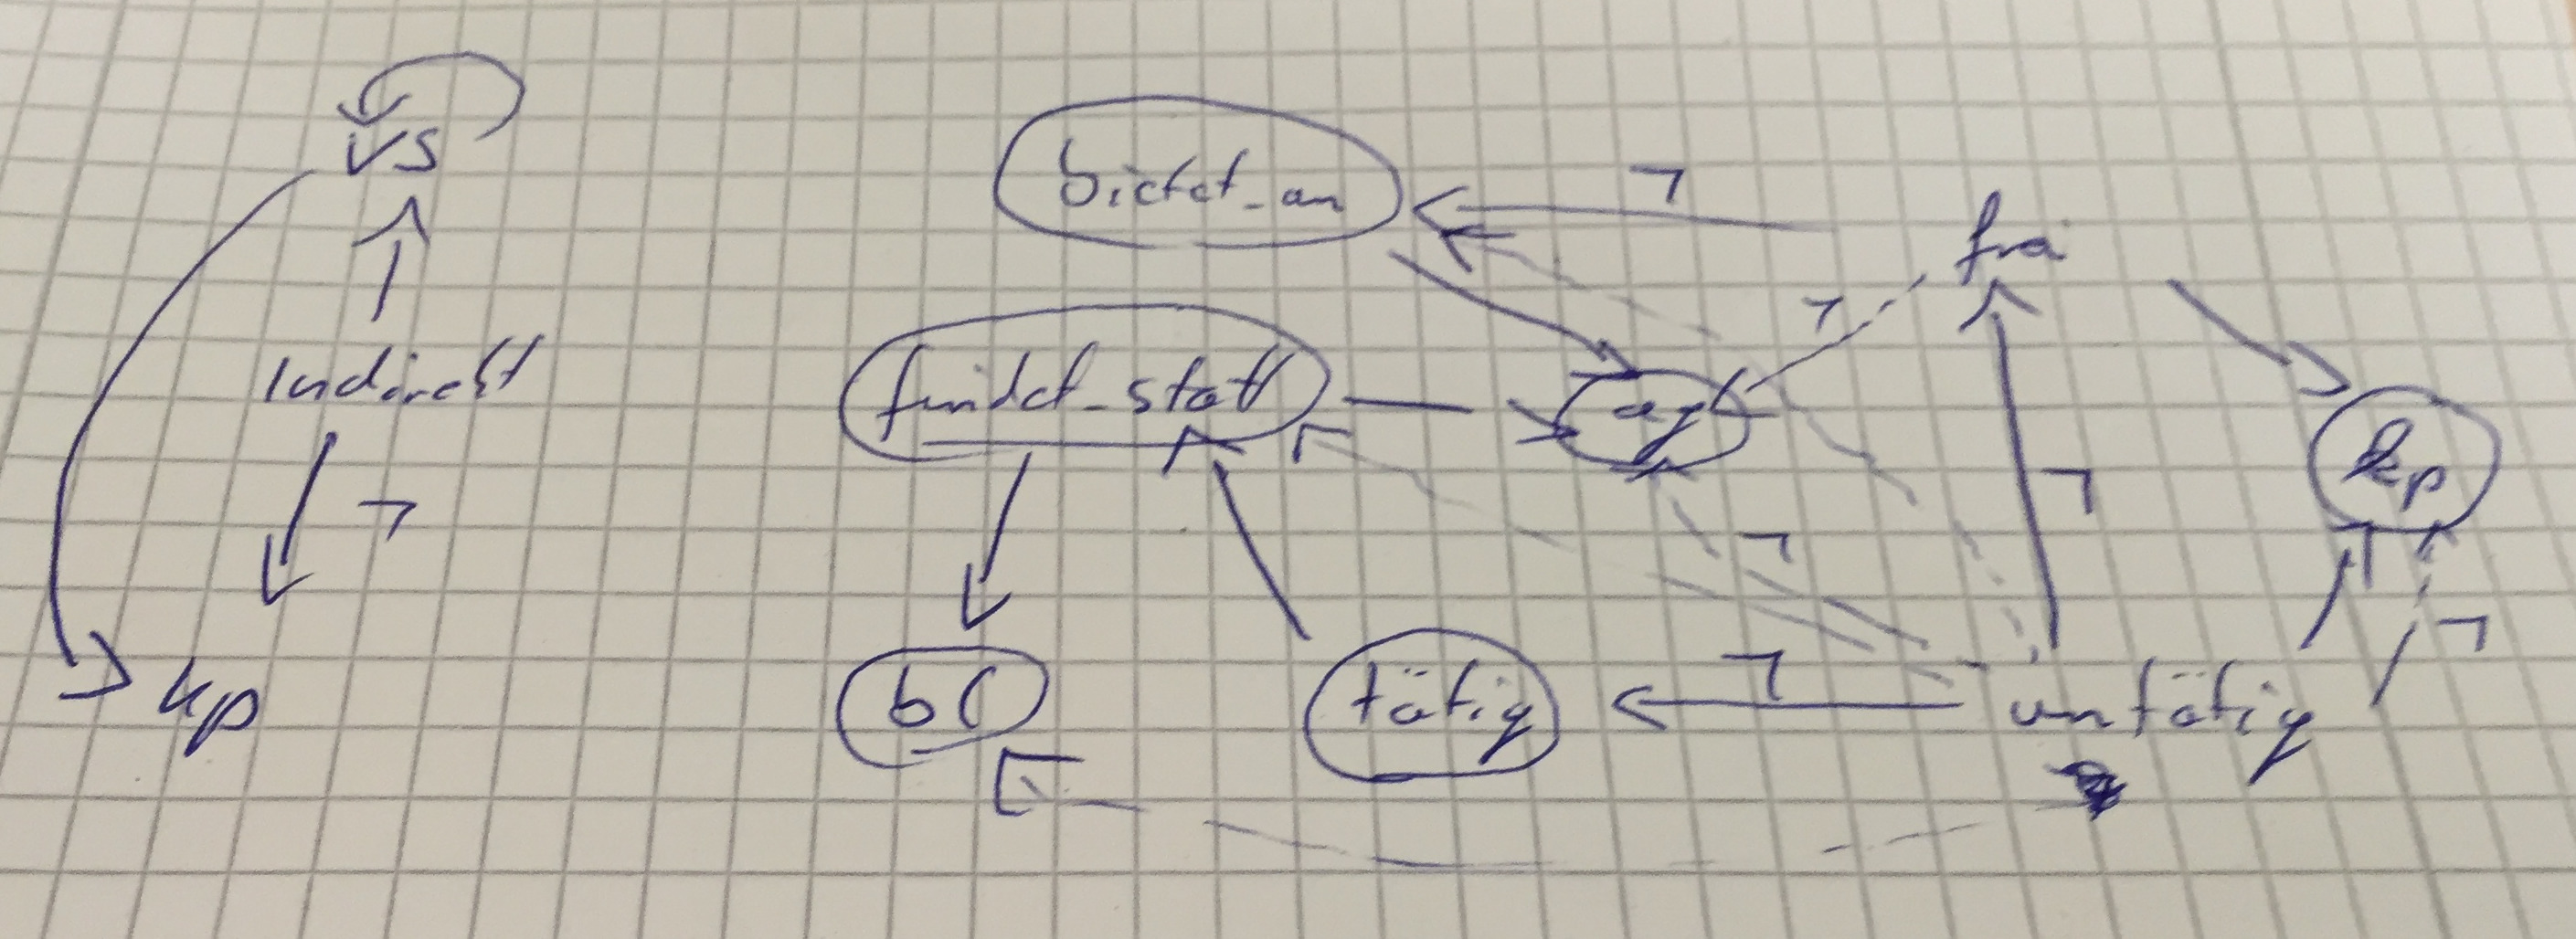
\includegraphics[width=0.95\linewidth]{img/img15}
\caption{}
\label{fig:img15}
\end{figure}

\begin{align*}
r(1), s(1), s(2).& \\
U(X) :- r(X). r(1) \leadsto u(1)& \\
q(X) :- s(X), \lnot u(X).& \Leftarrow s(1) \leadsto q(1)\\
& \Leftarrow s(2) \leadsto q(2)
\end{align*}

\subsection*{Disjunktives Datalog}
Einige Bermerkungen zu disjunktivem Datalog. Negationen im Rumpf sind umgeschrieben genau ein Oder (Disjunktion).

Form 6: $q_1(\cdots), \cdots, q_n(\cdots) :- p_1(\cdots), \cdots, p_n(\cdots).$

Negation in Rümpfen erlaubt $\Rightarrow$ Frage: Sind Disjunktionen im Kopf von Regeln notwendig? \\

\paragraph{Beispiel:}  
Tim ist 18 oder\footnote{Altagserfahrung: Exklusiv, Theoretisch liegt dieses Wissen um exklusivitöt nicht vor.} 16 Jahre alt: $alter(tim, 18), alter(tim, 16) :- .$

Logisch äquivalent zu: \footnote{Tim ist 18 oder 16 Jahr alt, mehr wissen wir nicht (oder formal gesehen inklusives Oder)}
\begin{align*}
&alter(tim, 18) :- \lnot alter(tim, 16). \\
&alter(tim, 16) :- \lnot alter(tim, 18). \footnotemark
\end{align*}
\footnotetext{Tim ist 18 Jahre alt, wenn er nicht 16 Jahre alt ist}
$\leadsto$ Falls auf ``Tim ist nicht 18 Jahre alt.'' etwas mit CWA geschlossen werden kann, folgt definitiv ``Tim ist 16 Jahre alt.''.\\
Mehrere Semantiken in Literatur vorgelschlagen, etwa:

\subsubsection*{``General Closed World Assumption'' (GCWA)}
\paragraph{Idee:}
Weil mehrere minimale Herbrand Modelle möglich sind $\leadsto$ Schluss auf das Negaitve, $\lnot p$, genau dann möglich wenn $p$ in keinem minimalen Modell enthalten ist.

\paragraph{Beispiel:} $\{ alter(tim, 18) \}, \{ alter(tim, 16) \}$ sind die beiden minimalen Modelle \\
$\{ alter(tim, 18), alter(tim, 16) \}$ ist auch ein Modell, aber nicht minimal. \\

Minimale Modelle: $\{ q,r \}, \{q,s \}$
\begin{align*}
P = \{ p,q :-.& \\
q :- . & \\
r,s :-.& \}
\end{align*}

p ist in keinem minimalen Modell enthalten $\leadsto \lnot p$  kann unter GCWA angenommen werden.

\paragraph{Eigenschaften}
GCWA erfüllt die Eigenschaften der

\begin{itemize}
\item + Konsistenz: Negative Information, die auf Grund der GCWA hinzugefügt wird, führt nicht zu Widerspruch in der Theorie.
\item + Stabilität: Negative Information, die auf Grund der GCWA hinzugefügt wird, verringert die positive Information nicht und vergrößert sie auch nicht.
\item + Reduktion: Für definite Programme entspricht die GCWA der CWA. 
\item - Monotonie: CWA garantiert Monotonie, GCWA nicht.
\end{itemize}

\subsubsection*{Monoton}
Seien P,P' definite oder disjunkte Programme. Sei R eine Negationsregel mit R(P) definiert die Menge der negativen Atome, die gemäß R für P angenommen werden können. \\
R ist monoton $\diamondsuit P \subseteq P' \Rightarrow R(P') \subseteq R(P)$  

\paragraph{Beispiel}

\begin{align*}
&P =  \{ p(a) \vee p(b) \} \\
&P' = P \cup \{ p(a) \} \\
&P'' = P' \cup \{ p(b) \}
\end{align*}

Success:
\begin{align*}
&\text{Success von }P =  \{ p(a) \vee p(b) \} \\
&\text{Success von }P' = \{ p(a) \vee p(b), p(a) \} \\
&\text{Success von }P'' = \{ p(a) \vee p(b), p(a), p(b) \}
\end{align*}

Unknown:
\begin{align*}
&\text{Unknown von }P =  \{ p(a), p(b) \} \\
&\text{Unknown von }P' = \emptyset \\
&\text{Unknown von }P'' = \emptyset
\end{align*}

Mit GCWA:
\begin{align*}
&\text{Durch GCWA von }P =  \emptyset \\
&\text{Durch GCWA von }P' = \{ \lnot p(b) \} \\
&\text{Durch GCWA von }P'' = \emptyset
\end{align*}

Dadurch ist zu sehen, dass die Monotonie verletzt (zwischen P' und P''), damit ist die GCWA nicht monoton.


\begin{figure}[h!]
\centering
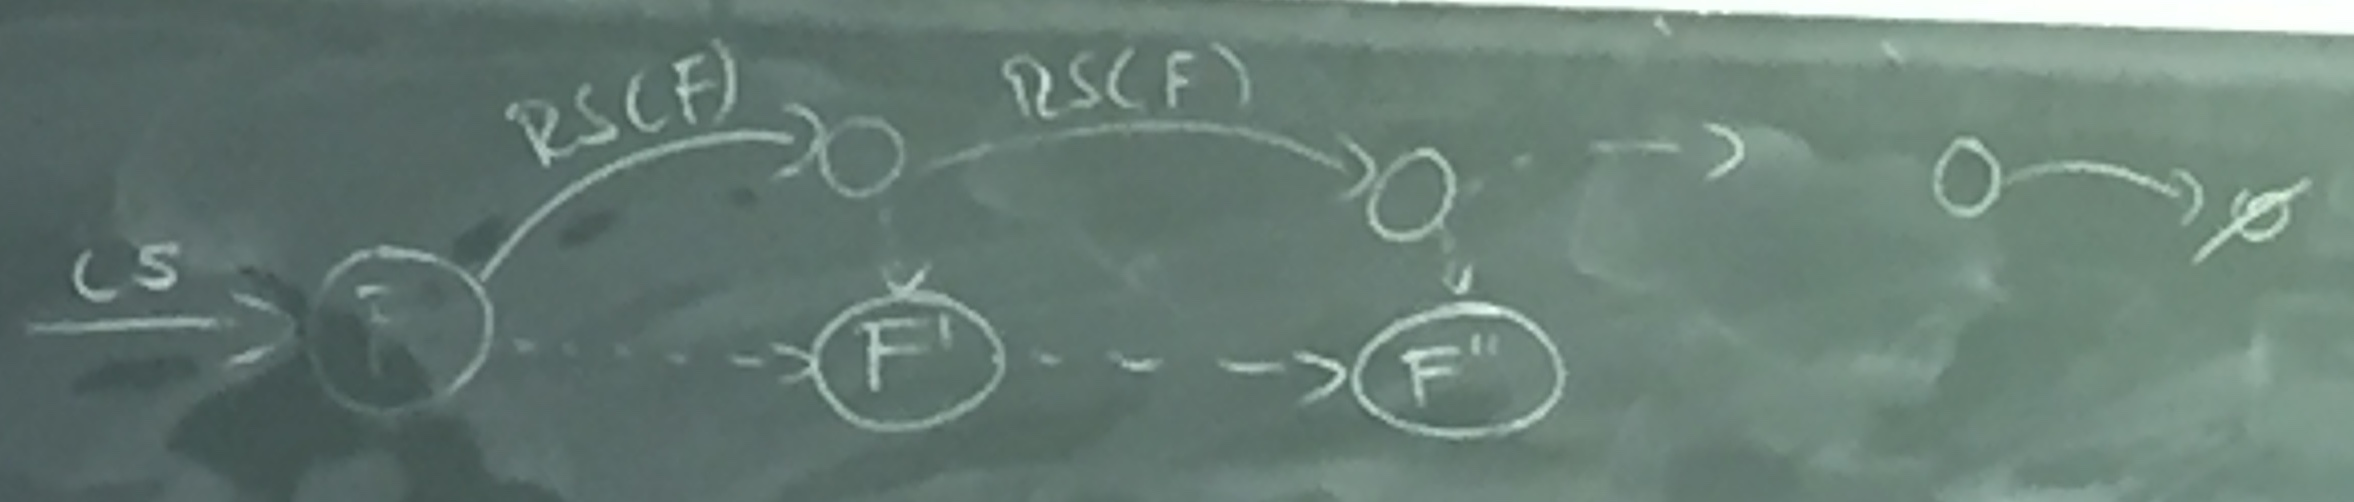
\includegraphics[width=0.95\linewidth]{img/img16}
\caption{}
\label{fig:img16}
\end{figure}


\begin{align*}
& ANCESTRY(X,Y) :- MOTHERHOOD(X,Y). \\
& ANCESTRY(X,Y) :- MOTHERHOOD(X,Z), ANCESTRY(Z,Y). \\
\end{align*}


\begin{figure}[h!]
\centering
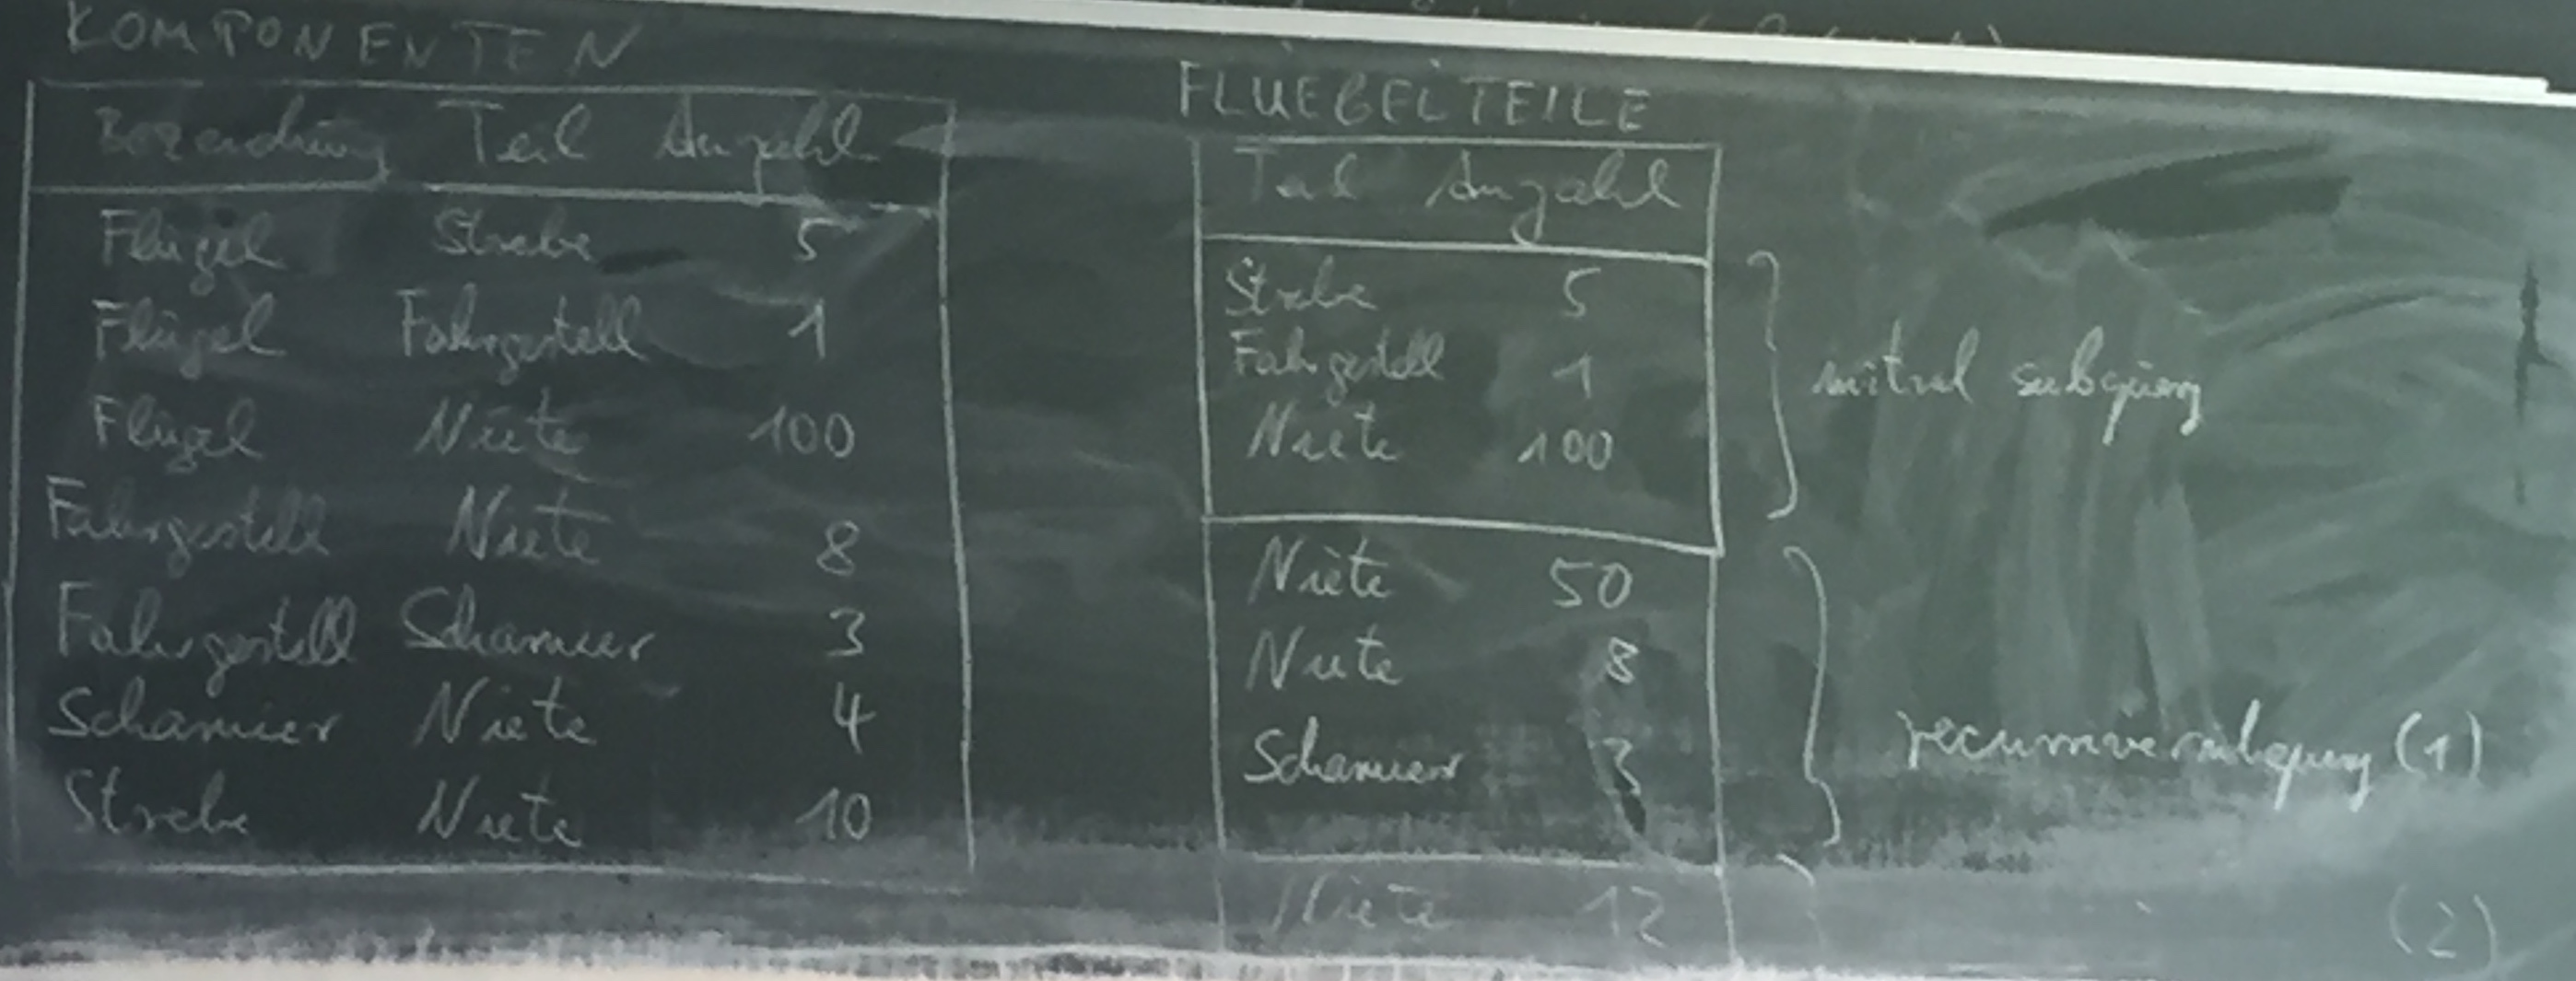
\includegraphics[width=0.95\linewidth]{img/img17}
\caption{}
\label{fig:img17}
\end{figure}

\subsection*{Rekursion in SQL}

Flüge: \\
\begin{tabular}{|c|c|c|c|}
\hline
Flugnr. & Ab & Ziel & Kosten \\ \hline
LH577 & FRA & JSK & 700 \\
RA170 & LHR & JFK & 400 \\
LH122 & HAM & FRA & 100 \\
BA730 & FRA & LHR & 150 \\ 
... & ... & ... & ... \\
\hline
\end{tabular}

Reisen: \\
\begin{tabular}{|c|c|c|}
\hline
Ziel & Route & Gesamtkosten \\ \hline
fra & ``fra'' & 100 \footnote{Initial Subquery} \\
\hdashline
jfk & ``FRA,JFK'' & 800\footnote{Recursive Subquery (1)} \\
lhr & ``Fra,lhr'' & 250\footnote{Recursive Subquery (1)} \\
\hdashline
jfk & ``fra,lhr,jfk'' & 650\footnote{Recursive Subquery (2)} \\
... & ... & ...  \\
\hline
\end{tabular}

\subsection*{Negation in SQL}
(except \& not) \\

\paragraph{Forderung}: Stratifikation
\paragraph{Beispiel}: Gegeben DAG(K1, K"). Gesucht Paare von Knoten, die nur mit Pfade in gerader Länge verbunden sind.
\paragraph{1.Ansatz}
\begin{lstlisting}[language=SQL]
with recursive UAB(K1, K2) as 
((select * from DAG)
  union 
  (( select d.K1, g.k2
     from DAG d, GAB g 
     where d.K2 = g.K1)
    except
      (select * from GAB))),
      GAB(K1, K2) as (select d.K1, UAB u where d.K2 = u.K1) 
      ))
\end{lstlisting}
\footnote{GAB noch nicht bekannt}

\paragraph{Uniformulieren}

\begin{lstlisting}[language=SQL]
with recursive UAB(K1, K2) as
  ((select * from DAG)
    union 
    ((select d.K1, u.K2 from DAG d, DAG d1, UAB u
      where d.K2 = d1.K1 and d1.K2 = u.K1)
      except
        (select * from GAB))),
        GAB(K1, K2) as ((select d.K1, d.K2 from DAG d, DAG d1 
          where d.K2 = d1.K1)
          union
          (select d.K1, g.K2 from DAG d, DAG d1, GAB g
            where d.K2 = d1.K1 and d1.K2 = g.K1))
    )
  )
select x from UAB;
\end{lstlisting}

\section*{2: Ausdruckskraft und Komplexität von Anfragesprachen}

Ausdruckskraft infromell: Welche Information kann mit Hilfe der Anfrage der Spracha sue einer beliebigen Datenbank ermittelt werden.

\subsection*{Formalisierung für relationale Datenbanken}
\subsubsection*{Definition: Anfrage}
Sei $\sigma = \{ (RT_1, \alpha_1), \cdots, (RT_nm \alpha_n) \}$ ein relationales Datenbankschema über $\alpha = \bigcup^n_{i = 1} \alpha_i$ mit Wertebereichsfunktion dom. Sei $\alpha$ in eine genügend große Attributmenge $\alpha_0$ eingebettet\footnote{Enthalten darin}. \\
Eine Anfrage q auf $\sigma$ ist eine partielle Funktion
\begin{align*}
q | Z \sigma \Rightarrow R^{\infty}_{\beta}
\end{align*}

dabei gilt $\beta \subseteq \alpha_0$ und $R^{\infty}_{\beta}$ ist die Menge der verallgemeinerten DB-Relationen über $\beta$. (unendliche Tupelmenge erlaubt)

\subsubsection*{Definition: Anfragesprache}
Eine Anfragesprache zu $\sigma$ ist eine Menge $L_0$ von Ausdrücken zusammen mit einer Bedeutungsfunktion (in Zeichen: $(L_{\sigma}\footnote{Sprache}, \mu\footnote{Bedeutungsfunktion})$), so dass für jeden Ausdruck $e \in L_{\sigma}$ gilt: $\mu(e) \text{ ist eine Anfrage von } \sigma$ 

\subsubsection*{Definition: Ausdruckskraft}
Die Ausdruckskraft einer Anfragesprache $(L_{\sigma}, \mu)$ zu einer DB-Schema $\sigma$ ist definiert als $\mu(L_{\sigma}) =_{Def.} \{ \mu(e) | e \in L_{\sigma} \}$. Eine Sprache $(L_{\sigma}, \mu')$ ist \textbf{ausdrucksstärker} als eine Sprache $(L_{\sigma}, \mu)$, wenn gilt: $\mu(L_{\sigma}) \subseteq \mu'(L'_{\sigma})$
Im Fall $\mu(L_{\sigma}) = \mu'(L'_{\sigma})$ werden die Sprachen \textbf{äquivalent} genannt

\paragraph{Informell}
Welche Information können mit Hilfe der Anfragen der Spache aus einer beliebigen Datenbank ermittelt werden

\paragraph{Problem}
Information mit Algebra geht nicht: ``Die Mitarbeiter die über 10k verdienen sind grade die Manager''. Inrinsische Informationen stellen ein Problem dar.

\subsubsection*{Definition: Anfragesprache von $\rho$}
%TODO: Überprüfen wegen schlechter handschrift
Sei $\rho = \{ (RT_i, \alpha_i) | i \in Lm \}$ ein relationales Datenbankschema über $\alpha = \bigcup \alpha_i$ mit Werteberichsfunktion dom. Sei $\alpha$ in eine genügend große Attributmenge $\alpha_0$ eingebettet. Eine Anfrage q ist eine partielle Funktion mit $q: \delta_\rho \rightarrow R^{\infty}_\beta,  \delta \subseteq \alpha_0, R^{\infty}_\beta$ ist die Menge der verallgemeinerten DB-Relationen über $\beta$ (unendliche Teilmengen sind erlaubt). \\
Eine Anfragesprache zu $\rho$ ist eine Menge $L_\rho$ von Ausdrücken mit einer Bedeutungsfunktion $\mu$ (schreibe $(L_\rho, \mu)$), so dass für jeden Ausdruck $e \in L_\rho$ gilt $\mu(e)$ ist eine Anfrage an $\rho$.

\subsubsection*{Definition: Ausdruckskraft einer Anfragesprache von $\rho$}
Die Ausdruckskraft einer Anfragesprache $(L_\rho, \mu)$) zu $\rho$ ist definiert als $\mu(L_\rho) = \{ \mu(e) | e \in L_\rho \}$

\subsubsection*{Definition: Äquivalenz von Sprachen}
$(L'_\rho, \mu') = (L_\rho, \mu)$, wenn $\mu'(L'_\rho) = \mu(L_\rho)$. Kleiner und größer analog.
Falls Anfragesprache L für alle $\rho$ äquivalent zu Anfragesprache L' ist werden beide als äquivalent bezeichnet.

\subsubsection*{Vergleich Datalog - Relationenalgebra}
\begin{itemize}
	\item Reines Datalog ohne Rekursion \texttt{entspricht} $RA^+$ (monotone Relationenalgebra)
	\item Reines Datalog mit Rekursion \texttt{entspricht} RA Gleichungssysteme
	\item Datalog mit Negation ohne Rekursion \texttt{entspricht} RA
	\item volles Datalog \texttt{>} RA
	\item Datalog mit geschichteter Negation \texttt{<} Inflationäre Semantik
\end{itemize}

\subsubsection*{Berechenbarkeitsmodelle}
Alegraisch logische Definitionen
\begin{itemize}
	\item allgemein rekursiove Funktionen (Gödel / Herbrand 1936)
	\item $\lambda$-def. Funktionen (A. Church 1936) 
	\item $\mu$-rekursive Funktionen und partiell definierte Funktionen (Gödel / Kleene 1936)
\end{itemize}

\subsubsection*{Wortersetzungssysteme}
\begin{itemize}
	\item Turing Maschine (1936)
	\item Postsche Kanonische Systeme (1945)
	\item Markov-Algorithmen (1951)
\end{itemize}

\subsubsection*{Theoretische Berechnungsmodelle}
\begin{itemize}
	\item unbeschränkte Registermaschine (1963)
	\item Random Access Machine (1964)
\end{itemize}

\subsection*{Ausdruckskraft von Relationenalgebra und ???}
Grobe Charakterisierung der RA (ohne Erweiterung)
\begin{itemize}
	\item Operatoren können keine neuen Werte erzeugen, d.h. Werte in Ergebnissen müssen in Operanden auftauchen
	\item es können beliebige Relationstypen über den gegebenen Wertebereichen auftreten / erzeugt werden (Umbenennung)
	\item Für einen festen Datenbankzustand $\delta$ zu $\rho$ gilt: mit RA-Ausdrücken können alle Relationen erzeugt werden, die nur Informationen erhalten der schon in Z enthalten ist.
\end{itemize}

\paragraph{Operatoren:}  $\cup, \cap, \backslash, \bowtie,$ Projektion, Selektion (mit allg. Vergleichsausdrücken,  Division, Umbenennung)
\paragraph{Sonderstellung:} Komplement \\
Sei R eine DB Relation über $\beta$, $T_\beta$ sei die Menge aller DB-Tupel über $\beta$. R[kompl] = $T_\beta \backslash R $ (i.A. eine unendliche Tupelmenge)
\paragraph{Beispiel:} Noch offene Blätter für jeden angemeldeten

\subsubsection*{Satz 2.1}
Sei e ein zu einem gegebenen Datenbankschema $\rho$ passender RA-Ausdruck ohne Komplement. Dann gibt es einen äquivalenten zu e passenden Ausdruck der RA e' in dem als Operatoren nur Selektionen mit einfachen Vergleichsausdrücken, direktes Produkt, Projektion, Umbenennung, Differenz, Vereinigung vorkommen. Als Operanden ermittelt e' neben Relationstypbezeichnern aus $\rho$ nur (extensionale) DB-Relationen der Form $\{(A, C), A \in \alpha_\rho, c \in dom(A) \} $\\

Weitere Einschränkungen sind möglich $\rightarrow$ Projektionen nur auf ein Attribut, Vergleichsausdrücke = und >. \\
Falls Komplementbildung hinzugenommen, Differenz nicht mehr notwendig: \\
$R \backslash S = (R[kompl] \cup S)[kompl]$

\subsubsection*{Satz 2.2}
Eine derart ??? Operationsmenge der RA ist minimal, d.h. es kann keine Operation entfernt werden, ohne dass die Ausdruckskraft eingeschränkt ist.

\paragraph*{Beweisidee:} Diskutiere die speziellen Eigenschaften und zeige dass diese Operation über Eigenschaften verfügt, die keiner anderen Operation oder Kombination von Operationen zukommt. Z.B. Vereinigung: Streiche, Neuverknüpfung 2er Relationen dann nur noch über Differenz und direktes Produkt möglich. Vereinigung erlaub das hinzufügen eines neuen Tupels unter Attribut Kombination, direktes Produkt und Differenz nicht \\

Mit der Relationenalgebra kann nicht allgemein die transitive Hülle berechnet werden.

\subsubsection*{Satz 2.3}
Sei RT der Bezeichner eines beliebigen, zweistelligen Relationstyp über abzählbaren unendlichen Wertebereich. Sei Rt* der Relationstyp für die transitive Hülle von Relationen des Typs RT. Es gibt keinen Ausdruck  der Relationenalgebra mit der Eigenschaft $e(RT) ? = RT*$. \\

Gegeben Wertebereich $\{a_1, a_2, \cdots \}$ ohne Ordnungsrelation. Betrachte $R_l = \{ (a_i, a_i+1) | i \in [l-1] \}$ für $l \in \mathbb{N} \}$. $R_l$ ist eine mathematische Relation, die Tupel sind also geordnet. Zeige $e(R_l) \neq R*_l$ für jeden RA - Ausdruck e, der zu Wertebereichen passt und für genügend großes l. $e(R_l)$ bedeutet $R_l$ für RT eingesetzt. RA-Operationen sind anzupassen (wir haben keine Bezeichner $\leadsto$ Permutationen einführen) .
\begin{itemize}
	\item Projektion: \footnote{entspricht $\exists$: es gibt da was in der spalte, aber was das ist, ist mir egal} erlaubte Permutationen (vgl p(x) :- r(y,x) ist Projektion in r)
	\item Selektionen mit atomaren Vergleichsausdrücken der Form $i = a_m, i \neq a_m, i = j, i \neq j$ für $i,j \in [k], m \in [l]$ k ist bestimmt durch Größe der konstruierten Tupel $(b_1, \cdots, b_k), b_i \in \{a_1, \cdots a_l \}$
\end{itemize}

\subsection*{Beweis}

\begin{align*}
&R_l = \{(a_1, a_2), (a_2, a_3), \cdots, (a_{l-1}, a_l) \} \\
&e(R_l) = R_l^+
\end{align*}

Einfache Erweiterung, um Hüllenberechnung zu ermöglichen: \\
Erlaubte Gleichungen (vgl. Datalog-Übersetzung) der Form 
\begin{align*}
&RT = f(RT) \\
&(RT, \{ A_1, \cdots, A_k \}), \{ A_1, \cdots, A_k \} \subseteq \alpha_0 \\
& RT \in \{ RT_1, \cdots, RT_m \}
\end{align*}

\paragraph{$f(RT):$} RA-Ausdruck, der bis auf RT zu $\sigma$ passt, und der nicht die Differenz enthält ($\leadsto$ monoton).
\paragraph{Beispiel}: Sei $(S, \{A, B \})$ ein binärer Relationstyp und o die Komposition von Relationen mit Darstellung $R_1 o R_2 = (R_1 \bowtie R_2)[1,4]$.

\paragraph{Hülle von S:} kleinster Fixpunkt von $R = R o S \cup S$. \\
Berechnung (Fixpunktsatz): $f^{m_0}(\emptyset) = \bigcup^{\infty}_{i = 1} S o \cdots o S\footnote{i-Mal}$, $m_0$ Zahl mit $f^{m_0})(\emptyset) = f^{m_0 + 1}(\emptyset)$ 
 

\paragraph{Selektionen:}
\begin{align*}
i = a_m \quad i \neq a_m \quad i = j \quad i \neq j
\end{align*}

Andere Formen sind nicht von Interesse, da Werebereich ohne Ordnungsrelation und ohne spezielle Operationen festgelegt. Z.B. nicht möglich $(R_l[1] \bowtie R_l[2])[ 2 > 1]$.
Elemente Operatorn in RA-Ausdrücken, die zu RT passen:
\begin{itemize}
\item RT
\item endl. Teilmenge des Wertebereichs
\end{itemize}


Betrachte Kalkülausdruck der Form $\{ (X_1, \cdots, X_K) / \Psi(X_1, \cdots, X_k) \}$ mit folgenden Vergleichsausdrücken:
\begin{itemize}
\item $X_i = a_m,\quad X_i \neq a_m$
\item $X_i = X_j \uparrow c,\quad X_i \neq X_j \uparrow c, \quad c \in \mathbb{Z} \text{ beliebig, mit Interpretation } (b_1, \cdots, b_K) \text{ erfüllt } X_i = X_j \uparrow c \bowtie_{Definition} \lnot(\exists m)(b_j = a_m \wedge b_i = a_{m+c}$
\end{itemize}

\paragraph{Beispiel:} $(a_1, a_4, a_3, a_5, a_1)$ erfüllt $X_4 = X_2 \uparrow 1$. Setze ein $m=4 \quad b_2 = a_4 \quad b_4 = a_5$.

\paragraph{Idee:}
\begin{figure}[h!]
\centering
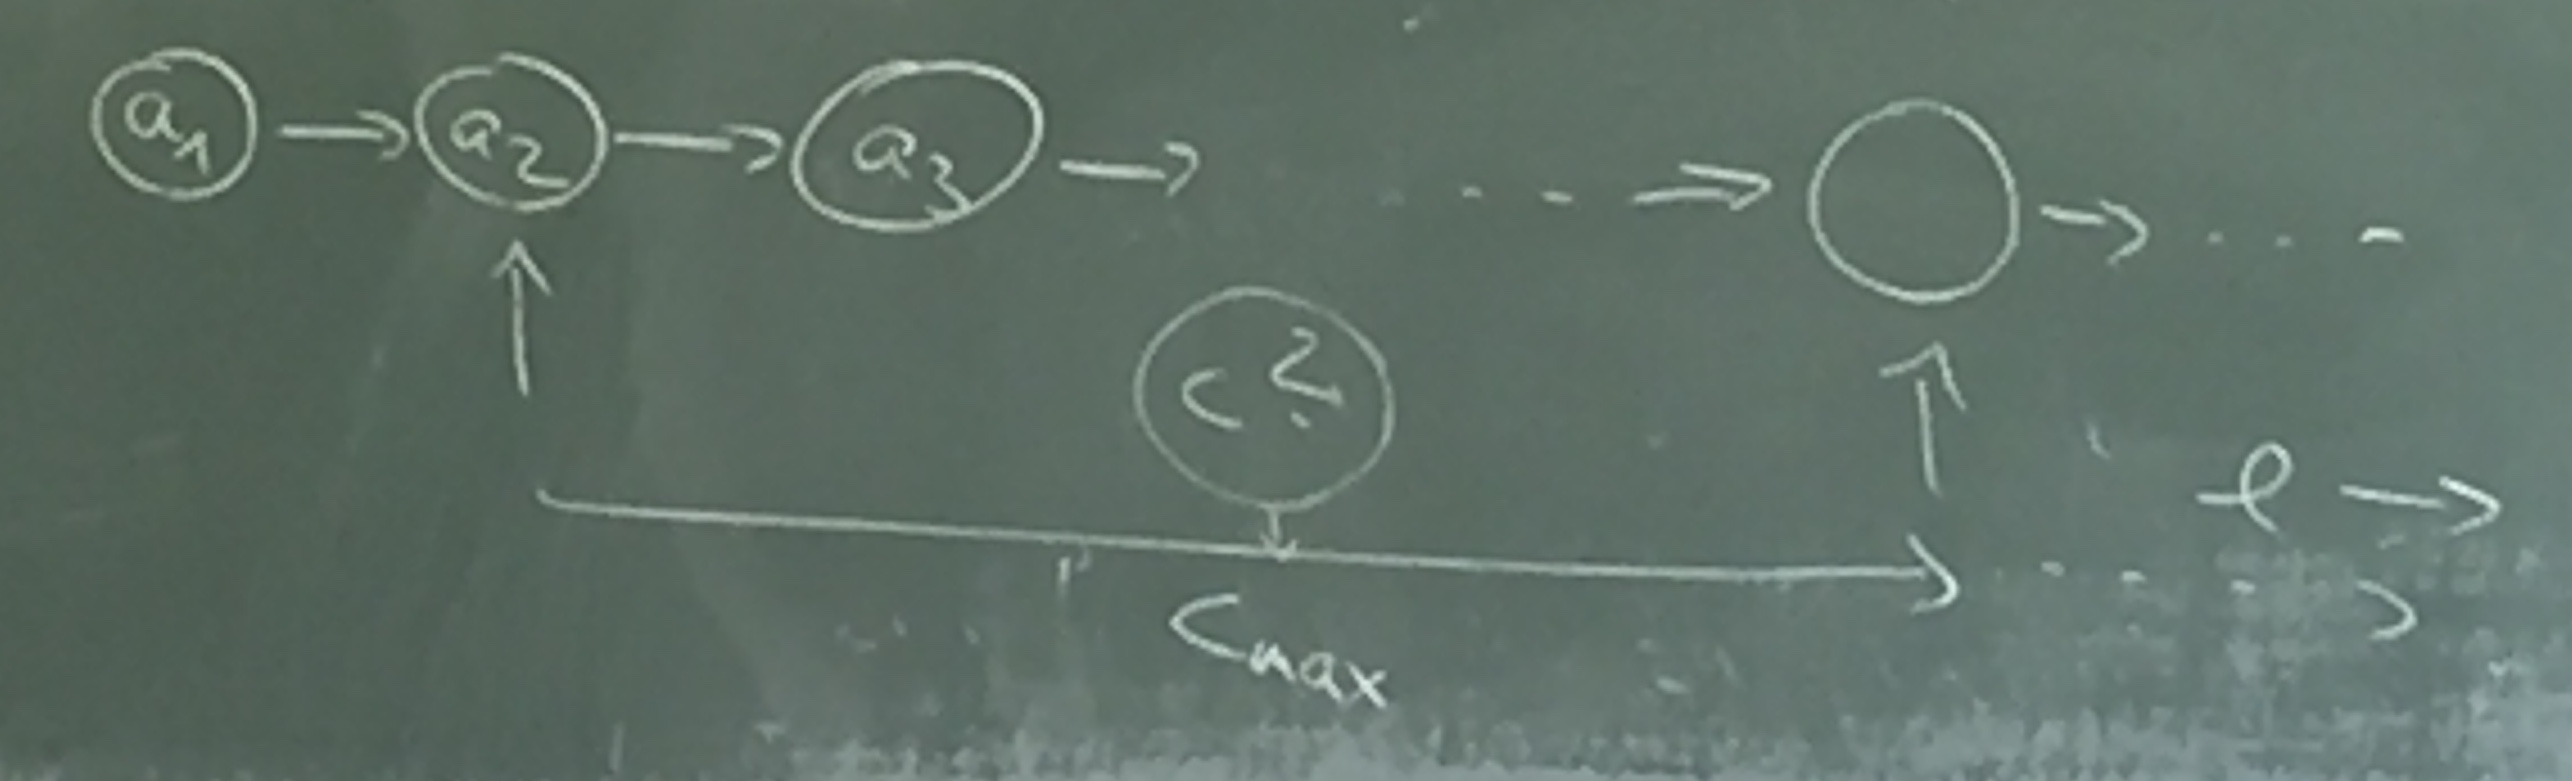
\includegraphics[width=0.7\linewidth]{img/img18}
\caption{}
\label{fig:img18}
\end{figure}

\subsubsection*{Lemma 2.1} 
Sei e ein beliebiger RA-Ausdruck, der zum Wertebereich $\{ a_1, a_2, a_3, \cdots \}$ passt und zu RT. Dann lässt sich $e(R_l)$ für ein genügend großes l darstellen als
\begin{align*}
&e(R_l) = \{ (X_1, \cdots, X_K) / \Psi(X_1, \cdots, X_K) \} \subseteq \{ a_1, \cdots, a_l \}^K
\end{align*}

mit $K \in \mathbb{N}$, $\Psi$ aussagenlogischer Ausdruck in disjunktiver Form, wobei atomare Ausdrücke nur Vergleichsausdrücke der oben genannten Form auftreten.

\paragraph*{Beweis:} (durch Induktion über den Aufbau von e)
\textbf{Annahme:} Abarbeitungsreihenfolge für e festgelegt, etwa durch vollständige Klammerung. Die Tiefe von e sei m. \\
\textbf{Induktionsanfang:} $n = 0 \leadsto $ Operand isr $R_l$ oder Teilmenge $\{ c_1, \cdots, c_m \} \subseteq \{ a_1, \cdots, a_l \}$
\begin{align*}
&R_l: \{ (X_1, X_2) | X_2 = X_1 \uparrow 1 \}\footnotemark \\
&\{c_1, \cdots c_n \} : \{ (x) | x = c_1 \vee x = c_2 \vee \cdots \vee x = c_m \}
\end{align*}
\footnotetext{Wegen $R_l = \{(a_1, a_2), (a_2, a_3), \cdots \}$}

\textbf{Induktionsannahme:} Lemma gilt für alle Anfragen mit Tiefe kleiner gleich m.
\textbf{Induktionsschluss:} 
\begin{align*}
& e = e_1 \cup e_2 \quad e = e_1 \backslash e_2 \quad e = e_1 \times e_2 \\
& \Psi_1() \wedge \lnot \Psi_2() \quad (b_1, \cdots, b_k, b'_1, \cdots, b'_{k'}) / \Psi_1() \wedge \Psi_2() \quad ()/\Psi() \wedge F()
\end{align*}

\textbf{Schwieriger:} Projektion, allgemein darstellbar als: \\
Permutationen + Projektionen mit Elimination der letzten Stelle. Wirkung von Permutationen klar (wir haben in $\Psi$ ja Variablen) $\Rightarrow$ interessant: $e = e_1[1, \cdots, K-1]$. \\
Sei $e \sim \{ (X_1, \cdots, X_K) | \Psi(X_1, \cdots, X_K) \} \leadsto e \sim \{(X_1, \cdots, X_{K-1}) | (\exists X_k) (\Psi(X_1, \cdots, X_k) \}$\footnote{Nicht gewünschte Form}

$\Psi = \Psi_1 \vee \cdots \vee \Psi_P$ nach Annahme, $\Psi_i$ konjunktiver Ausdruck \\
Damit $e \sim \bigcup^{\uparrow}_{i = 1} \{ (X_1, \cdots, X_{K - 1}) | (\exists X_K)(\Psi_i(X_1, \cdots, X_k)) \}$ \\
$\Rightarrow$ Betrachte nur noch \textit{konjunktive Ausdrücke} $\Psi$ ($\cup$ erledigt) \\

\paragraph{Fall 1:} Es gibt in $\Psi$ keine atomaren Ausdrücke der Form
$X_K = a_j, \quad X_K = X_i \uparrow c, \quad X_i = X_K \uparrow c$ mit K Index der letzen Komponente.
Sei $\Psi'$ die Konjunktion aller Atome von $\Psi$, die kein $X_K$ enthalten\footnote{Wirf Atome mit $X_K \neq \cdots$ raus} \\
Dann gilt
\begin{align*}
&* e \sim \{ (X_1, \cdots, X_{K - 1}) | \Psi'(X_1, \cdots, X_{K - 1} \} 
\end{align*}

Beispiel

\begin{align*}
& e_1 \sim \{ (X_1, X_2, X_3) | X_2 = X_1 \uparrow 1 \wedge X_2 \neq X_3 \uparrow 0 \wedge X_3 \neq X_1 \uparrow 2 \} \\
& e = e_1[1,2] \leadsto e \sim \{ (X_1, X_2) | X_2 = X_1 \uparrow 1 \}
\end{align*}

Begründung für * 

\underline{Annahme}: $(b_1, \cdots, b_{K-1}$ erfüllt $\Psi'$, für genügend großes l kann für $X_k$ ein $a_m$ gewählt werden $(\exists)$, so dass alle Atome $X_k \neq a_j, \quad X_k \neq X_i \uparrow c, X_i \neq X_K \uparrow c$ erfüllt sind. Dan erfüllt $(b_1, \cdots, b_{K - 1})$ auch $(\exists X_K)(\Psi(X_1, \cdots, X_K)$. \\
Umgekehrt: $(b_1, \cdots, b_{K - 1})$ erfülle $(\exists X_K)(\Psi(X_1, \cdots, X_K)$. Dann erfüllt $(b_1, \cdots, b_{K - 1})$ insbesndere alle Atome, die $X_K$ nicht enthalten.

\paragraph{Fall 2:} Es gebe in $\Psi$ \underline{ein} Atome der Form $X_K = a_j, \quad X_K = X_i \uparrow c \text{ oder } X_i = X_K \uparrow c$ sei es mit $\upxi$ benannt. \\
Falls mehrere vorhanden: wähle ein aus, ersetze $X_K$ in allen anderen Vorkommen durch $a_j, \quad X_i \uparrow c \text{ bzw } X_i \uparrow c' (c' = -c)$. Lasse $\upxi$ weg. \\
Mögliche Folge dieser Einsetzung im Ausdruck $\Psi$:
\begin{itemize}
\item atomare Ausdrücke, die direkt zu wahr oder falsch ausgewertet werden können: Bei wahr weglassen, bei falsch $e \sim \{ X_1, \cdots, X_{K - 1} \} = \emptyset$
\item nicht zulässige Ausdrücke: $\leadsto$ geeignet umformen: \\
\begin{align*}
&a_j \uparrow c \rightarrow a_{j+c} \quad a_j = X_k \uparrow c \rightarrow X_K = a_{j - c} \\
&X_i \uparrow c = a_i \rightarrow X_i = a_{j - c} \\
& X_i \uparrow c \uparrow c' \rightarrow X_i \uparrow c'', c'' = c + c' \\
& X_i \uparrow c = X_k \uparrow c' \Rightarrow X_i = X_k \uparrow c'' mit c'' = c' - c 
\end{align*}
Analog bei $\neq$
Falls nicht ``falsch'' als Ergebnis enthalten werden kann gilt $e \sim \{ (X_1, \cdots, X_{K - 1}) | \Psi'(X_1, \cdots, X_{K - 1} \}$, wobei $\Psi'$ aus $\Psi$ wie folgt erhalten wird:
\begin{itemize}
\item Ersetze und forme um wie oben angegeben
\item Ausgewähltes Atom $\upxi$ hat die Form $X_K = X_i \uparrow c, c \ge 0 \text{ oder } X_i = X_k \uparrow c, c \le 0$. Füge Atome $X_i \neq a_j$ für $l-c < j \le j$ hinzu. \footnote{Damit $X_K$ nicht aus dem Wertebereich führt}
\item Ausgewähltes Atom $\upxi$ hat die Form $X_K = X_i \uparrow c, c < 0, \text{ oder } X_i = X_K \uparrow c, c > 0 \rightarrow$ Füge Atome $x_i \neq a_j$ für $1 \le j \le c$ hinzu. Damit: Zu jeder Belegung $a_i$ von $x_i$ wird ein $a_j$ mit $a_ = a_{i + c}$ gefunden.
\paragraph{Beispiel:} $(\exists x_3)(\cdots, x_3 = x_2 \uparrow 2 \cdots) \leadsto (\cdots \wedge X_2 \neq a_4 \wedge x_2 \neq a_5 \wedge \cdots$
\end{itemize}
\end{itemize}

\subsubsection*{Beweis von Satz 2.3}
Betrachte Wertebereich $\{ a_1, a_2, a_3, \cdots \}$ und passende RA-Ausdrücke mit RT i Teilmenge des Wertebereichs als Operanden. \\
\paragraph{Annahme:} Es gibt e mit $e(RT) = RT^+$ \\
$\leadsto$ Für jede Relation $R_l$ filt $e(R_l) = R_l^+$ \\
$\leadsto$ (Lemma 2.1) $e \sim \{ (X_1, X_2) | \Psi(X_1, X_2) \}$

\paragraph{1. Fall:}
Jeder konjunktive Ausdruck von $\Psi$ hat ein Atom der Form 
\begin{align*}
x_i = a_j, \quad x_2 = a_j, \quad x_1 = x_2 \uparrow c, \quad x_2 = x_1 \uparrow c
\end{align*}
Bei genügnd großen l gibt es ein Intervall [$q_1, q_2$], in dem Indizes m und m+d liegen, so dass $(a_m, a_{m+d}$ keinen konjunktiven Ausdruck von $\Psi$ erfüllt, aber in $R_l^+$ enthalten ist!
Wähle m größer als jedes vorkommende j (es gibt ein größtes festes ``j'' in $\Psi$) bzw d größer als jedes ``c'' $\Rightarrow$ kein konjunktiver Term erfüllt $(a_m, a_{m-d})$.

\paragraph{2. Fall:}
Es gibt einen konjunktiven Ausdruck in $\Psi$, dessen Atome alle von der Form
\begin{align*}
x_i \neq a_j, \quad x_2 \neq a_j, \quad x_1 \neq x_2 \uparrow c, \quad x_2 \neq x_1 \uparrow c
\end{align*}

Falls l genügend groß, gibt es ein Paar $(a_{m+d}, a_m)$, das den Ausdruck erfüllt, aber nicht in $R_l^+$ liegt. Das führt zum Wiederspruch.

Einfache Erweiterung, um Hüllenberechnung zu ermöglichen: \\
Erlaubte Gleichungen (vgl. Datalog-Übersetzung) der Form \\
\begin{align*}
&RT = f(RT) \\
&(RT, \{ A_1, \cdots, A_k \}), \{ A_1, \cdots, A_k \} \subseteq \alpha_0 \\
& RT \in \{ RT_1, \cdots, RT_m \}
\end{align*}

\paragraph{$f(RT):$} RA-Ausdruck, der bis auf RT zu $\sigma$ passt, und der nicht die Differenz enthält ($\leadsto$ monoton).
\paragraph{Beispiel}: Sei $(S, \{A, B \})$ ein binärer Relationstyp und o die Komposition von Relationen mit Darstellung $R_1 o R_2 = (R_1 \bowtie R_2)[1,4]$.

\paragraph{Hülle von S:} kleinster Fixpunkt von $R = R o S \cup S$. \\
Berechnung (Fixpunktsatz): $f^{m_0}(\emptyset) = \bigcup^{\infty}_{i = 1} S o \cdots o S\footnote{i-Mal}$, $m_0$ Zahl mit $f^{m_0}(\emptyset) = f^{m_0 + 1}(\emptyset)$

\paragraph{Frage:} Wann soll eine Anfragesprache als vollständig bezeichnet werden?

Oben: $q | \Upxi_\delta \rightarrow R^\infty_\beta \leadsto$ 

\begin{itemize}
\item getypt (vollständige Signatur), mögliche Verallgemeinerung: $q | \Upxi_\delta \rightarrow \bigcup_{B \subseteq \alpha} R^\infty_\beta$
\item q Fukntion $\leadsto$ nicht möglich: ``Gib Daten für einen beliebigen Angestellten.''
\end{itemize}

Bsp:

\begin{lstlisting}[language=SQL]
select * 
from ANG a, (select count(*) as N from ANG) as N of ANG
where cast((rand() * 1000) / N of ANG N) as integer
= (select rank() over (order by a.Name) as Rank_number
from ANG a)
\end{lstlisting}

\subsubsection*{Forderungen}
\begin{enumerate}
\item q berechenbar (partiell rekursiv) $\leadsto$ $R_\beta$ statt $R^\infty_\beta$
\item q generisch (isomorphietreu)
\end{enumerate}

\paragraph{zu 2.} Sei mit Dom die Menge aller Wertebereichelemente bezeichnet. Sei $C \subseteq Dom$, C endlich, sei $z \in \Upxi_\delta$ \\
q heißt C-generisch, falls für jede Permutation $\rho$ auf Dom mit $\rho(x) = x$ für alle $x \in C$ folgendes Diagramm kommutiert:
\begin{figure}[h!]
\centering
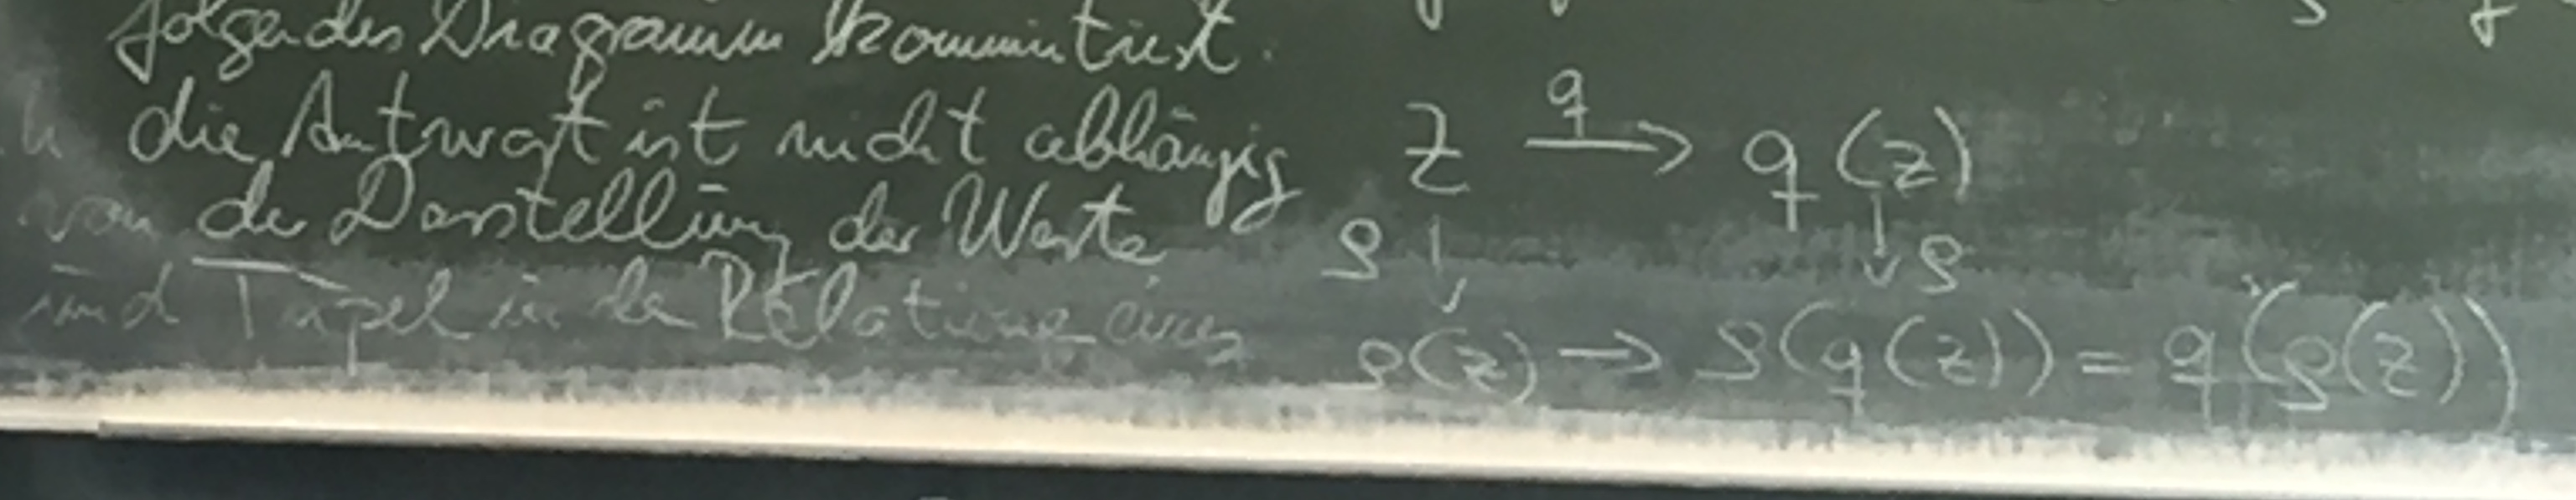
\includegraphics[width=0.7\linewidth]{img/img19}
\caption{}
\label{fig:img19}
\end{figure}

Falls $C = \emptyset$ heißt q generisch. \\
Bedeutung von C: enthält die in q verwendeten Konstanten(symbole). $C = \emptyset$ immer möglich: Verwende ``konstante'' Relationen als Operanden ($\{A : c \}$) $\leadsto$ keine Konstanten(symbole) in Anfrage notwendig.

\begin{figure}[h!]
\centering
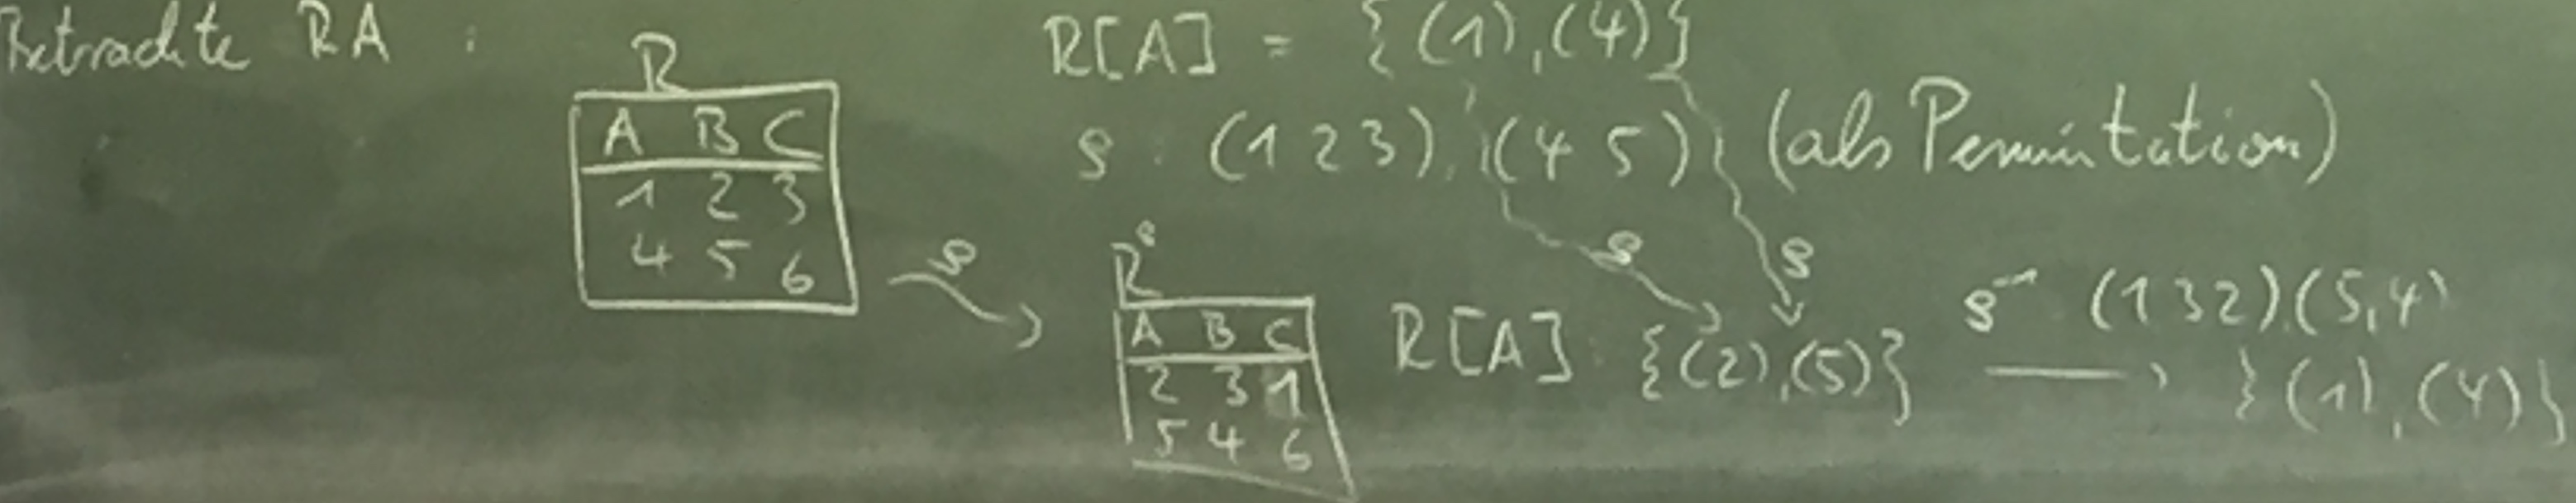
\includegraphics[width=0.7\linewidth]{img/img20}
\caption{}
\label{fig:img20}
\end{figure}

\subsection*{Definition: Vollständigkeit einer Anfragesprache}

Eine Anfragesprache $(L_0, \mu)$ zu einem DB-Schema $\sigma$ heißt vollständig, wenn gilt: 
\begin{enumerate}
\item Für jeden Ausdruck $e \in L_\sigma$ ist $\mu(e)$ berechenbar und generisch
\item Für jede berechenbare und generische Anfrage q an $\sigma$ gibt es einen Ausdruck $e \in L_\sigma$ mit $\mu(e) = q$.
\end{enumerate}


\subsection*{Definition: Abgeschlossenheit einer Anfragesprache}

Eine allgemeine Anfragesprache L mit Interpretationsvorschrift $\mu$ heißt abgeschlossen, wenn sie zu jedem Datenbank-Schema $\sigma$ eine vollständige Anfragesprache $(L_\sigma, \mu)$ enthält.
Offensichtlich: 
\begin{itemize}
\item Alle RA-Anfragen sind berechenbar und generisch
\item Die RA ist nicht abgeschlossen (s. Satz 2.3)
\end{itemize}

\paragraph{Frage:} Wie RA zu vollständiger Spache erweitern? Problem? Effizient? (Weitere Diskussion später) \\
Oben: Fixpunktoperator. Reicht allein nicht. \\
Bsp. PERSON(Vname, Geschlecht) \\
Anfrage: ``Ist die Anzahl weiblicher Personen gerade?''

\subsubsection{Vorschlag für abgeschlossene Sprache QL}

Programmiersprache (Zuweisungen, while-Konstrukt, Hintereinanderausführung von Anweisungen) mit eingeschränkter Menge von Datenbankoperationen.

\begin{itemize}
\item Gleichheit
\item Komplement
\item Durchschnitt
\item Test auf Leerheit
\item vereinfachte Versionen der Projektion und des kartesischen Produkts $\leadsto$ Simulation beliebiger Turingmaschinen
\end{itemize}

\paragraph{Vereinfachung:} \textbf{ein} Wertebereich Dom, Relationen $\subset Dom^i$, i Stelligkeit der Relation (rank(R))

\subsection{QL-Syntax:} Seien $x_1, x_2, \cdots$ Variablen, $r_1, r_2, \cdots$ Relationen \\

\paragraph{Definition: QL-Terme}
Die Menge der \textbf{QL-Terme} ist induktiv definiert:
\begin{enumerate}
\item E (Gleichheit) ist ein Term, $r_i, x_i$ sind Terme
\item Falls e, e' Terme sind, dann $(e \cap e'), (\lnot e), (e \downarrow), (e \uparrow) \text{ und } e\circlearrowright$
\end{enumerate}


\paragraph{Definition: QL-Programme}
Die Menge der \textbf{QL-Programme} ist induktiv definiert durch

\begin{enumerate}
\item $x_i := e$ ist ein Programm für einen Term $e$ und $i \ge 1$
\item Für Programme $P,P'$ sind $(P; P')$ und \texttt{while } $x_i$ \texttt{do P} Programme. Es gelten die üblichen Klammereinsparungsregeln
\end{enumerate}

\paragraph{Beispiel}

\begin{align*}
&x_2 := x_1, \quad x_3 := E \downarrow\downarrow\downarrow; \\
& while x_2 do (P; x_2 := e; x_3 := E); \\
& while x_3 do (P'; x_3 := E);
\end{align*}


\paragraph{QL-Semantik}

Seien $\sigma = \{ (RT_1, s_1), \cdots, (RT_m, s_m) \},\quad s_i \in \mathbb{N}, \quad z \in \xi_\sigma$.
\begin{itemize}
\item $R^\emptyset_S:$ leere Relation der Stelligkeit s
\item $R_S:$ Menge der Relationen mit Stelligkeit
\item $R_{-1} = \{ R^\emptyset_0 \}$
\end{itemize}

$\leadsto E \in R_2$  mit $E = \{ (d,d) | d \in Dom \}$ \\

\begin{itemize}
\item $r_i = \begin{cases} z(RT_i) \text{falls } i \le m \\ R^\emptyset_0, \text{sonst} \end{cases}$
\item ``$\cap$'' entspricht Durchschnitt, falls beide Argumente gleiche Stelligkeit haben, sonst $R^\emptyset_0$
\item ``$\lnot$'': $R_S \rightarrow R_S$: $\lnot e =_{def} Dom^s - e$
\item ``$\downarrow$'' $R_S \rightarrow R_{s-1}$: $e\downarrow =_{def} \{ (d_2, \cdots, d_s) | (d_1, \cdots, d_s) \in e \}$
\item ``$\uparrow$' $R_S \rightarrow R_{s+1}$: $e\uparrow =_{def} \{ (d_2, \cdots, d_s, d) | (d_1, \cdots, d_s) \in e, d \in Dom \}$
\item ``$\circlearrowright$'' $R_S \rightarrow R_S$: $e\circlearrowright =_{def} \{ (d_1, \cdots, d_{s-2}, d_s, d_{s-1}) | (d_1, \cdots, d_s) \in e \}$
\end{itemize}

\paragraph{Bemerkung}
\begin{align*}
&\lnot (Dom^S) = R^\emptyset_S \quad e\downarrow = \{ () \} \text{falls Stelligkeit von e gleich 1 und } e \neq R^\emptyset_1 \\
&\{()\}\uparrow = E\downarrow = Dom \\
&E\downarrow = \{(d)\}\\
&E\downarrow\downarrow = \{()\}\\
& E\downarrow\downarrow\downarrow = \emptyset?
\end{align*}


\begin{itemize}
	\item Alle Variablen werden mit $R^\emptyset_0$ initialisiert
	\item Test von $x_i$ in while-Anweisung ist wahr $\diamondsuit_{def} x_i$ ist nicht leer
\end{itemize}


\subsubsection*{Satz 2.4} 
QL ist abgeschlossen

\paragraph*{Beweisidee}

Zeige zunächst, dass einige übliche Operationen auf Relationen ausdrückbar sind, etwa zählen:

\begin{align*}
& 0: E \downarrow\downarrow (= \{()\})
\end{align*}

Ebenso ausrückbar:
\begin{align*}
&e_1 \times e_2 \text{(kartesisches Produkt)} \\
&e[s_1, \cdots, s_p] \text{(allgemeine Projektion)} \\
&e\uparrow \text{(Projeziere links hinein} d,d_1,\cdots,d_s)
\end{align*}

Sei $e$ Darstellung von $i \quad i+1 : e\uparrow \quad i-1: e\downarrow$ \\ Test von e auf 0: Teste $e\downarrow$ auf Leerheit mit if + while $\leadsto$ s.o.

\paragraph{Transitive Hülle} 
$x_1 := E; \quad x_2 := r_1; \quad x_3 := \lnot (\lnot E \cap \lnot x_2); \quad x_4 := \lnot E \cap x_2;$ \\
while $x_4$ nicht leer do ($x_1 := x_3; x_3 := x_3 \cup (((x_3 \times x_2) \cap \uparrow E \uparrow)_{[1,4]}); x_4 = \lnot x_1 \cap x_3$)

\paragraph{Einfach:} QL-Programme sind partiell rekursiv und generisch. Schwieriger: Jede berechenbare und generische Anfrage lässt sich als QL-Programm schreiben.

Andere Idee für Erweiterung: Erweitere TRC geeignet um arithmetische Operationen für $\mathbb{N}$, (Gödel: In einer Sprache der Arithmetik erster Stufe lassen sich alle rekursiven Funktionen ausdrücken)

\subsection*{Tupelorientierter Relationenkalkül}
PL1-Logike $\rightarrow$ getypter Kalkül (DB-Schema beachten)


\begin{figure}[h!]
\centering
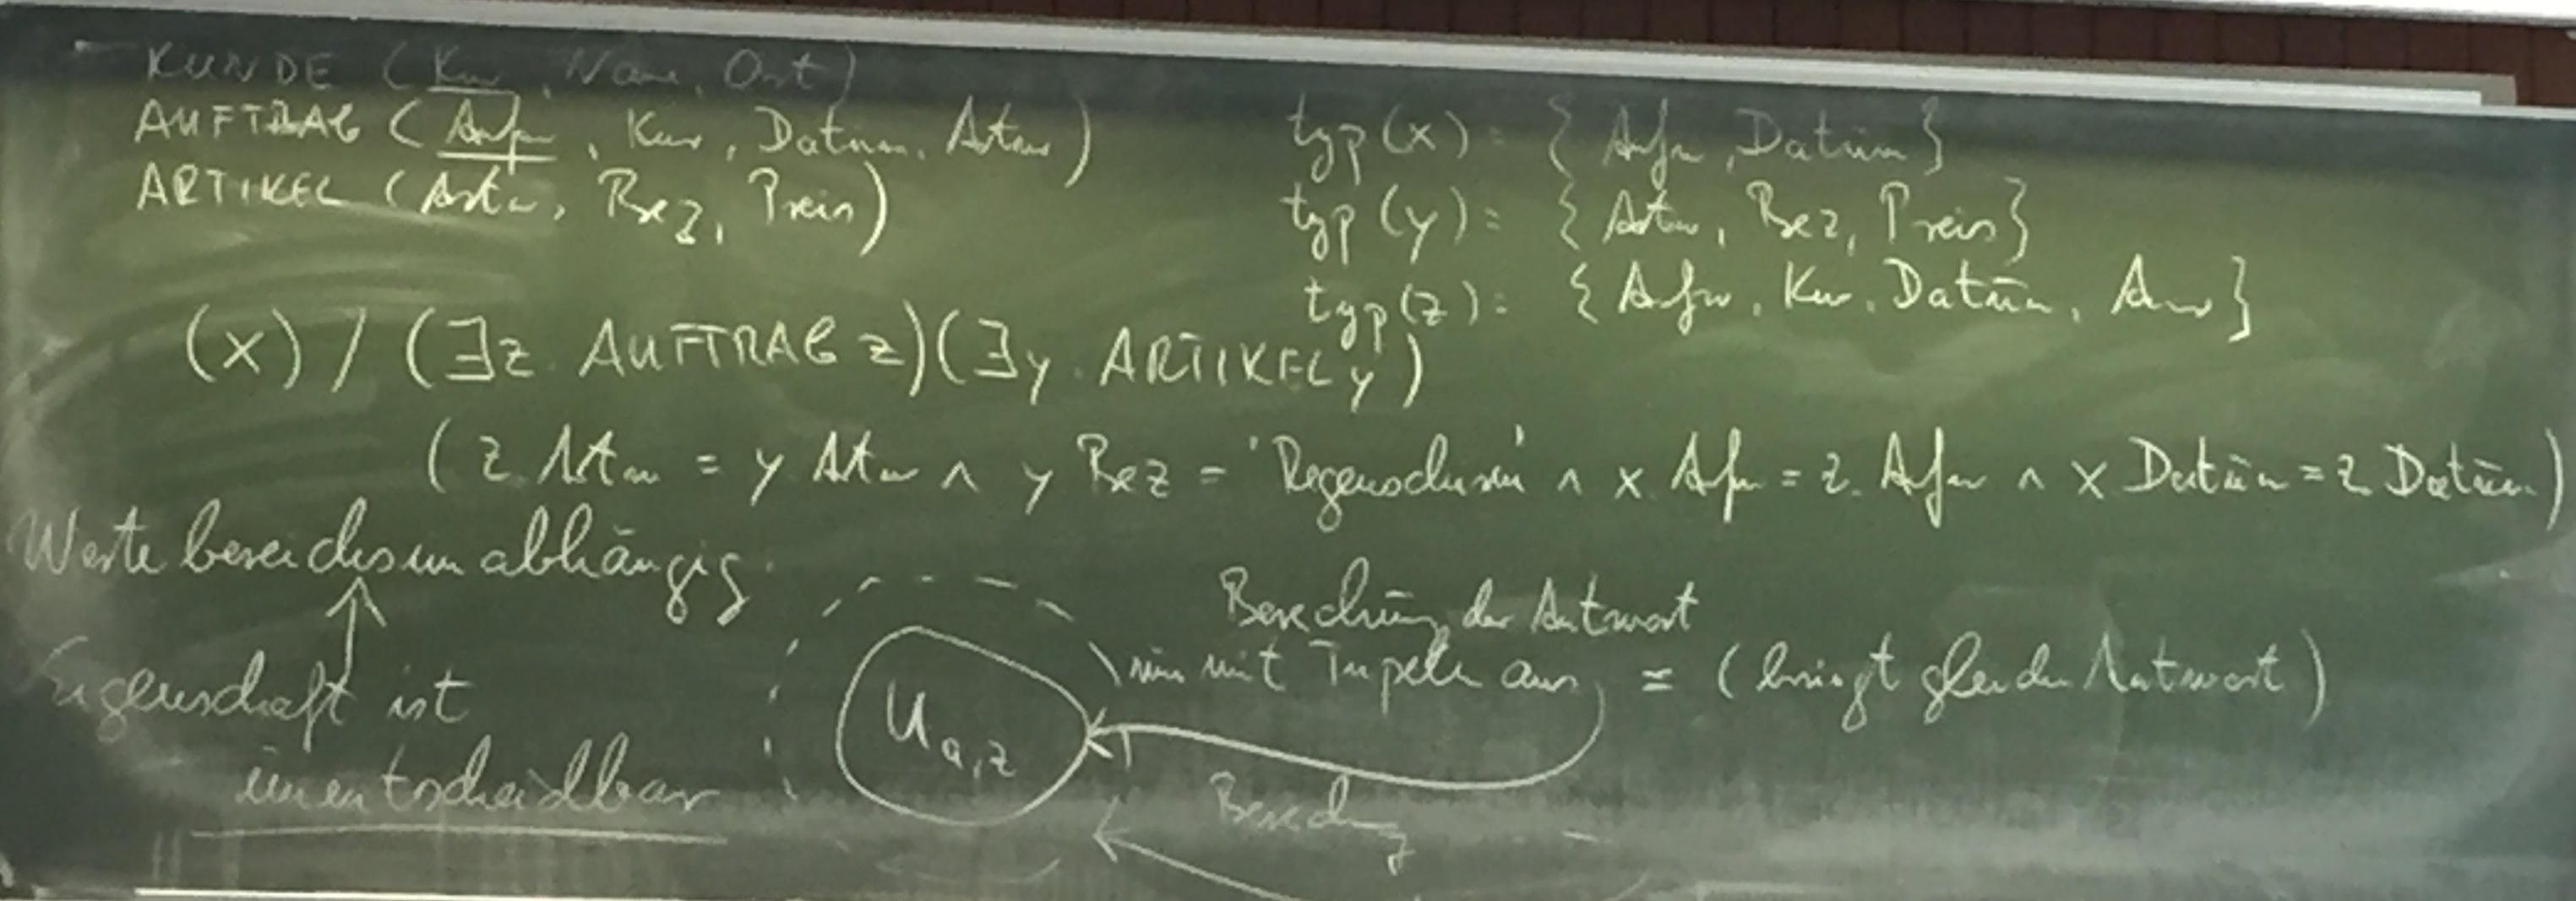
\includegraphics[width=0.7\linewidth]{img/img22}
\caption{}
\label{fig:img22}
\end{figure}

\begin{figure}[h!]
\centering
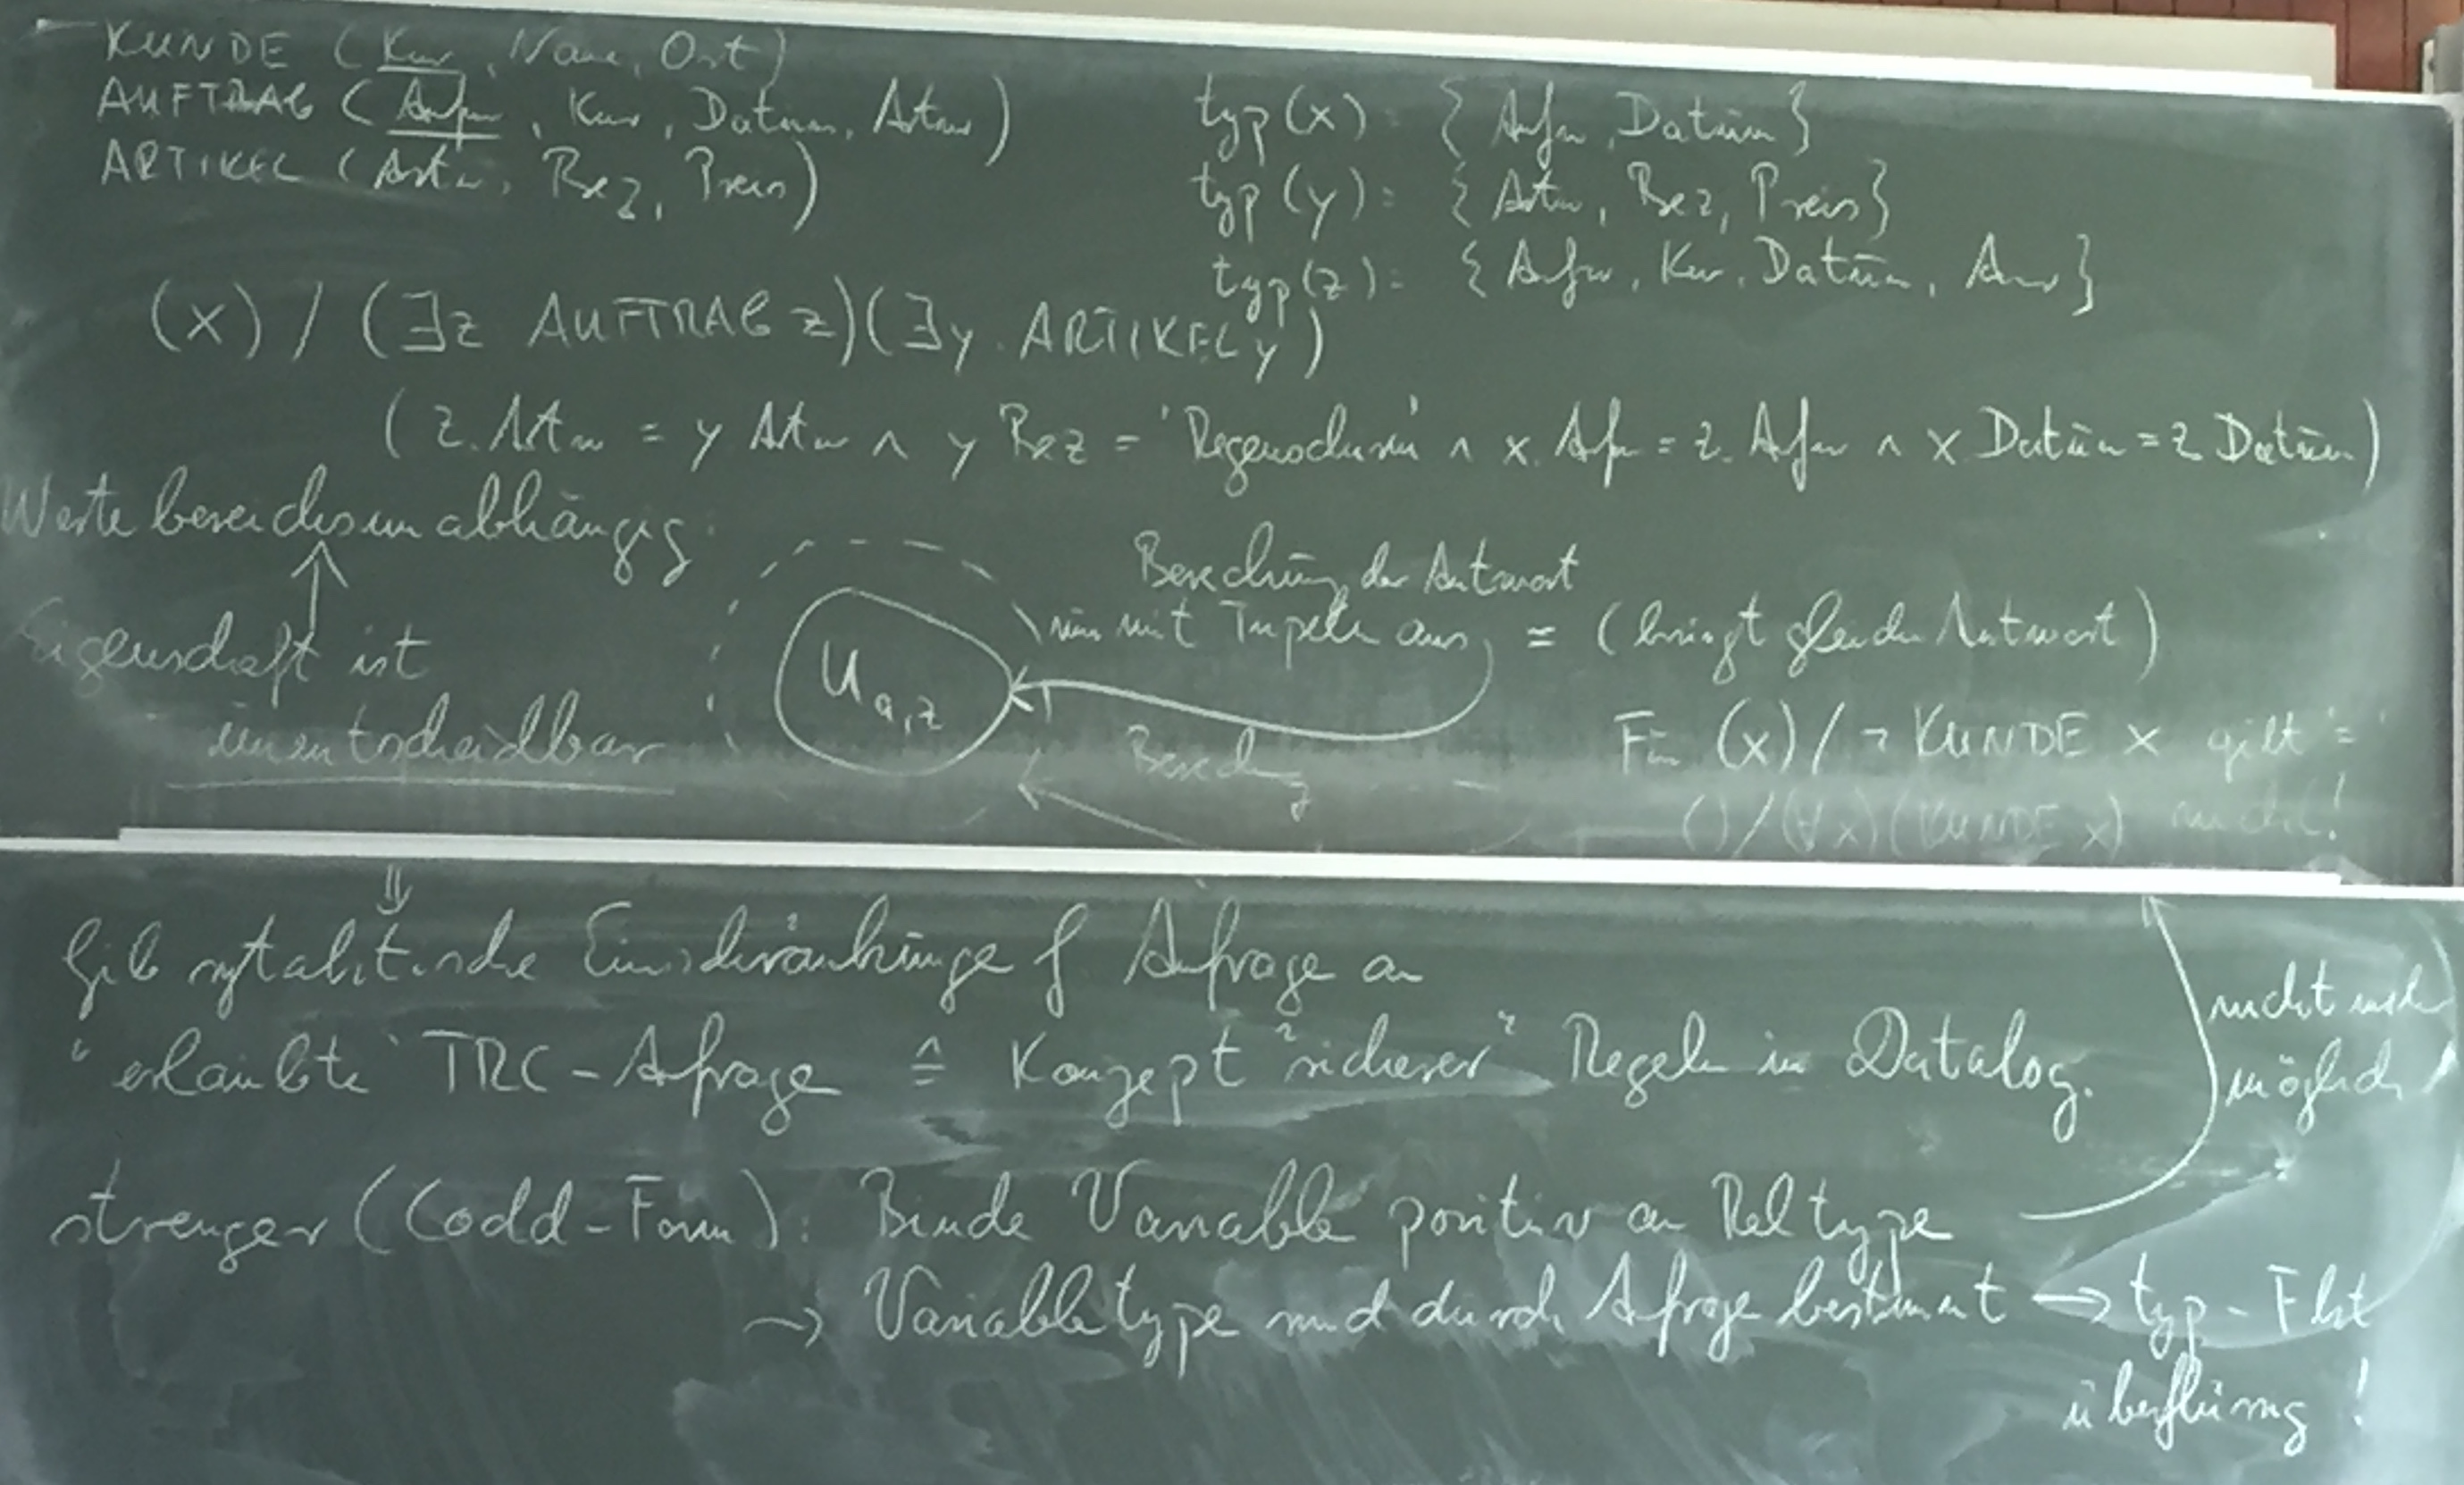
\includegraphics[width=0.7\linewidth]{img/img23}
\caption{}
\label{fig:img23}
\end{figure}

\paragraph{Beispiel:} 
\begin{align*}
&typ(x) = \{A,C\}, \quad typ(y) = \{B,C\}, \quad typ(z) = \{A,B\} \\
& (x,y B) / R.x \wedge S.y \wedge (\forall z: Tz)(z.A = x.A \wedge z.B > y.B) \\
& R.x \leadsto R[A \rightarrow x\_A, C \rightarrow x\_C] \\
& S.y \leadsto S[B \rightarrow y\_B, C \rightarrow y\_C]\footnotemark \\
& (\forall z: T.z)(\cdots) \leadsto ((( R \backslash R)[A][A \rightarrow z.A][Kompl]  \\
&\times \cdots \times (R \backslash R)[A][A \rightarrow x\_A][kompl] \times \cdots \times x\_c \cdots)[z.A = x.A]) \\
&\cap \cdots \text{ analog } \cdots \times (R \backslash R)[A][A \rightarrow x\_A][kompl] \times \cdots \times x\_c
\end{align*}

\footnotetext{$\{ \emptyset \}$ entspricht nicht-leere Relation über leerer Attributmenge, d.h. enthält das total undefinierte Tupel}

\section*{Komplexität von Anfragesprachen}

Zur Erinnerung: Komplexitätsklassen

\paragraph{Zeit}
\begin{itemize}
	\item DTIME(n) $\le$ DTIME($n^2$) $\le$ P = PTIME = $\bigcup_{k \in \mathbb{N}} DTIME(n^K)$
	\item NTIME(n) $\le$ NTIME($n^2$) $\le$ NP = NPTIME = $\bigcup_{k \in \mathbb{N}} NTIME(n^K)$
	\item EXPTIME = $\bigcup_{k \in \mathbb{N}} DTIME(n^{P(K)})$
\end{itemize}

\paragraph{Platz}
\begin{itemize}
	\item LOGSPACE = DTAPE(log n)\footnote{mit Speicheplatz O(S(n))}
\end{itemize}

$DTAPE(n) \subseteq DTAPE(n^2) \cdots DPSPACE = \bigcup_{d \in \mathbb{N}} DTAPE(n^K)$ \\
$NTAPE(n) \subseteq NTAPE(n^2) \cdots NPSPACE = \bigcup_{d \in \mathbb{N}} NTAPE(n^K)$ 

\subsection*{Inklusionssatz}

\begin{align*}
LOGSPACE \subseteq^? NLOGSPACE \subseteq^? P &\subseteq^? NP  \\
\subseteq^? PSPACE \subseteq NPSPACE \subseteq EXPTIME &\subseteq REK
\end{align*}

\begin{itemize}
\item P $\leadsto$ explizite Anfrage
\item PSPACE $\leadsto$ while Anfrage
\end{itemize}

\paragraph{Frage}
Was ist die Problemgröße bei Anfragen an Datenbanken? \\
2 Möglichkeiten:
\begin{itemize}
	\item Länge der Anfrage (DB fest) $\leadsto$ ''Anfragenkomplexität``
	\item Größe der DB (q fest) $\leadsto$ ''Datenkomplexität``
\end{itemize}

\paragraph{Erkennungsproblem für Anfragen} Gegeben ein DB-Zustand  $z$ zu einem DB-Schema $\sigma$, Anfrage $q | \phi_\sigma \rightarrow R_\beta$ und Tupel t über $\beta. \leadsto$ Stelle fest, ob $t \in q(z)$.

\begin{align*}
&\{ code_E(z) \# code_E(t) | t \in q(z), E \text{ Aufzählung von} DOM_{q,z} \} \\
&E =  \{ d_1, d_2, \cdots \}
\end{align*}


\subsection*{Definition: Datenkomplexität einer Anfrage}
Die Datenkomplexität\footnote{kurz: Komplexität} einer Anfrage q ist die Komplexität ihres Erkennungsproblems. Größe des Ergebnisses (der Antwort) ist nicht erfasst. Falls gewünscht \textbf{|Antwortkomplexität}: $\{ code_E(z) + code_e(q(z))  | \cdots \}$ Komplexität der Konstruktion des Ergebnisses erfasst. \\
Unterschied nicht wesentlich bei Komplexitätsklassen, die bzgl. Polynomialfaktor unempfindlich sind (ab ''P`` aufwärts) \\

\textbf{Aber} Mit Antwortkomplexität keine Unterscheidung zwischen leichten und schwierigen Anfragen, die große Ergebnisse haben möglich

\paragraph{Beispiel}

\begin{align*}
&\sigma = \{ (G, \{ V_1, V_2 \}) \} (Graph) \\
& 1) kart(G) = G[V_1] \times G[V_2] \\
&2) pfade(G) = \{ (x,y) | \text{es gibt einen Pfad zwischen x und y} \} \\
&3) ident(G) = G
\end{align*}

Betrachte Zeitkomplexität: 
\begin{itemize}
\item 1) $\leftrightarrow$ 2) Antwortkomplexität: $O(n^2)$ bei 1) und 2) \\
Datenkomplexität: 1) O(n), 2) O($n^2$)
\item 1) $\leftrightarrow$ 3): Antwortkomplexität 1) $O(n^2)$, 3) O(n) \\
Datenkomplexität: O(n) 1) + 3)
\end{itemize}


\paragraph{Betrachte $\bowtie$} 
Datenkomplexität: O(n log n), Antwortkomplexität: $O(n^2)$ \\

Im Folgenden: Komplexität entspricht Datenkomplexität. Zunächst: L $\rightleftarrows$ Komplexitätsklasse

\paragraph{Problem:} Falls auf Wertebereichen keine Ordnung angenommen:
\begin{itemize}
	\item Für PRTIME und Klassen darunter sind keine Sprachen bekannt, die genau einer Komplexitätsklasse entsprechen
	\item Anderer Zusammenhang von Interesse: Bezug auf vollständige Probleme einer Klasse
\end{itemize}

\paragraph{Definition: Vollständiges Problem:} schweres Problem (Problem lösen entspricht Menge entscheiden).
\paragraph{Definition: hartes Problem} Ein Problem heißt hart für eine Komplexitätsklasse K unter einem Reduktionstyp, falls jedes Problem in K mit einer Reduktion des Typs auf p reduziert werden kann. Falls p in K: p ist K-vollständig
\paragraph{Definition: Vollständigkeit bezüglich einer Komplexitätsklasse K} Eine Anfragesprache $L_\sigma$ zu einem DBSchema $\sigma$ ist vollständig bezüglich einer Komplexitätsklasse, falls gilt: 
Sei $Q_\sigma K$ die Menge aller Anfragen an $\sigma$ mit Komplexität K:
\begin{enumerate}
	\item $\{ \mu(e) | e \in L_\sigma \} \subseteq Q_\sigma K$
	\item $(\exists e \in L_\sigma)$(das Erkennungsproblem für e ist vollständig bezüglich K)
\end{enumerate}

L heißt vollständig bezüglich K, falls $L_\sigma$ für jedes $\sigma$ vollständig ist bezüglich K.
Wichtig in diesem Zusammenhang: Komplexität der Reduktion. \\

z.B. Vollständigkeit bei logarithmischen Platz bezüglich K bedeutet: Jede Anfrage kann mit logarithmischen Platzaufwand auf die vollständige Anfrage reduziert werden. Reduktion muss nicht in L ausdrückbar sein. Es kann einfache Anfragen in QK geben, die nicht in L ausdrückbar snid (obwohl einige vollständige Anfrage in QK in L ausdrückbar sind)

DB Menge undiffernzierter Elemente generisch $\leadsto$ einheitliche Behandlung in Anfrage. Wie ist ``erstes Element'' spezifiziert?

\subsection*{Turingmaschine (TM)}

Kodiert die Eingabe auf Band (``Hinschreiben'') liefert zusätzliche Information, die Lösung trivial macht (erstes Element steht links) (lineare Zeit) $\leadsto$ andere ``Rechengeräte'' erforderlich (keine Ordnung auf Band) $\leadsto$ Forschung ``generisch'' kann Aufgaben schwierig machen.

\subsubsection*{PSPACE - vollständige Probleme}: 
\begin{itemize}
\item QSAT $\Phi (x_1, \cdots, x_n)$ in konjunktiver Normalform: $(\exists x_1)(\forall x_2)(\exists x_3) \cdots : \Phi(x_1, \cdots, x_n)$ ist wahr?
\item GO
\item GEOGRAPHY (einzigartige Stadtnamenfolge mit letzter Buchstabe gleich erster Buchstabe des nächsten)
\end{itemize}

\subsubsection*{Komplexität von Kalkülanfragen (RA)}

\paragraph*{Annahme:} TM hat lesebeschränktes Eingabeband und Arbeitsband, Kodierung des DB-Zustands und der Anfrage auf Eingabeband sonst bedingt Kodierung des Zustandes, dass keine Komplexität unter ``linear'' möglich ist.

\paragraph{Beispiel für Kodierung $code_E$}
Nimm alle Elemente $U \subseteq DOM$ als durch Aufzählung E gegeben an: $E = \{c_1, c_2, \cdots \} $\\
$code_E | c_i \rightarrow \text{Binärdarstellung von i} \leadsto |code_E(c_i)| \le \lceil log(i) \rceil $ für jedes i

\paragraph{Kodierung}
\begin{itemize}
	\item Tupel: $t = (a_1, \cdots a_k) \leadsto^{code_e(t)} [code_E(a_1)\#code_E(a_2)\#\cdots\# code_E(a_k)$
	\item Relation: $R_i \leadsto^{code_e(R_i)} R_i code_E(t_1) \cdots code_E(t_n) \text{in durch } code_E$ gegebener lexikographischer Ordnung
	\item Zustand $z \leadsto^{code_E(z)} code_E(z(R_1))) \cdots code_E(z(R_m)))$
\end{itemize}

\begin{figure}[h!]
\centering
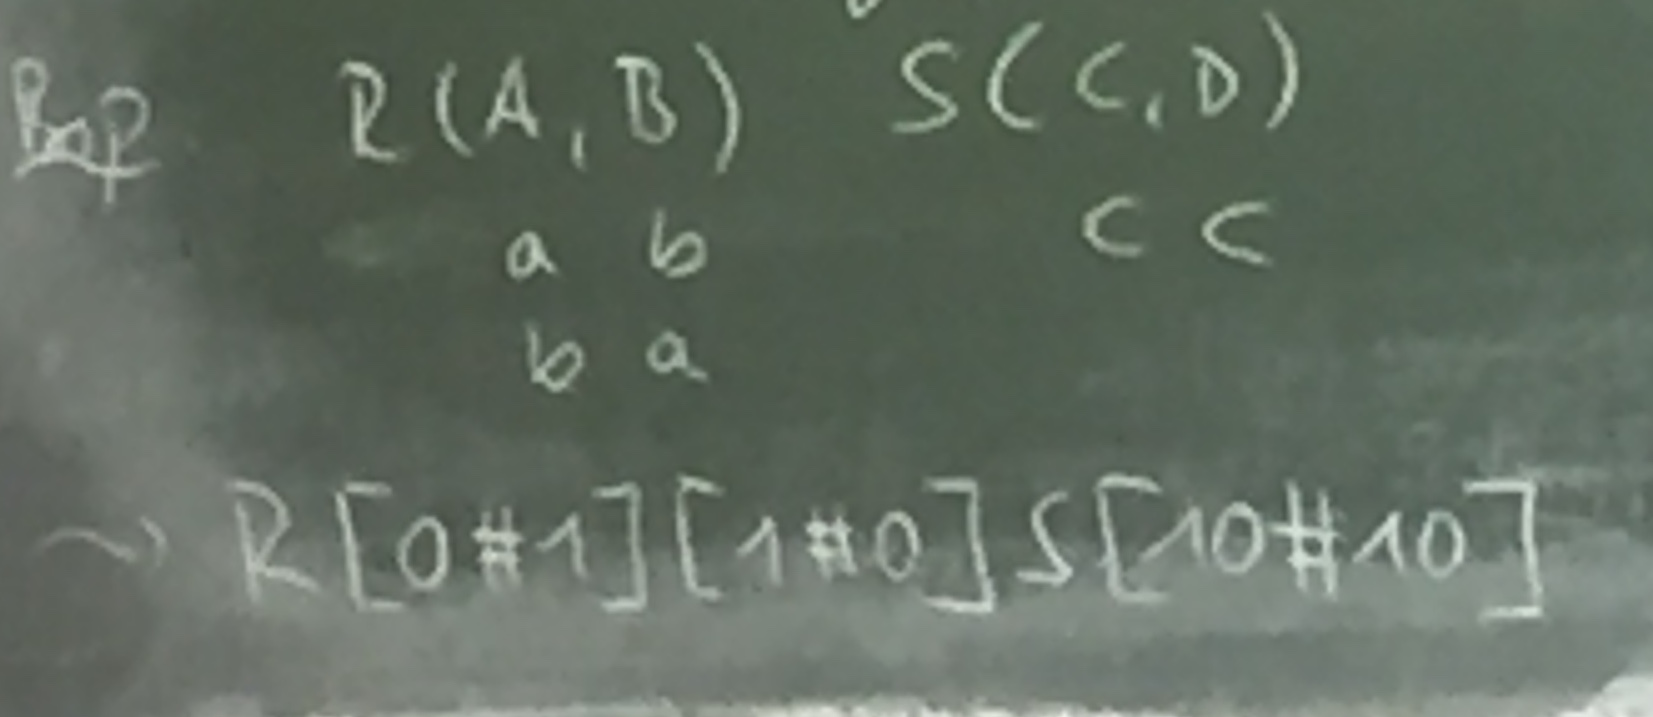
\includegraphics[width=0.7\linewidth]{img/img24}
\caption{}
\label{fig:img24}
\end{figure}


\subsection*{Satz 2.9}
Kalkülanfragen (RA-Anfragen) sind in QLOGSPACE

\paragraph{Beweis} Sei q eine DRC-Anfrage an ein DB-Schema $\sigma$ mit Antworttyp $\beta$ konstruierte TM $T_q$, die das Erkennungsproblem für q löst, wobei die Länge des Arbeitsbandes logarithmisch durch die Länge des Eingabebandes beschränkt ist.

\paragraph{Annahme:} $T_q$ startet mit $code_E(z)\#code_E(t)$ auf Eingabeband, $z \in \phi\sigma, t \in DOM^\beta_z$ (mit Konstanten aus z bildbare Tupel über $\beta$). E Aufzählungsfunktion für $DOM_Z$, q in Pränexnormalform mit Typ $\beta$. Zeige durch Induktion über die Anzahl der Quantoren von q. Berechnung kann mit $K \cdot  |code_E(z)\#code_E(t)|$, K Konstatne, Felder des Arbeitsbandes erfolge.

\paragraph*{Beispiel}
\begin{figure}[h!]
\centering
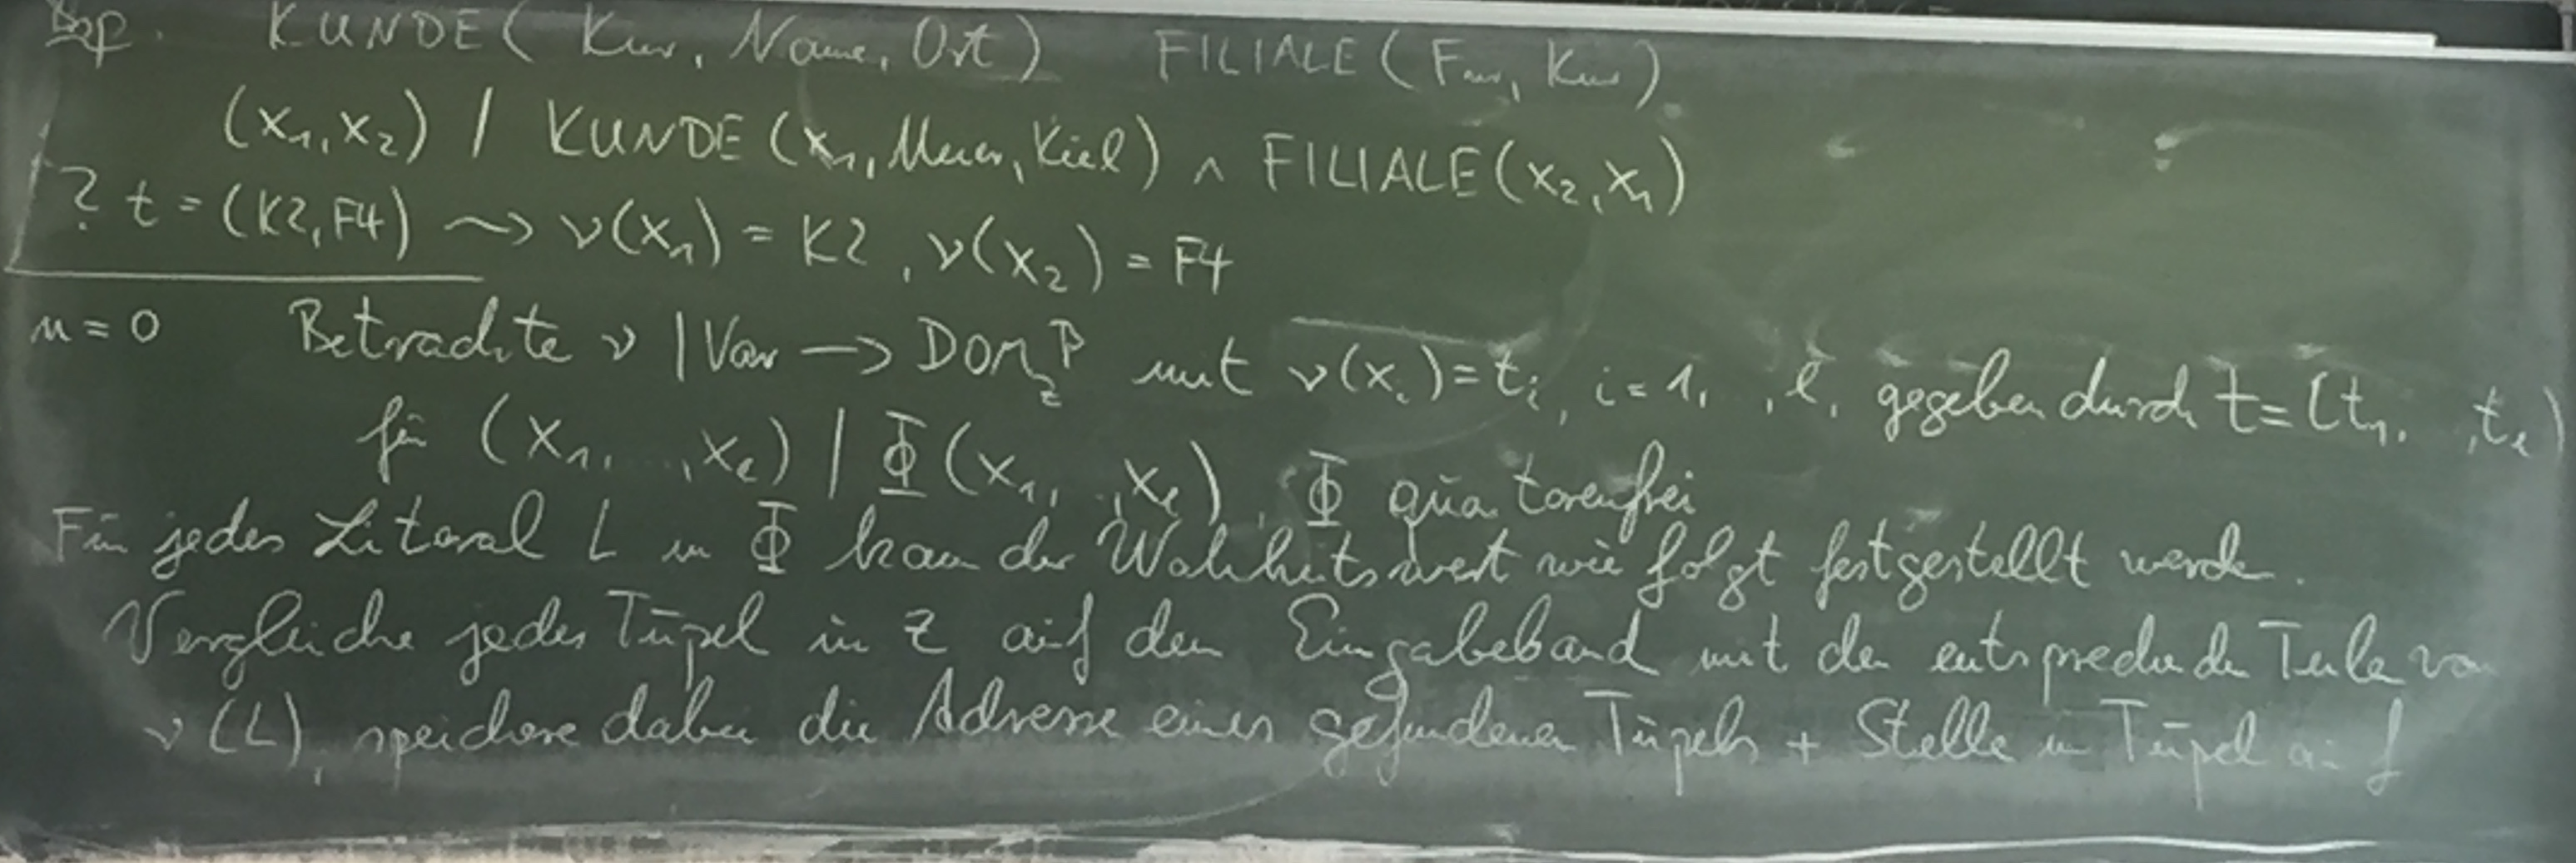
\includegraphics[width=0.7\linewidth]{img/img25}
\caption{}
\label{fig:img25}
\end{figure}
\begin{figure}[h!]
\centering
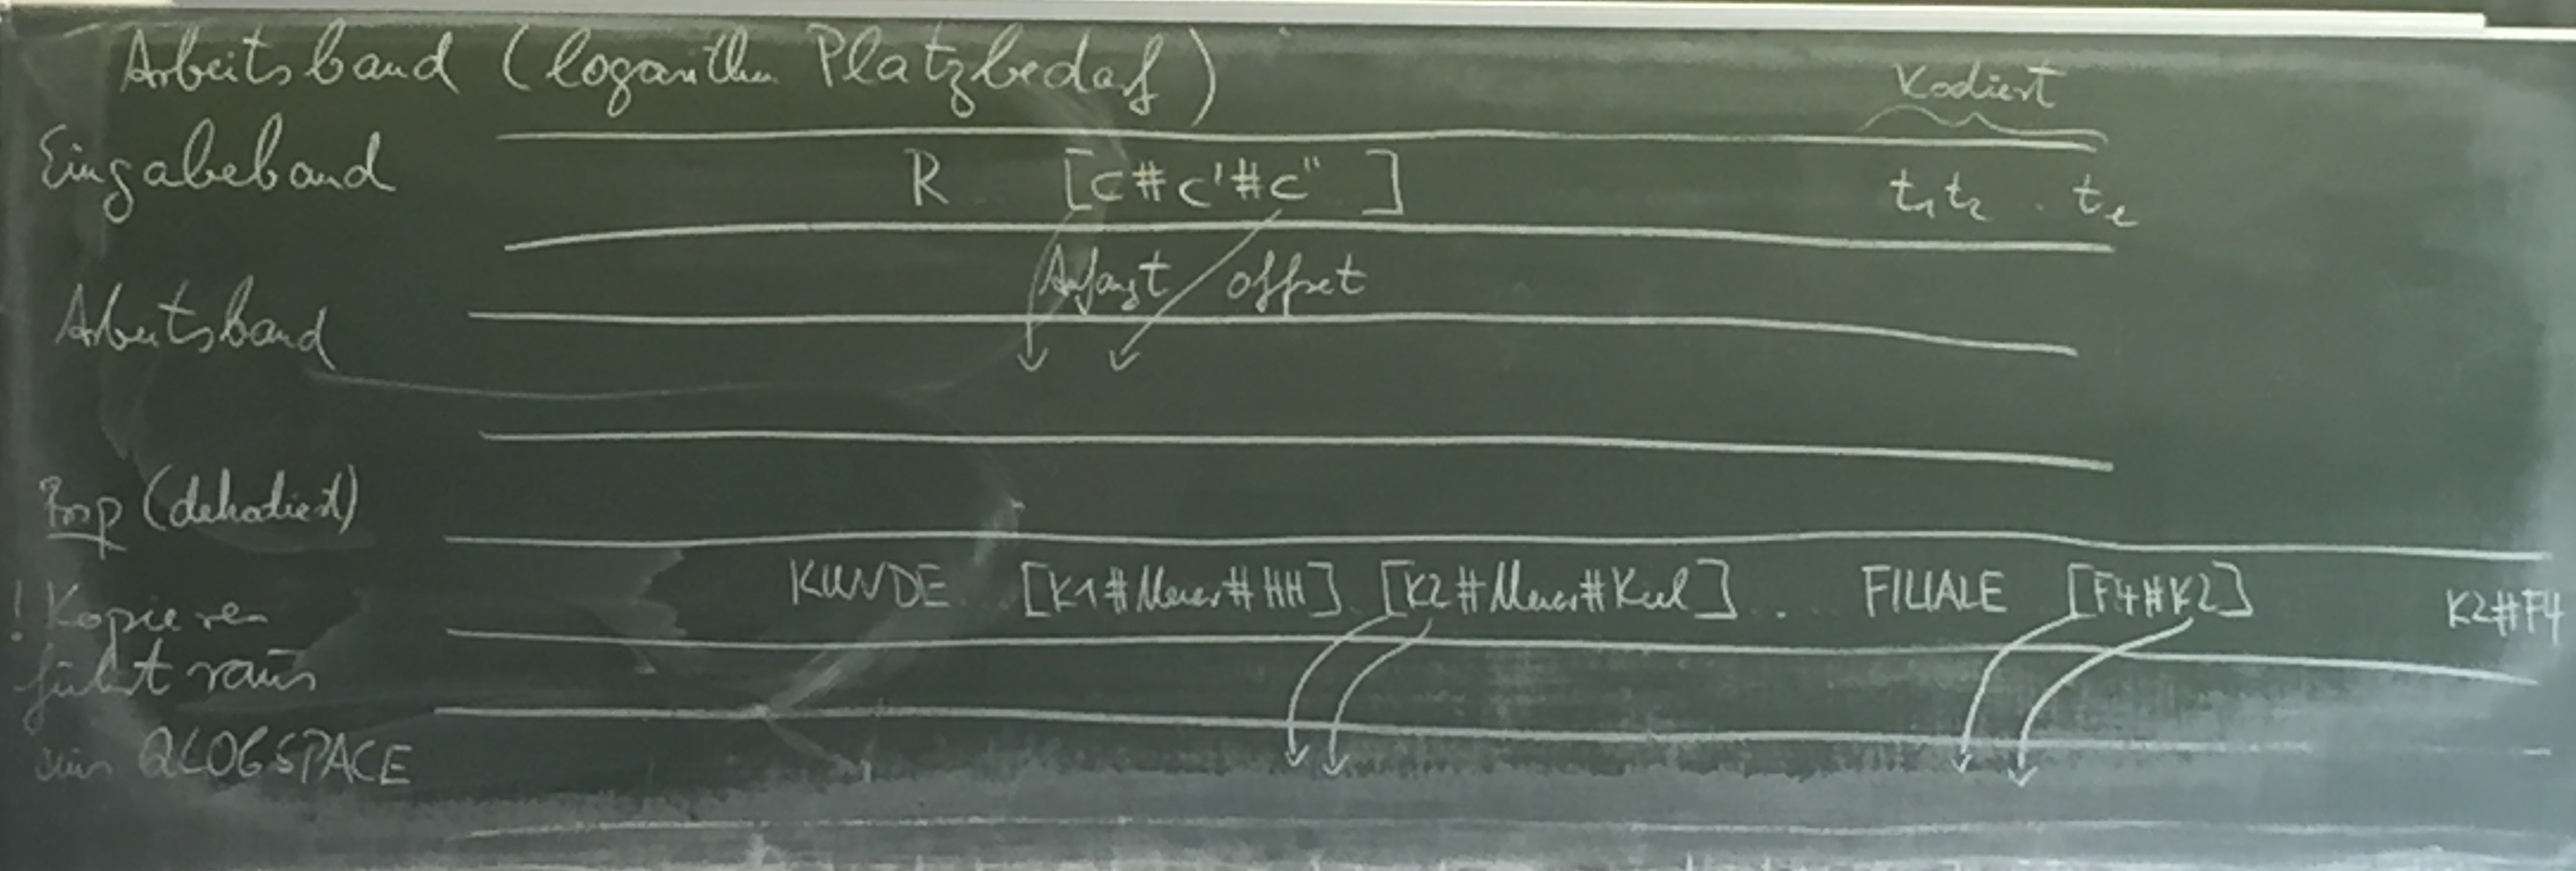
\includegraphics[width=0.7\linewidth]{img/img26}
\caption{}
\label{fig:img26}
\end{figure}

\paragraph{Induktionsannahme}
Jede Anfrage in PNF mit weniger als n Quantoren kann in LOGSPACE ahsgewertet werden.

\paragraph{Induktionsschluss}
$n-1 \rightarrow n$: $\phi$ habe n Quantoren und sei in der Form $(\exists x)(\Phi(x))((\forall x)(\Phi'(x))$

\paragraph{Idee}
Belege x mit den Konstanten auf dem Eingabeband in der Reihenfolge ihres Vorkommens (beschränkte Interpretatoin) für Merken einer solchen Konstante notwendig: $log(DOM_z)$ Felder:
\begin{align*}
&log(|DOM_z|) \le log(|code_E(z)\# code_E(z) \# code_E(t)|)
\end{align*}
%TODO: Extract definitions here

Nach Induktionsannahme: $\Phi'$ kann mit $K \cdot log(|code_E(z)\#code_E(t)|)$ Feldern ausgewertet werden $\leadsto$ vollständige Berechnung kann mit $(K + 1) \cdot log(|code_E(z) \# code_E(t)|)$ Feldern durch geführt werden. \\

Even in QLOGSPACE, aber nicht in DRC ausdrückbar $\Rightarrow$ Welche Anfragesprache entsrpicht genau QLOGSPACE? \\

\paragraph{Problem} Ohne gegebene Ordnung auf Wertebereich (bzgl. eine Nachfolgerelation) ist bis jetzt keine solche Sprache bekannt. Dies gilt für alle Klassen innerhalb von P, P eingeschlossen. In Klassen oberhalb von NP: Ordnung kein Problem, da in Sprache selbst ausdrückbar $\leadsto$ Annahme: Ordnung auf $DOM_z$, z Zustand. \\

Ordnung gegeben durch Relation NF(Vor, Nach), Nachfolgerrelation. DB-Schema entsprechend ergänzt $\Rightarrow DOM_Z \subseteq \mathbb{N}$ annehmbar mit 0 als minimales Element und m als maximales Element. Betrachte Operator trans (transitive Hülle):
Sei $\Phi(\overset{\rightarrow}{x}, \overset{\rightarrow}{y}) $ ein DRC-Ausdruck, der eine Binärrelation auf K-Tupeln repräsentiert. $\Phi[Trans]$ bezeichne die reflexive, transitive Hülle von $\Phi$. Sei $DRC^{pos\_trans}$ die Anfragesprache die aus DRC entsteht, indem der Operator ``trans'' in nicht negierten Teilausdrücken erlaubt wird.

\subsection*{Satz 2.10}

QNLOGSPACE = $DRC^{pos\_trans}$

\paragraph{Beweisidee}

``$\supseteq$'' einfach: Falls $\Phi(\overset{\rightarrow}{x}, \overset{\rightarrow}{y})$ in QNLOGSPACE, dann auch  $\Phi(\overset{\rightarrow}{x}, \overset{\rightarrow}{y})[trans]$. Rate ein  $\Phi(\overset{\rightarrow}{x}, \overset{\rightarrow}{y})$-Pfad.\\

``$\subseteq'$' Ausdruck in $DRC^{pos\_trans}$ gesucht, der NLOGSPACE-TM M enstpricht. \\
2 wesentliche Ideen: 
\begin{itemize}
	\item Zustand von M kann mit logarithmischen Aufwand kodiert werden (mit endl. vielen Variablen)
	\item Mit trans-Operator können ausgedrückt werden:
	\begin{itemize}
		\item Addition ``x+y=z''
		\item Test eines bestimmten Bits in einem Wort auf ``1'' (on(w,j))
	\end{itemize}
\end{itemize}

$\leadsto$ Feststellbar was Kopf von M sieht \\
$\leadsto$ Durch DRC-Ausdruck darstellbar: NEXT($z_1, z_2$) $z_n$ Zustandsbeschreibungen von M, $z_2$ folgt aus $z_1$ mit einem Übergang\\
$\leadsto$ PATH($z_1, z_2$ ) darstellbar mit einer oder mehreren Anwendungen von trans \\
$\leadsto$ PATH($z_0, z_j$), $z_0$ Anfangs- \& $z_j$ Endzustand \\

Für QLOGSPACE: deterministischer trans-Operator genügt. \\
$dtrans: \Phi_d(\overrightarrow{x}, \overrightarrow{y}) =_{def.} \Phi(\overrightarrow{x}, \overrightarrow{y}) \wedge (\forall \overrightarrow{z})(\lnot \Phi(\overrightarrow{x}, \overrightarrow{z} \vee \overrightarrow{y} = \overrightarrow{z})$

\begin{figure}[h!]
\centering
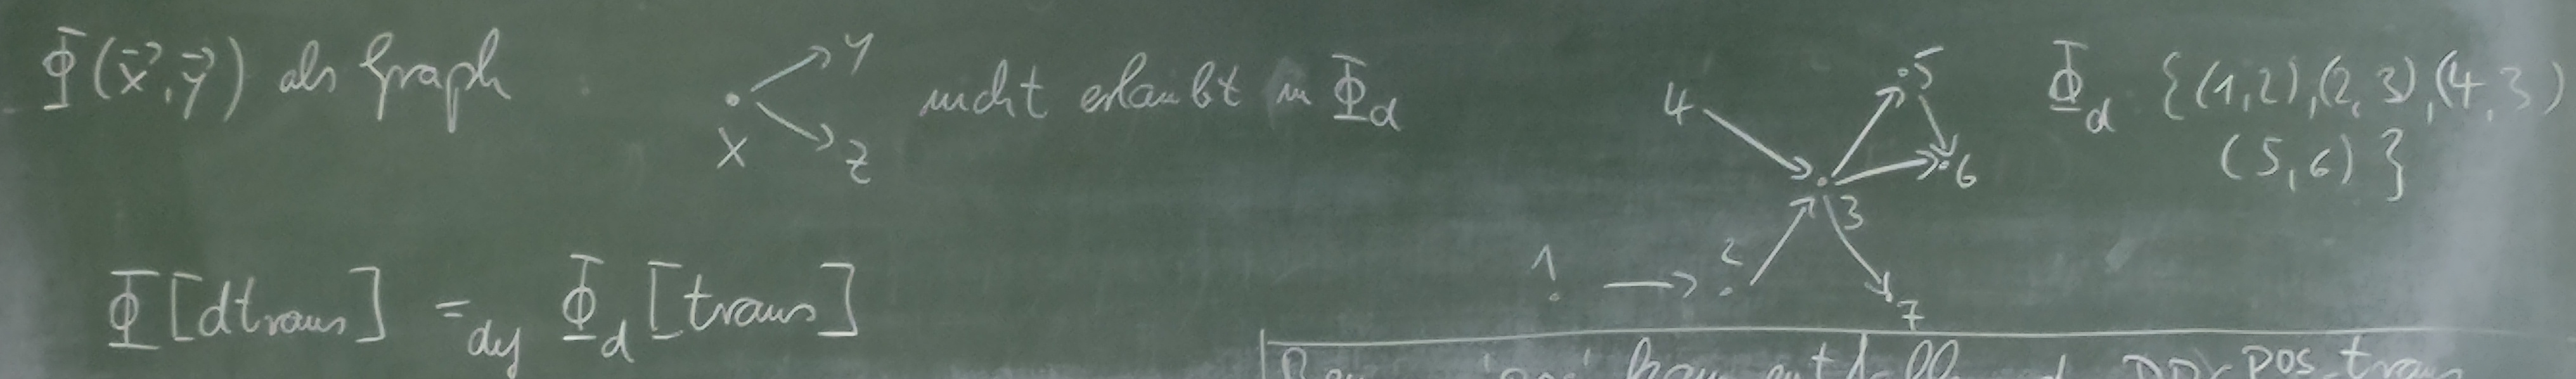
\includegraphics[width=0.7\linewidth]{img/img27}
\caption{}
\label{fig:img27}
\end{figure}


\paragraph{Bemerkung}

Pos kann entfallen, da $DRC^{pos\_trans}$ unter Negation abgeschlossen ist (gilt nur bei Vorhandensein einer Ordnung!)

\subsubsection*{Zusammenhang von Sprachklassen innerhalb von DRC}
Betrachte Anfragen der Form

\begin{align*}
&(x_1, \cdots, x_l) | (\exists y_1)\cdots(\exists y_k)(\Phi(x_1, \cdots, x_l, y_1, \cdots, y_k)), \Phi \text{ quantorenfrei} \\
& Q_\exists \text{ umfasst speziell die konjunktiven Anfragen:} \\
&(x_1, \cdots, x_l) | (\exists y_1)\cdots(\exists y_k)(\bigwedge_j R_j(u_{j1}, u_{jn_j}))\footnotemark
\end{align*}
\footnotetext{$u_{jn}$ Konstante oder Variable aus $\{ x_1, \cdots, y_k \}$}
Klasse der konjunktiven Anfragen ist Äquivalent zur Klasse der

\begin{itemize}
\item Datalog-Regeln ohne Rekursion: $R(x_1, \cdots, x_l) :- R_1(u_{11}, \cdots, u_{1n_1}), \cdots R_m(u_{m1}, \cdots, u_{mn_m})$
\item (einfache) Tableau-Anfrage (vgl. QbE mit Einschränkung)
\item RA-Anfragen mit positiver Selektion, Projektion (ohne Wiederholung), Join und Umbenennung
\item RA-Anfragen mit positiver Selektion, Projektion, Kreuzprodukt
\end{itemize}

Für Äquivalenz mit RA-Anfrage gefordert: ``Erfüllbarkeit, d.h. Anfragen dürfen nicht äquivalent sein zu''

\begin{align*}
q^\emptyset | \phi_\rho \rightarrow R_\beta \text{ mit } q^\emptyset(z) = \emptyset \text{ für alle } z \in \phi_\rho
\end{align*}

\subsection*{Erweiterung von Kalkülsprachen und Relationenalgebra}

\paragraph{a) DRC} Füge Fixpunktoperator hinzu (s.o.) \\ 
Fixpunktoperator partiell, d.h. nicht immer definiert, z.B. : $\Phi(R) = (x = 0 \wedge \lnot R(0) \wedge \lnot R(1)) \vee (x = 0 \wedge R(1)) \vee (x = 1 \wedge R(0))$

\begin{itemize}
	\item Inflationäre Semanktik $\leadsto DRC^{lfp+}$ 
	\paragraph{Definition: } Sei $\sigma' = \sigma \cup \{(S, \alpha_S), (S, \alpha_S) \not \in \sigma \}.$ \\ 
	$q(S) = (x_1, \cdots, x_{||\alpha_s}) | \Phi(x_1, \cdots x_{|\alpha_s|}) \text{ Anfrage zu } \sigma' \text { und } z \in \delta_\rho$ \\
	$lfp+(q(S))$ bezeichnet den Grenzwert der Folge $A_0, A_1, \cdots$ mit $A_0 = \emptyset_{\alpha_S}, A_i = A_{i-1} \cup \mu(q(S))(Z'), Z'(RT_i) = z(RT_i), (RT_i, \alpha_i) \in \sigma, Z'(S) = A_{i-1}$
	Offensichtlich: In PTIME, da monoton und jeden Zwischenergebnis Beschränkt durch $\sum^m_{i=1} |Dom|^{|\alpha_i|}$ beschränkt, m Anzahl der Relationstypen in $\sigma$.
	\item Nicht-inflationäre Semantik $\leadsto DRC^{lfp}$
	\paragraph{Definition} Wie oben bei lfp+ mit Unterschied $A_0 = \emptyset_{\alpha_j}, A_i = \mu(q(s))(z')$ \\
	Offensichtlich In PSPACE, in PTIME kann nicht gefolgert werden.
\end{itemize}

\paragraph{b) RA} Füge while-Anweisung hinzu (Schachtelungen erlaubt) vgl. QL. \\ Auch hier
\begin{itemize}
	\item Inflationär: Erzeuge Monotonie durch While Anweisungen der Form
\end{itemize}

\section*{Partielle Relationen}

\subsection*{Problemstellung}
Tupel im rDM bisher: $t: \alpha_i - U_j D_j$, d.h. t ist total definiert, Annahme ist für die reale Welt häufig nicht passend.

\begin{figure}[h!]
\centering
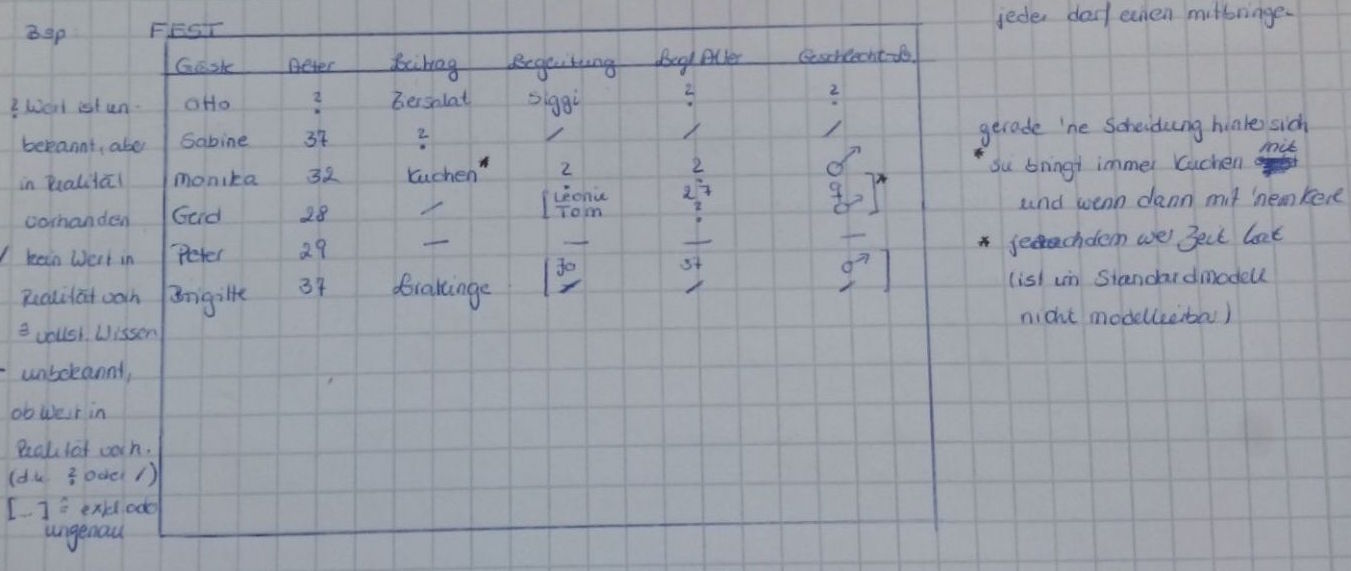
\includegraphics[width=0.7\linewidth]{img/img28}
\caption{}
\label{fig:img28}
\end{figure}

\paragraph{Zu ``$\backslash$'':}
Betrachte andere Schema: \texttt{GAST(Name, Alter, Beitrag), BEGLEITER(Name, B.Name, B.Alter, Geschickt Begl.)} + B.Name ist Schlüssel. \\
Gast ohne Begleitung: Entsprechendes Tupel fehlt in Relation Begleitung \\

\paragraph{Beachte:}
FEST in BCNF, da Gast und Begleitung zwei sich bedingende Schlüssel sind da restlichen Attribute sind alle durch die Schlüssel bestimmt.
$\leadsto$ Entwurfsproblematik ist bei verweis und partieller Information verschieden \\

Zeige Probleme bleiben bei geänderten Schema
\begin{itemize}
\item Gäste mit Begleitung, aber Angaben zur Begleitung aber teilweise oder völlig unbekannt oder nicht eindeutig
\end{itemize}

\paragraph{Betrachte TRC-Anfragen:} 
$(x) / GAST x \wedge \lnot (\exists y: BEGLEITER Y)(Y.Name = x.Name)$

\paragraph{Annahme:}
Alle Tupel sind total definiert
\begin{itemize}
\item clwa\footnote{Closed World Assumption}: ``Gib die Daten aller Gäste, die ohne Begleitung kommen''
\item mit owa\footnote{Open World Assumption}: ``Gib die Daten aller Gäste, zu denen in der Datenbank keine Begleitung angegeben ist''
\end{itemize}

\begin{figure}[h!]
\centering
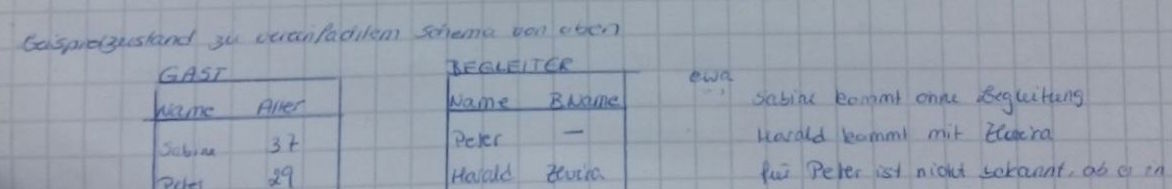
\includegraphics[width=0.7\linewidth]{img/img29}
\caption{}
\label{fig:img29}
\end{figure}

\paragraph{Problem:}
Eine Bedeutung von ``-'' ist ``Kein Wert vorhanden''
\begin{itemize}
\item Information zu Sabine und Peter gleich, aber unterschiedlich Repräsentiert
\item Anfrageauswertung
\end{itemize}


\paragraph{mögliche Auswege}: Kodierung von Information über Werte, z.B.: neues Attribut ``allein'' mit DOMAIN(allein) = $\{ $ ja, nein,unbekannt $ \}$. Beachte Integritätsbedingungen $\Rightarrow$ kein Eintrag mit gleichen Namen in Bedeutung erlaubt nur bei ja und unbekannt, bei nein gibt es keine Einschränkungen \\ 

$\Rightarrow$ Semantik kann nicht in der DB liegen!

\paragraph{Anfrage} (x) / GAST x $\wedge$ x.ALLEIN = ja (ist nicht mehr generisch!)
\paragraph{Problem} Kodierung von Information in / über Werte in den Werten selbst $\rightarrow$ Programmierung wird aufwendiger, verletzung der Generaly Property.

\paragraph{Datenbank} Entwurf an Annahme zu Weiten anpassen, fehlende Attributwerte vermeiden

\begin{figure}[h!]
\centering
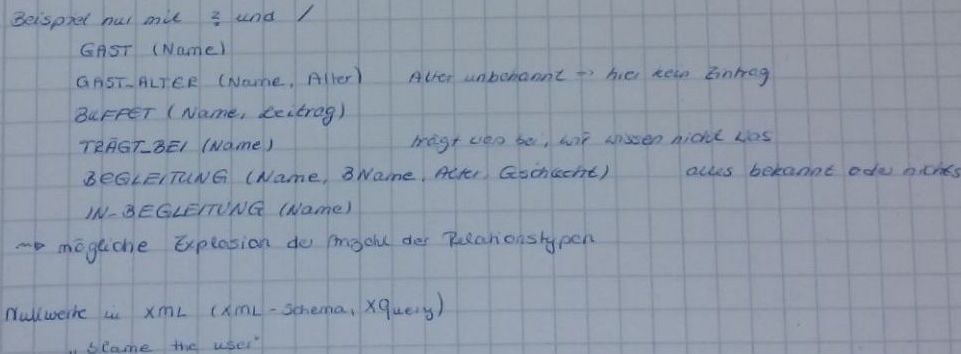
\includegraphics[width=0.7\linewidth]{img/img30}
\caption{}
\label{fig:img30}
\end{figure}

\subsection*{Nullwerte in XMl (XML-Schema, XQuery)}

``blame the user''- Prinzip (wie in COBOL) \\

\paragraph{Annahme:} Elemente in XML-Schema enhält Elemente Marke, Herstellungsjahr, Gefahrene Kilometer (optional). $\leadsto$ Folgende XML Darstellungen sind gültig:

\begin{verbatim}
<PKW><Marke>VW</Marke><HerstJahr>2016</HerstJahr><Gef-Km>25</Gef-Km></PKW>
\end{verbatim}
\begin{verbatim}
<PKW><Marke>VW</Marke><HerstJahr>2016</HerstJahr><Gef-Km /></PKW>
\end{verbatim}
\begin{verbatim}
<PKW><Marke>VW</Marke><HerstJahr>2016</HerstJahr></PKW>
\end{verbatim}

Anwendung legt Interpretation fest.

\begin{figure}
\centering
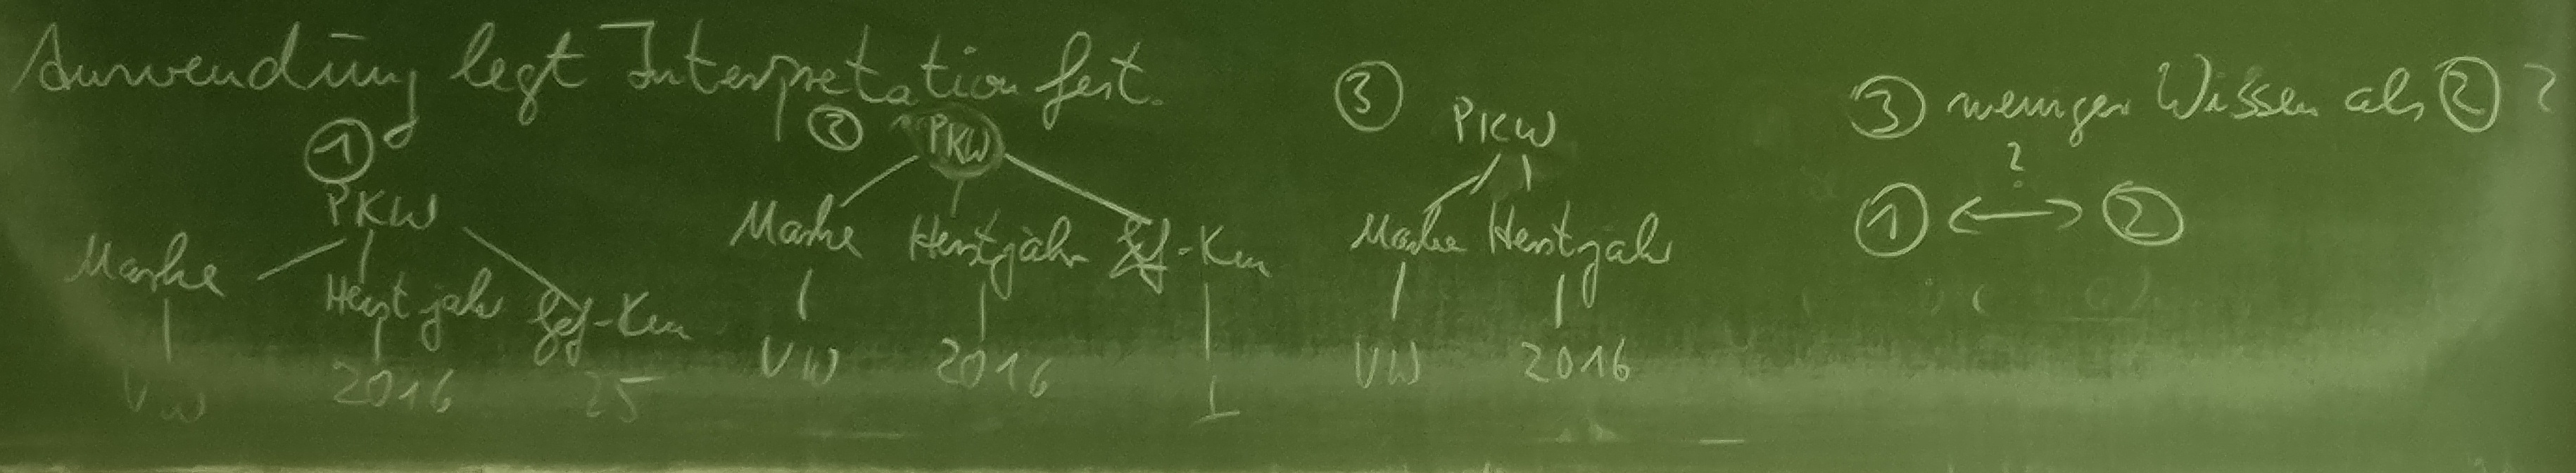
\includegraphics[width=0.9\linewidth]{img/img31}
\caption{}
\label{fig:img31}
\end{figure}


\paragraph{Fragen:}
\begin{itemize}
\item Darstellung?
\item Auswertung?
\item Ergebnisrepräsentation?
\end{itemize}

\subsection*{Modellierung unvollständiger Information}
\paragraph{Annahme:} Ein Symbol (``w'') zum Repräsentieren eines indifferenten Attributwerts. \\
w-Tupel: $t | \alpha_i \rightarrow \bigcup_{A \in \alpha_i} dom(A), \text{t(A) definiert oder undefiniert}$
w-Relation: Menge von w-Tupeln

\paragraph{Definition: Überdeckt (Tupel)}
Seien t,t' w-Tupel über $\alpha$: t' überdeckt t (t' ist eine Überdeckung von t), in Zeichen: $t' \ge t$, genau dann wenn 
\begin{align*}
(\forall A \in \alpha_i)(t(A) definiert \Rightarrow t'(A) definiert und t(A) = t'(A))
\end{align*}

Bsp: $(1,a,w) \ge (w,a,w)$

\paragraph{Definition: Überdeckt (Relation)}
Seien S,R w-Relationen über $\alpha$: R überdeckt S (R ist eine Überdeckung von S), in Zeichen: $R \ge S$, genau dann wenn
\begin{align*}
(\forall t \in S)(\exists t' \in R)(t' \ge t)
\end{align*} 

\paragraph{Vervollständigung eines Tupels}
\paragraph{1)}
\begin{figure}
\centering
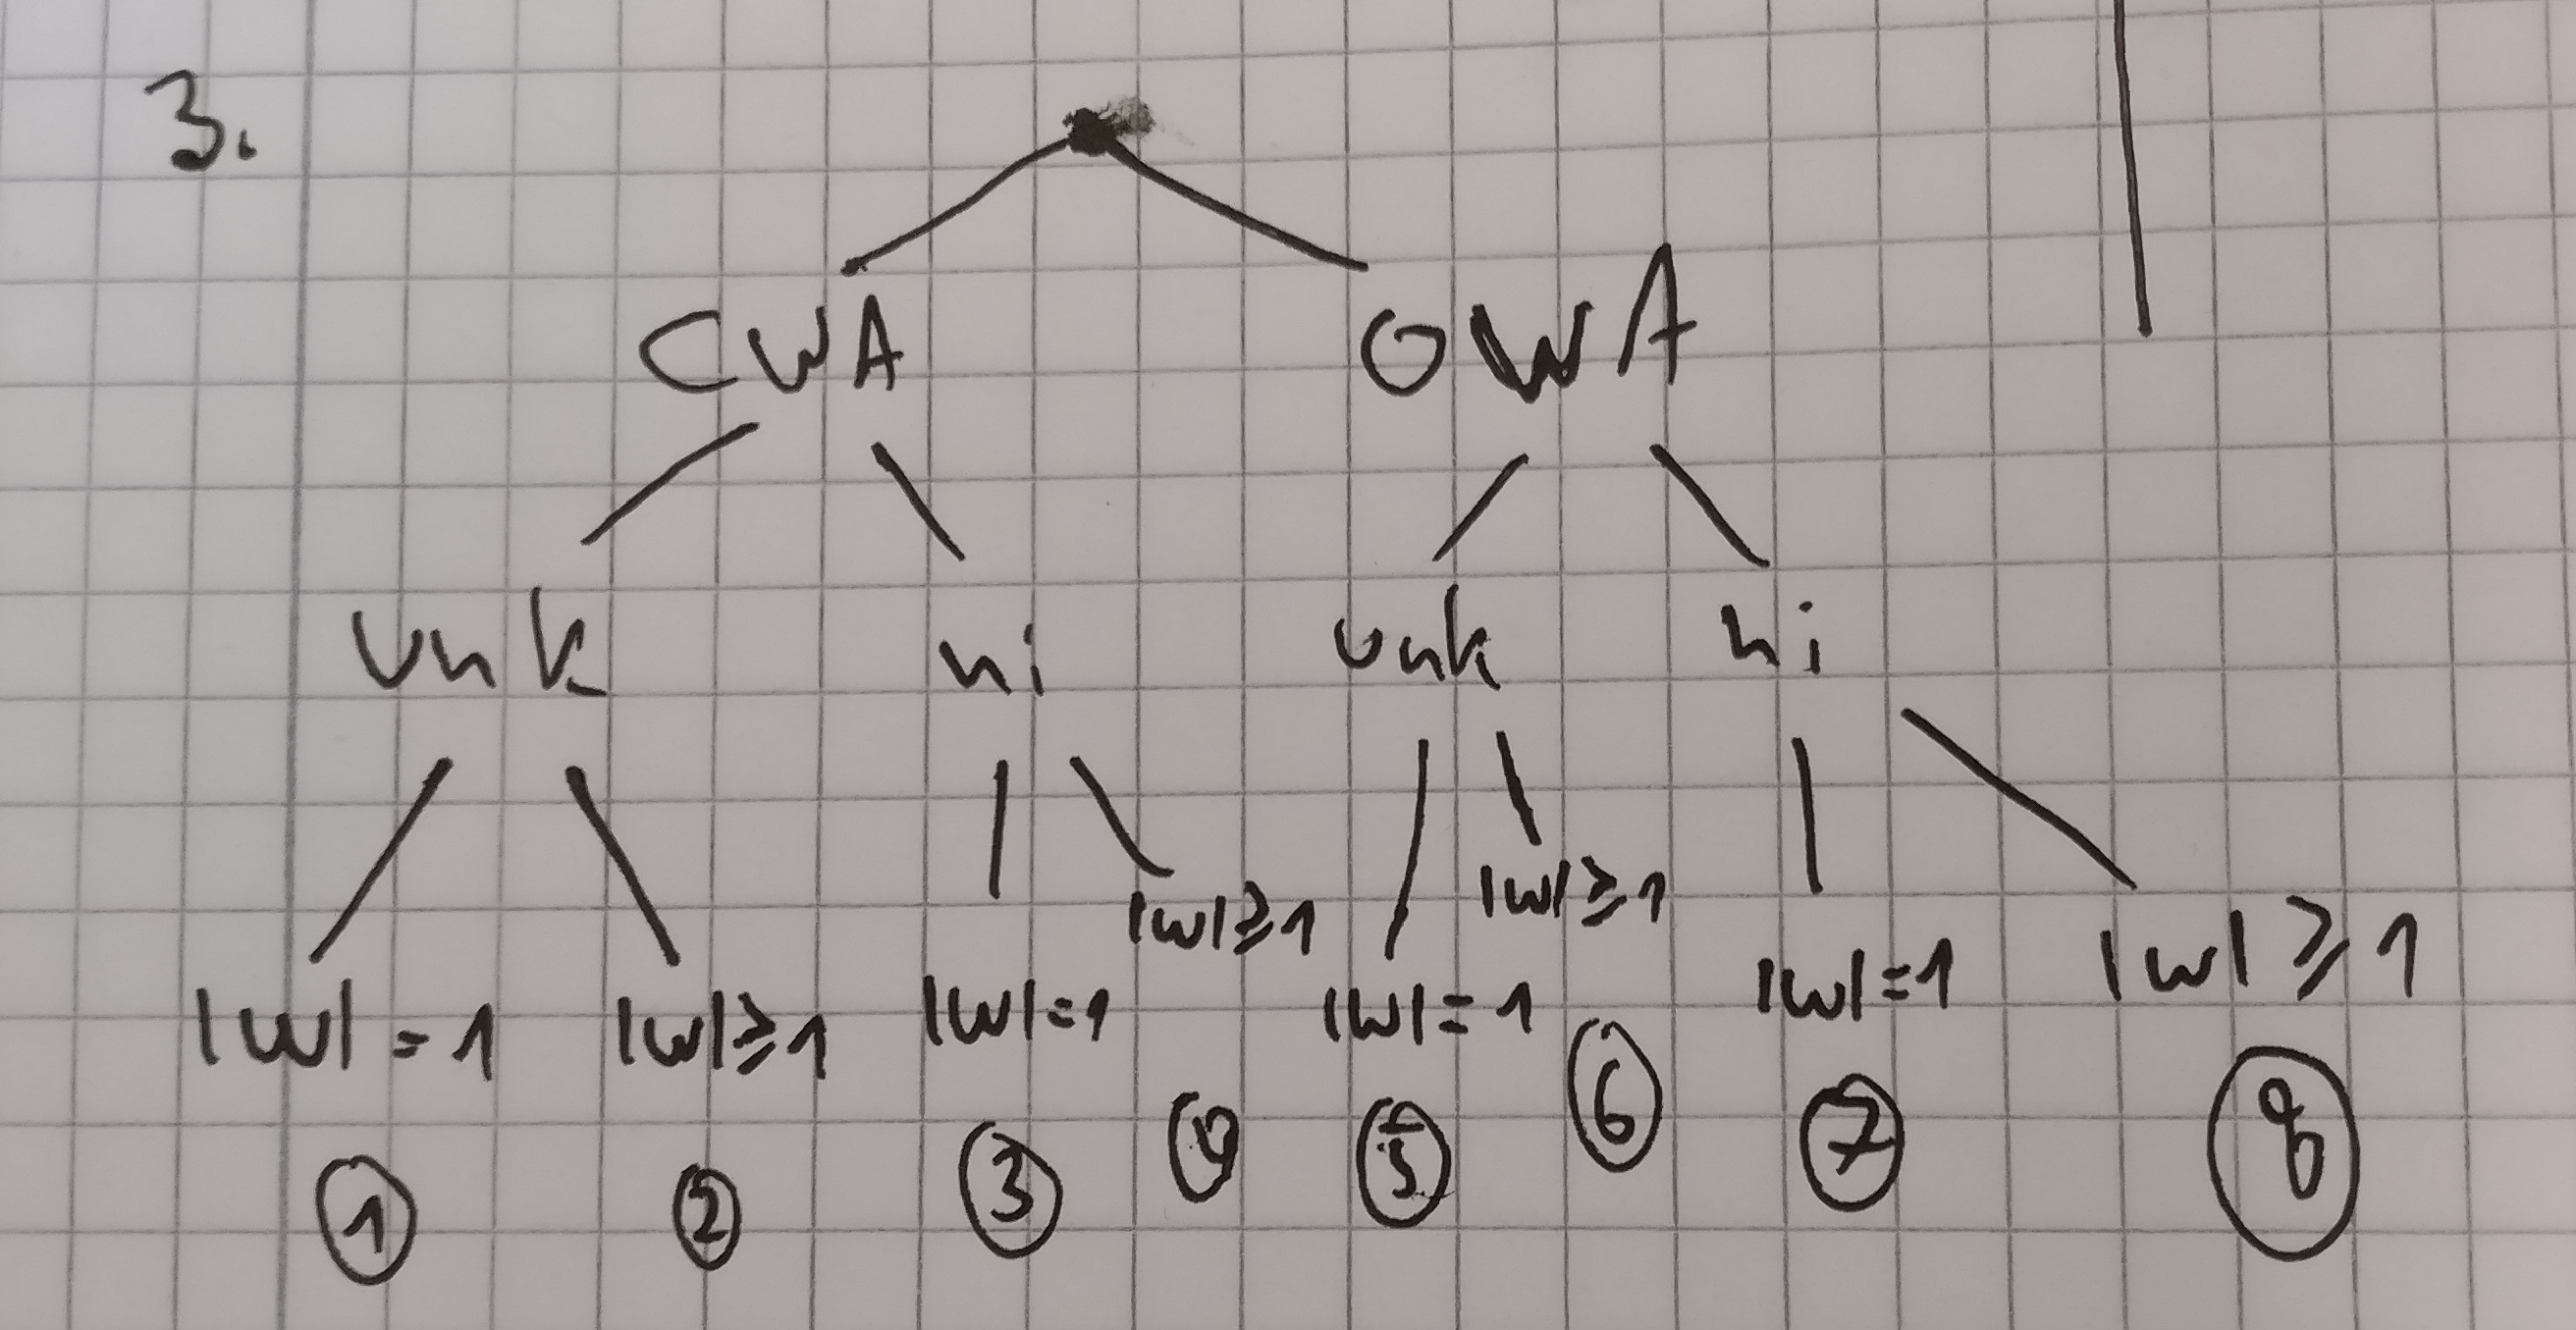
\includegraphics[width=0.7\linewidth]{img/img32}
\caption{}
\label{fig:img32}
\end{figure}

\begin{figure}
\centering
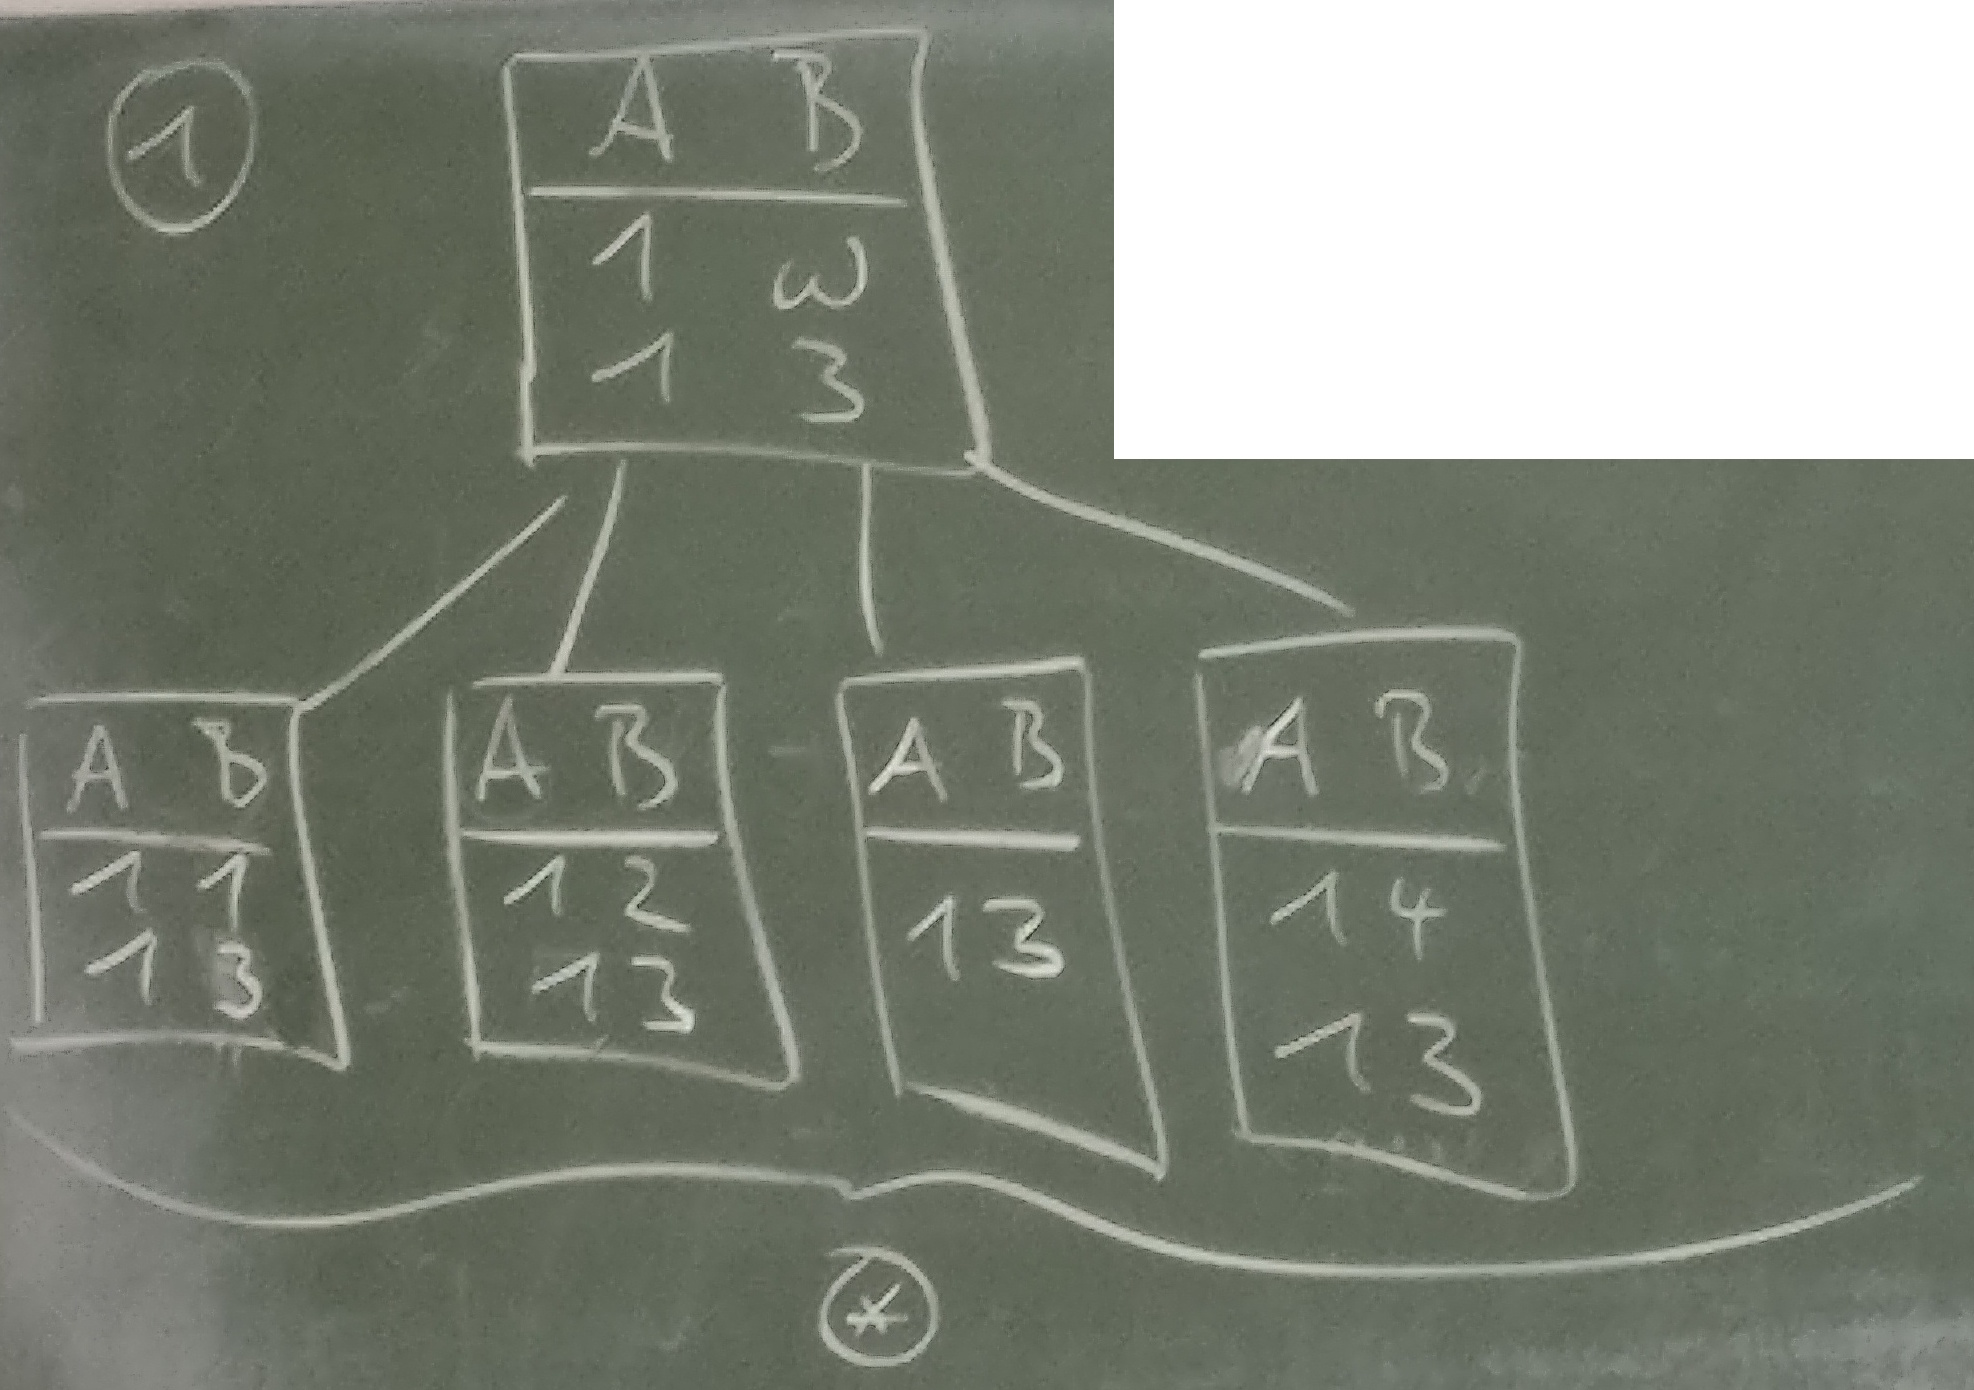
\includegraphics[width=0.7\linewidth]{img/img33}
\caption{}
\label{fig:img33}
\end{figure}

Ersetze jedes Vorkommen von w durch genau einen Wert: Vervollständigung (completion)

\paragraph{2)}
\begin{figure}
\centering
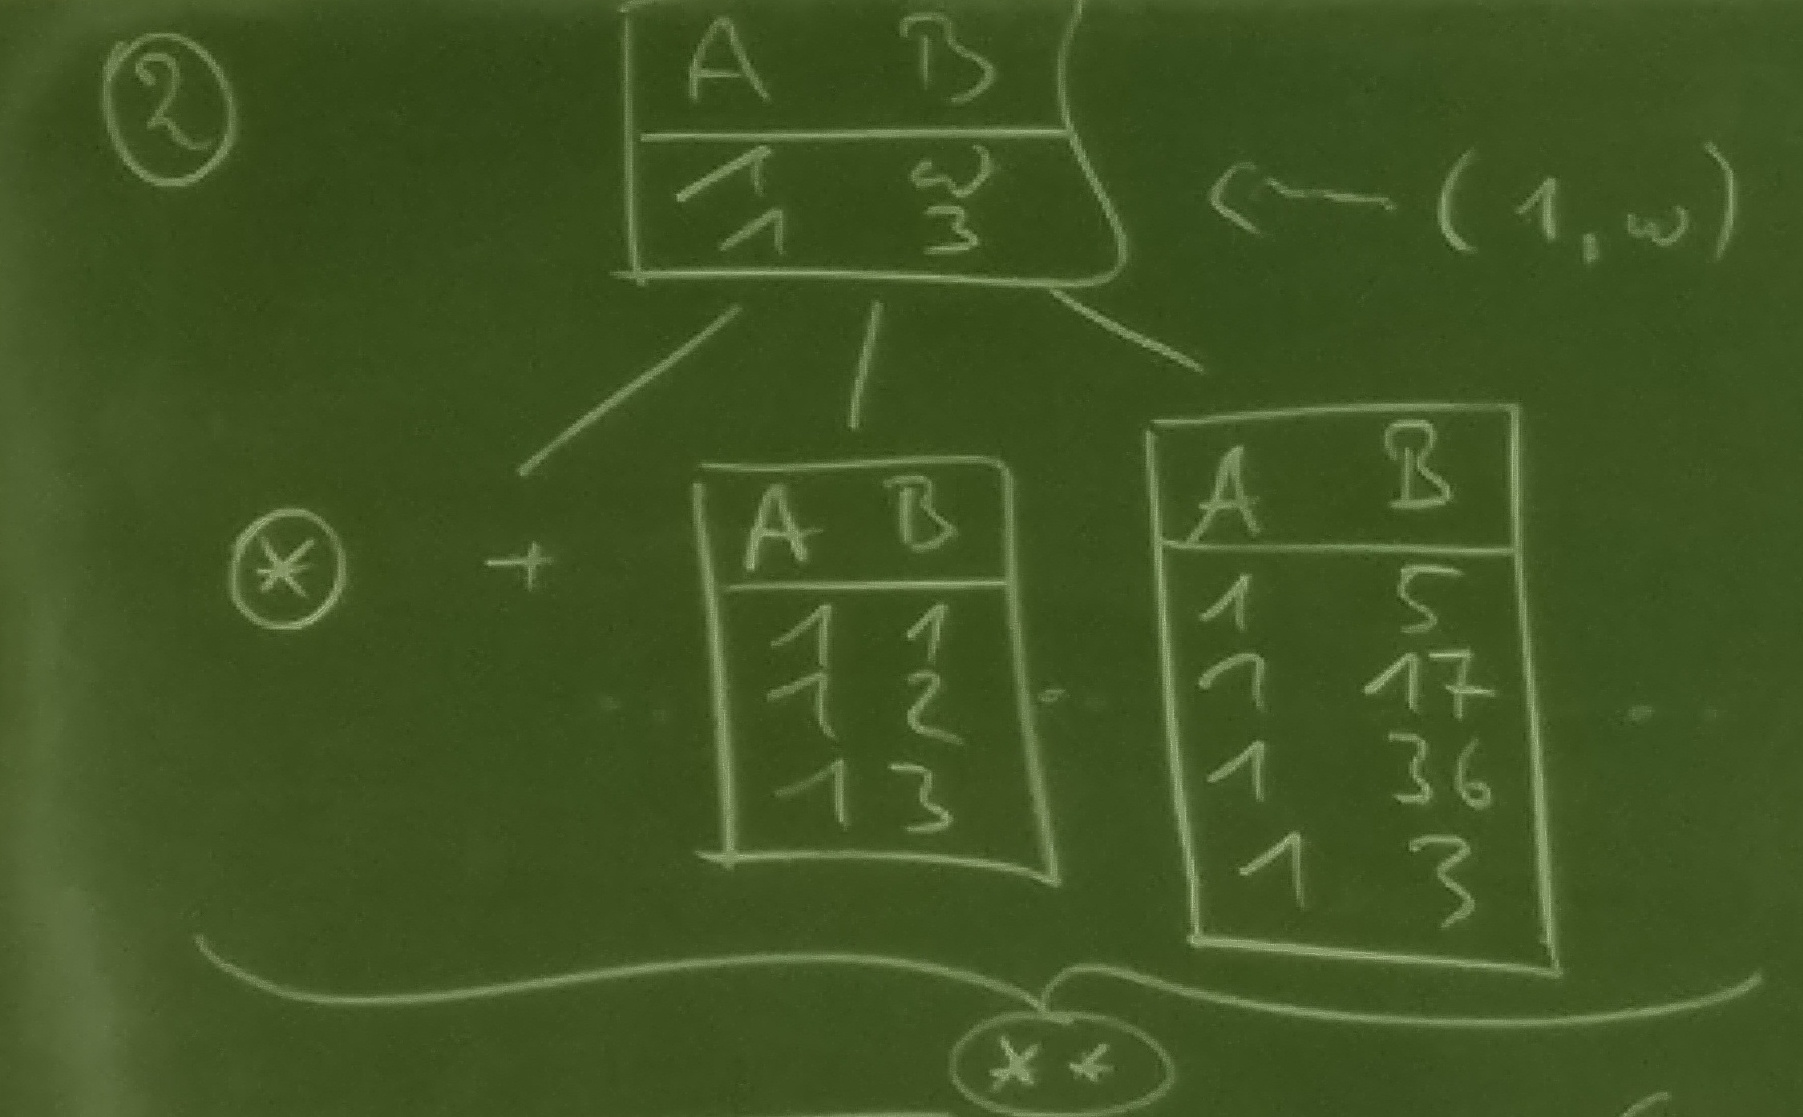
\includegraphics[width=0.7\linewidth]{img/img34}
\caption{}
\label{fig:img34}
\end{figure}

Ersetze w durch einen oder mehrere Werte: enge Auswertung (close extension)


\paragraph{3)}
\begin{figure}
\centering
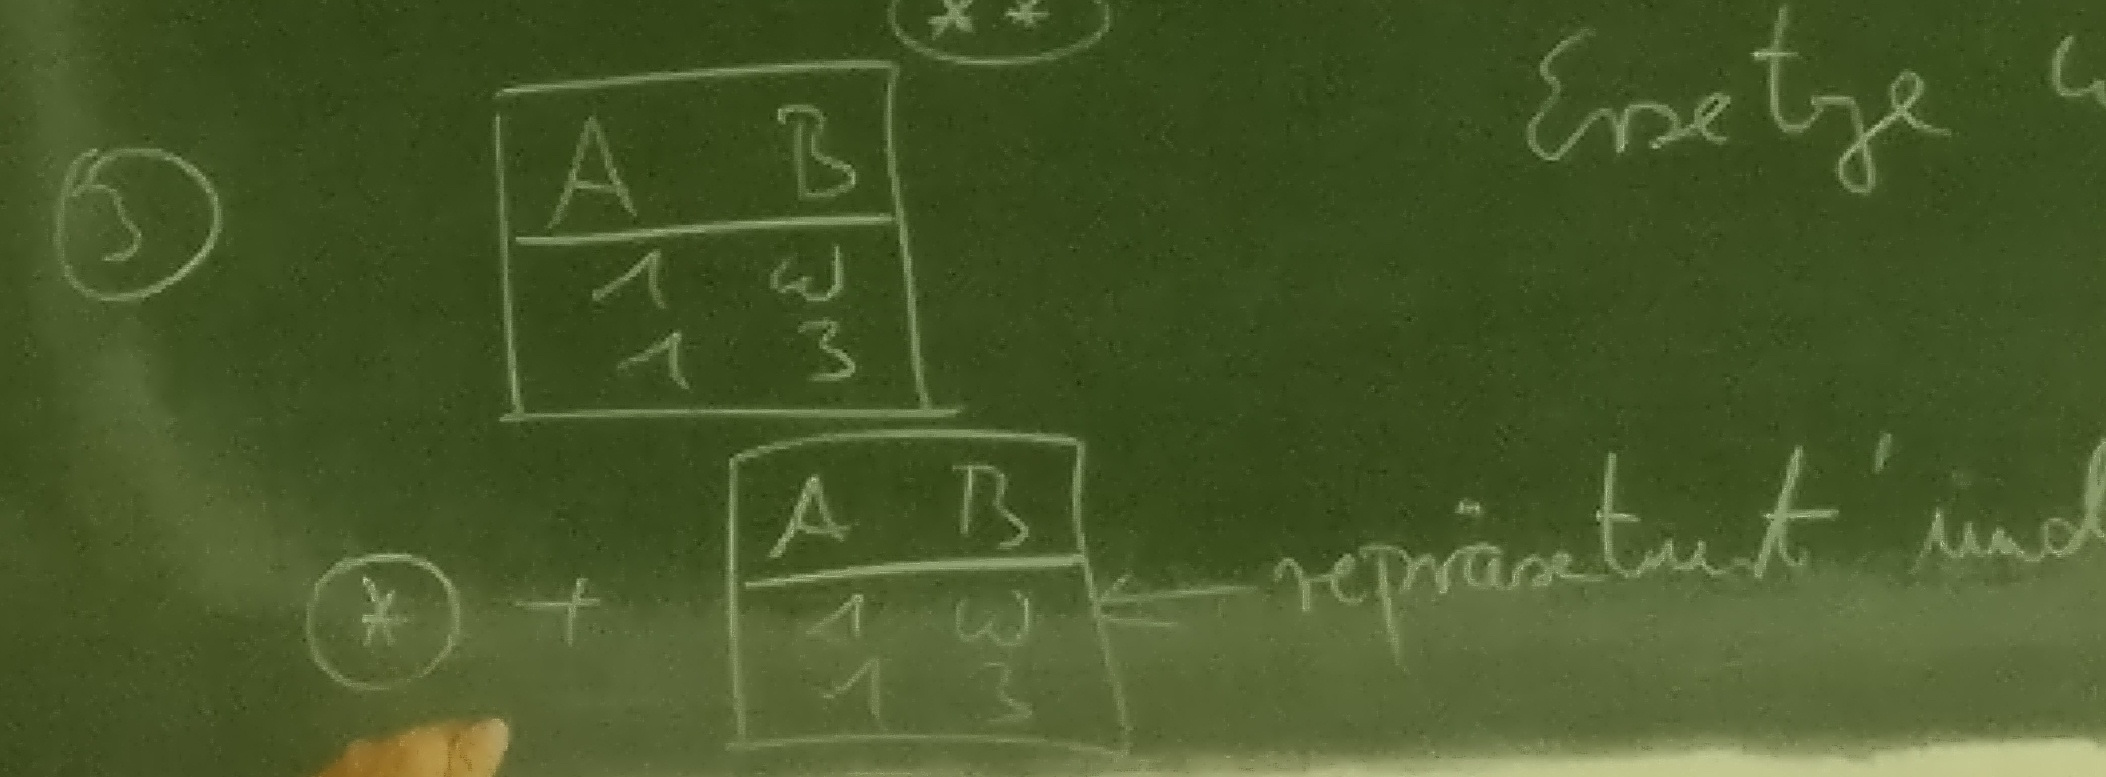
\includegraphics[width=0.7\linewidth]{img/img35}
\caption{}
\label{fig:img35}
\end{figure}

Ersetze w durch \textbf{einen} Wert oder durch ``undefiniert'' (entspricht ``nicht existent''): Erweiterung (augmentation)

\paragraph{4)}
\begin{figure}
\centering
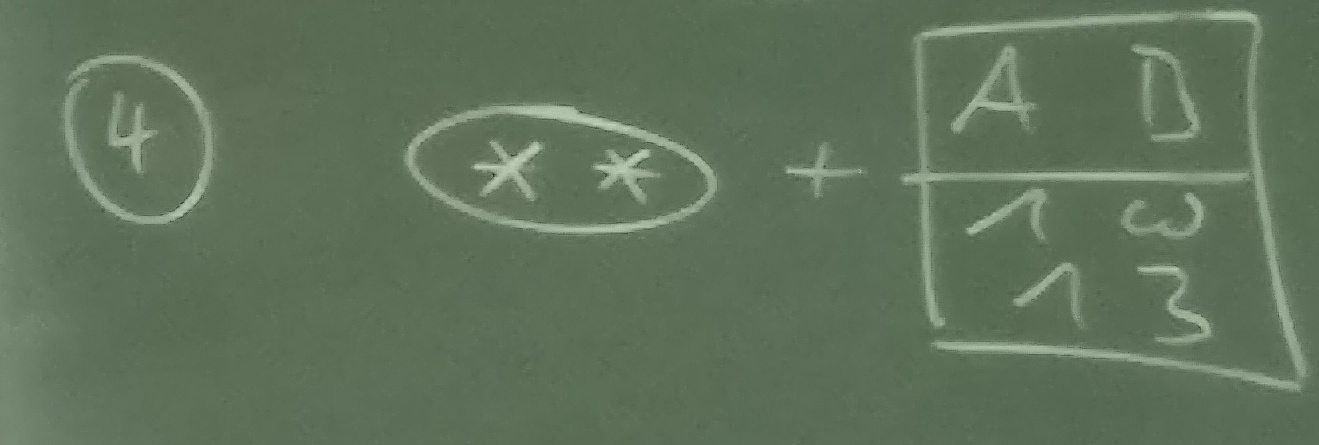
\includegraphics[width=0.7\linewidth]{img/img36}
\caption{}
\label{fig:img36}
\end{figure}

enge Überdeckung (close subsumption) \\

OWA: beliebige Tupel können hinzukommen

\begin{figure}
\centering
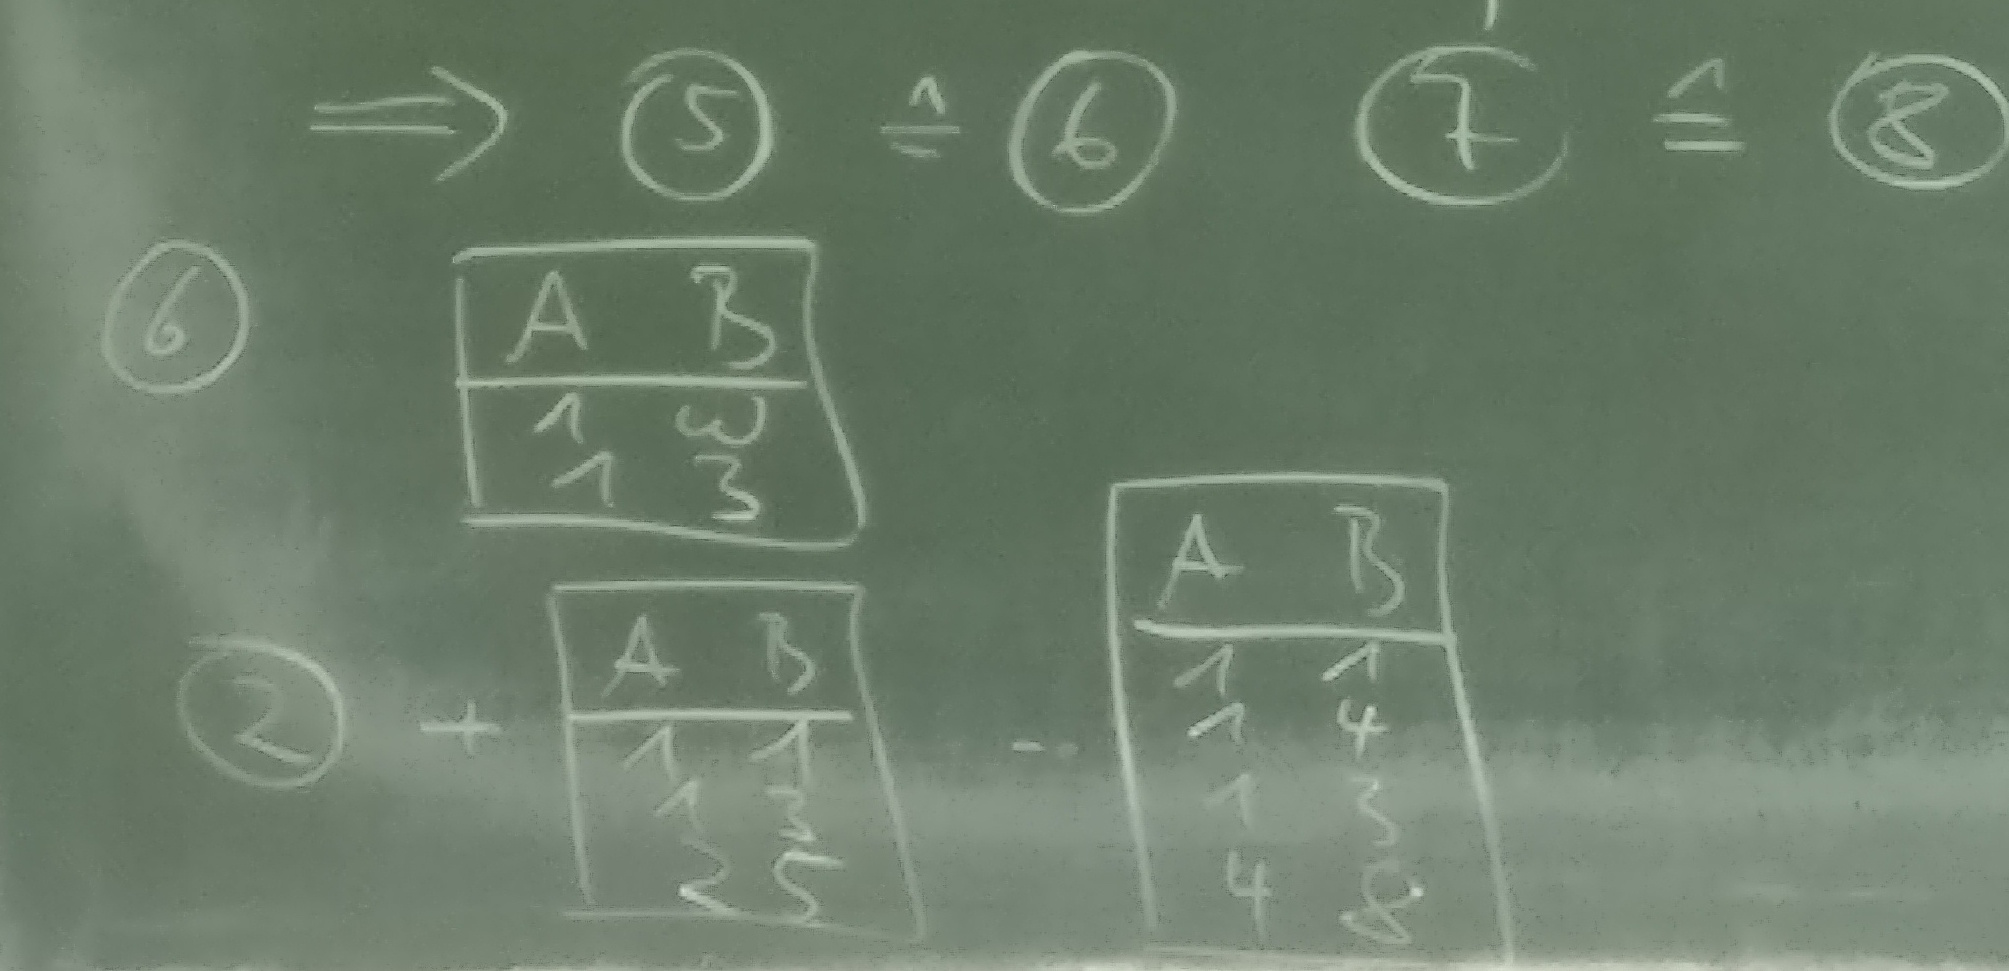
\includegraphics[width=0.7\linewidth]{img/img37}
\caption{}
\label{fig:img37}
\end{figure}

\begin{figure}
\centering
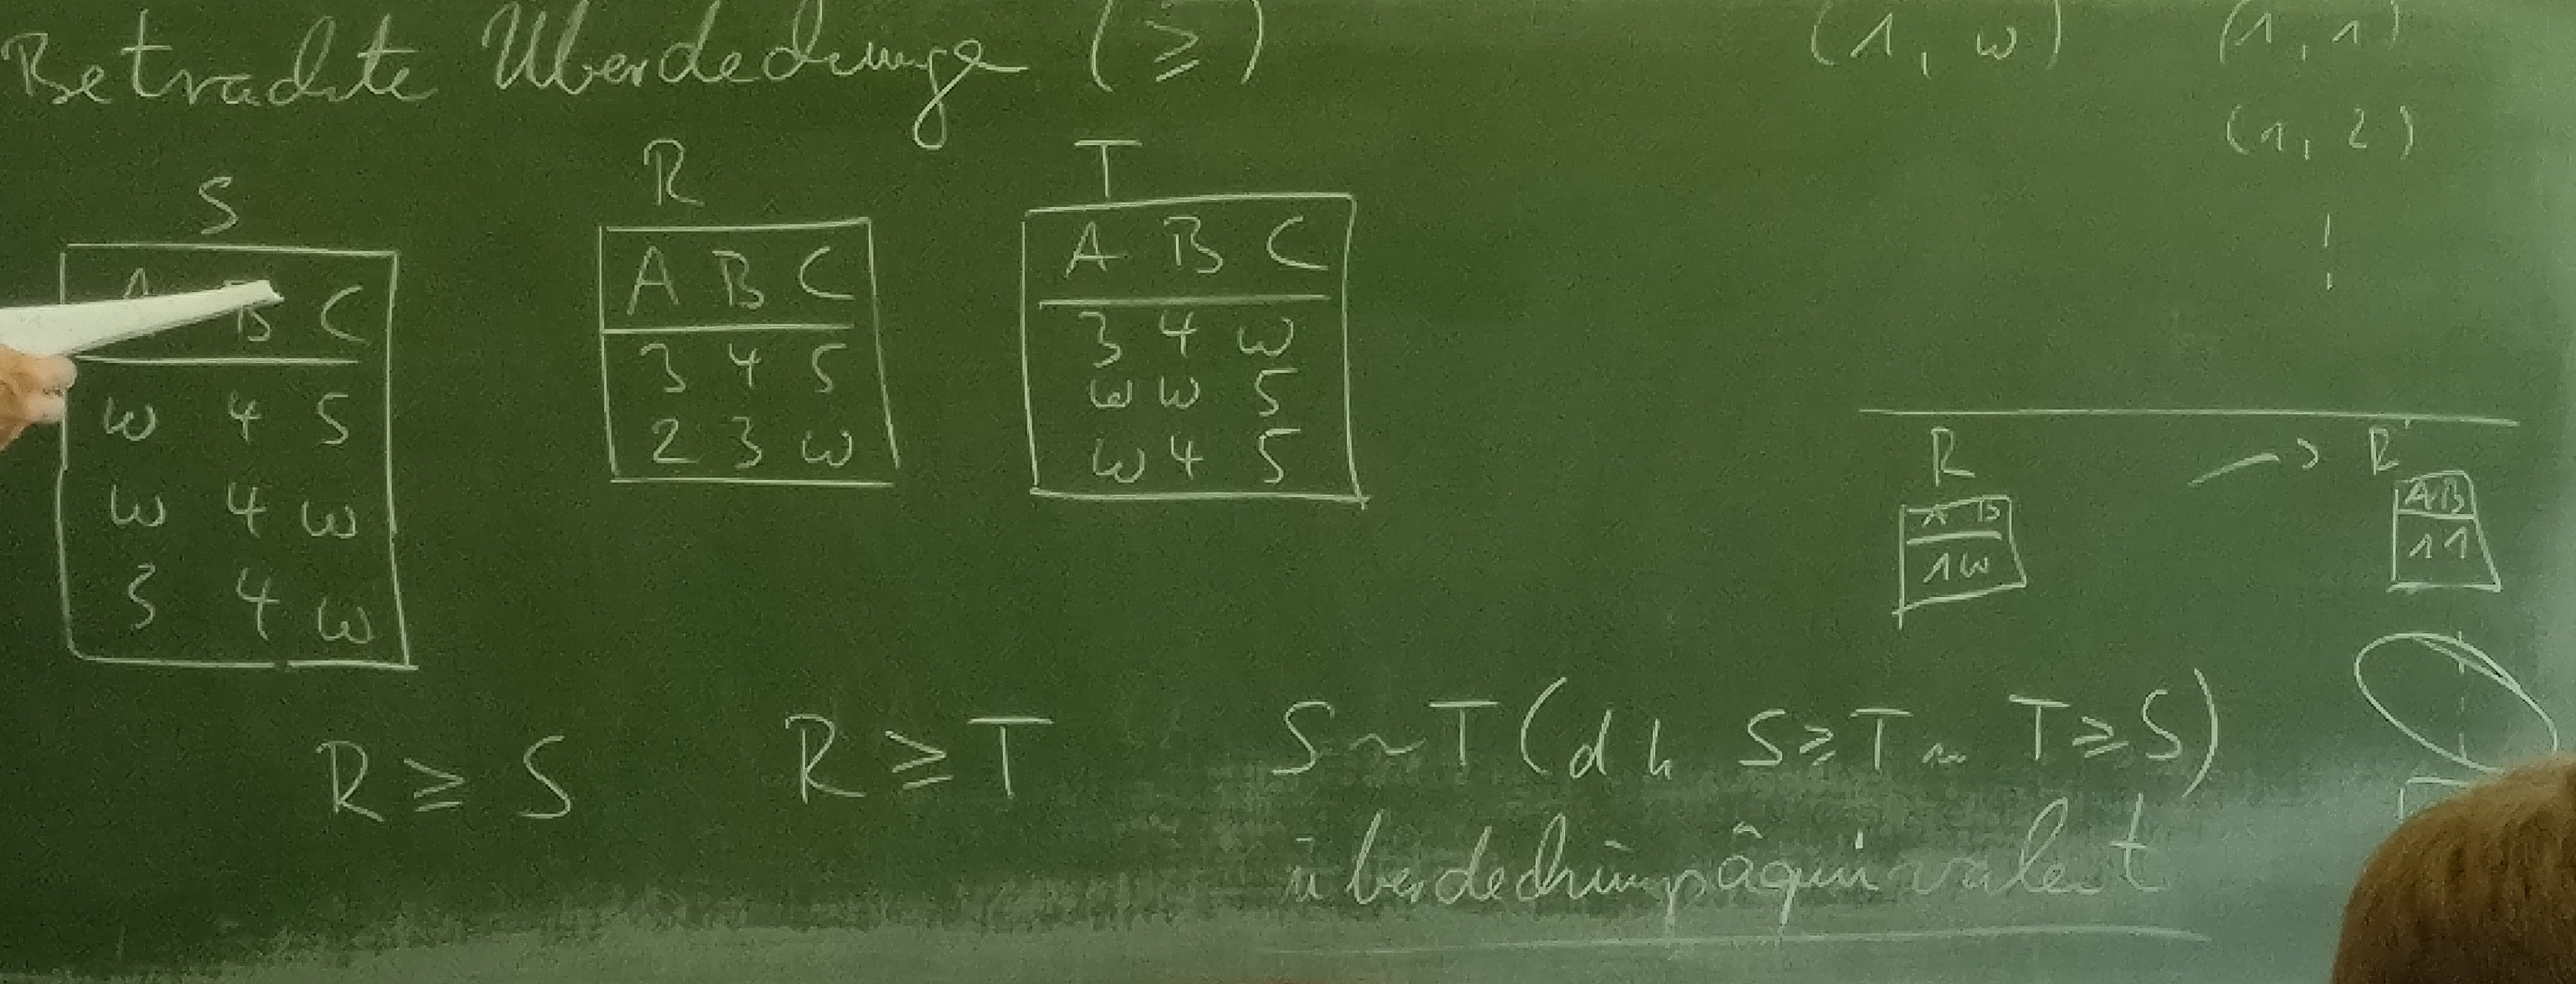
\includegraphics[width=0.7\linewidth]{img/img38}
\caption{}
\label{fig:img38}
\end{figure}

\paragraph{Anfragesprachen:} Annahme, Wert unbekannt, aber existiert

\paragraph{1)} Modellierung: w-Relation mit $|w| = 1$

\begin{figure}
\centering
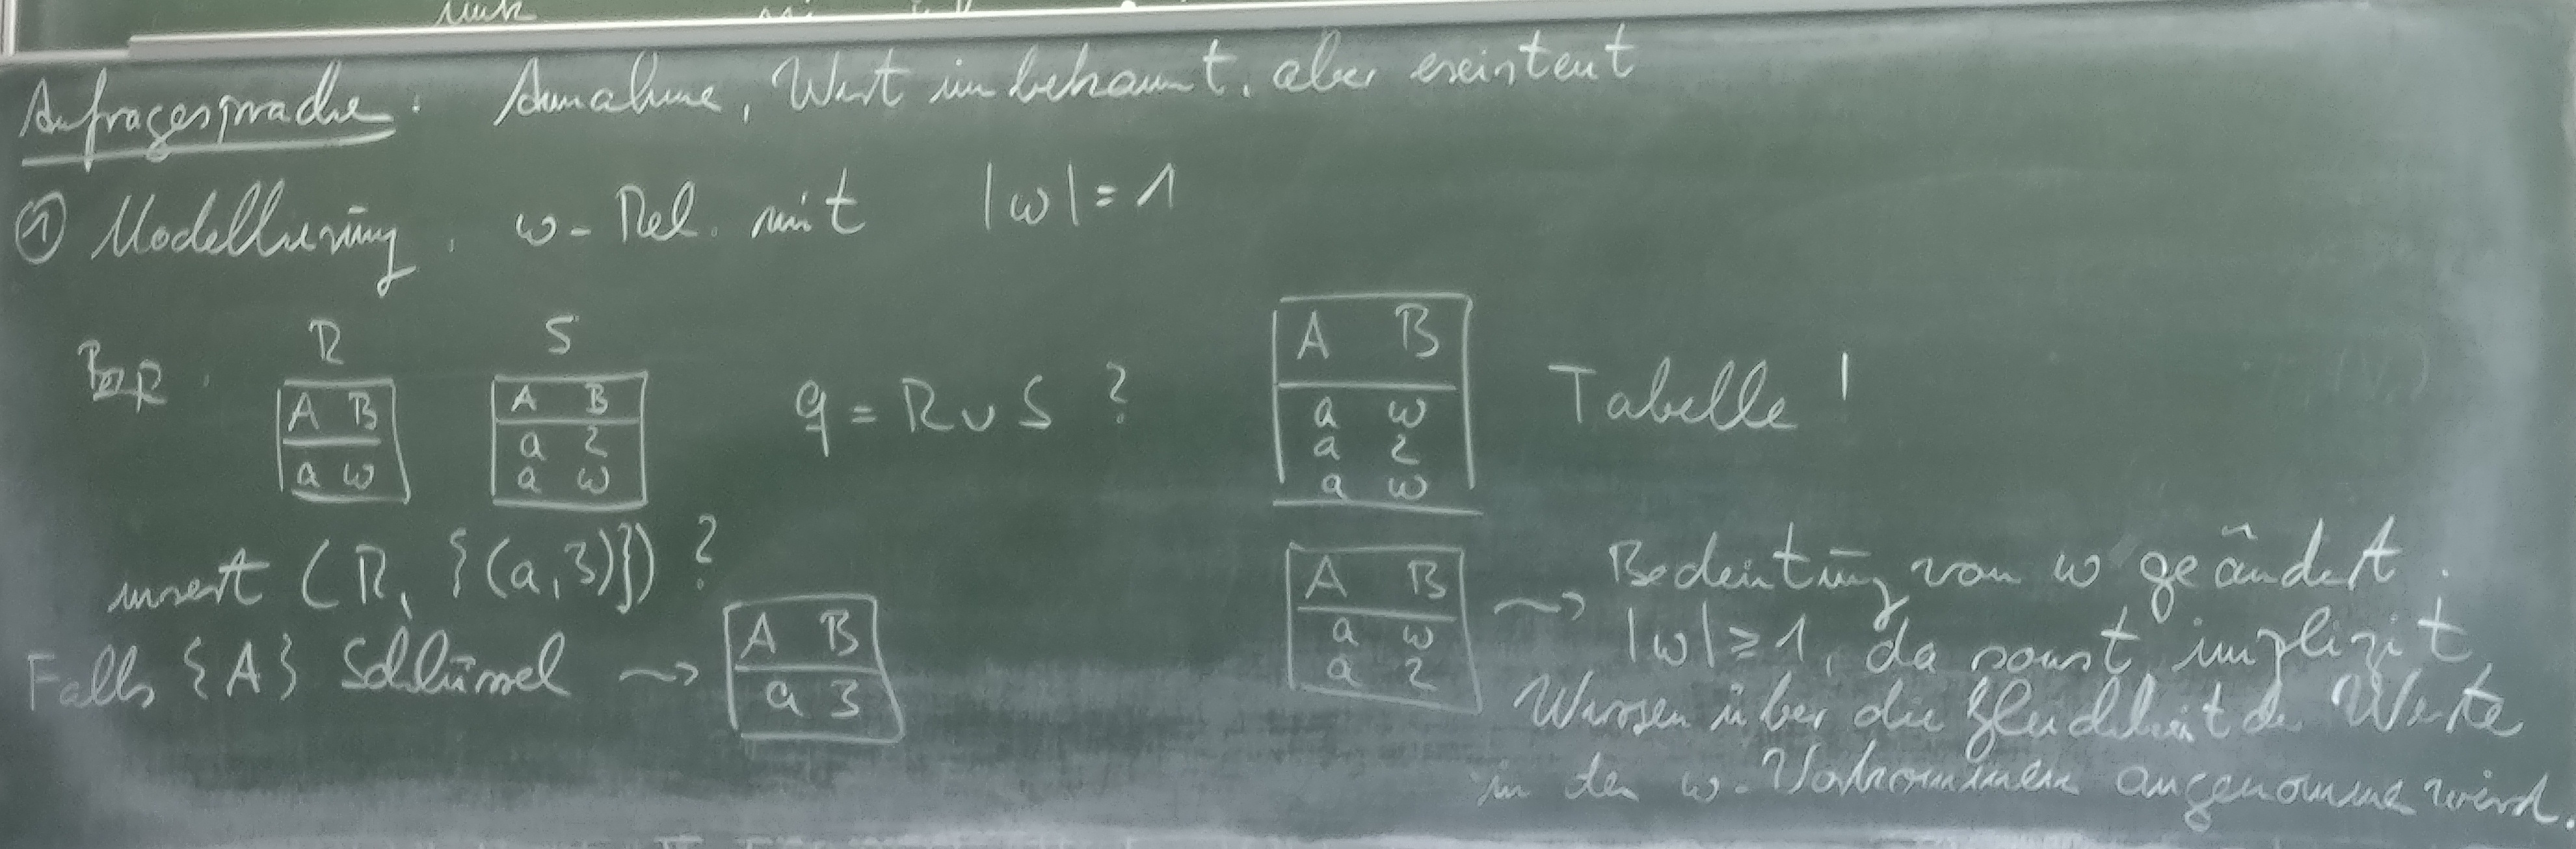
\includegraphics[width=0.9\linewidth]{img/img39}
\caption{}
\label{fig:img39}
\end{figure}


\begin{figure}
\centering
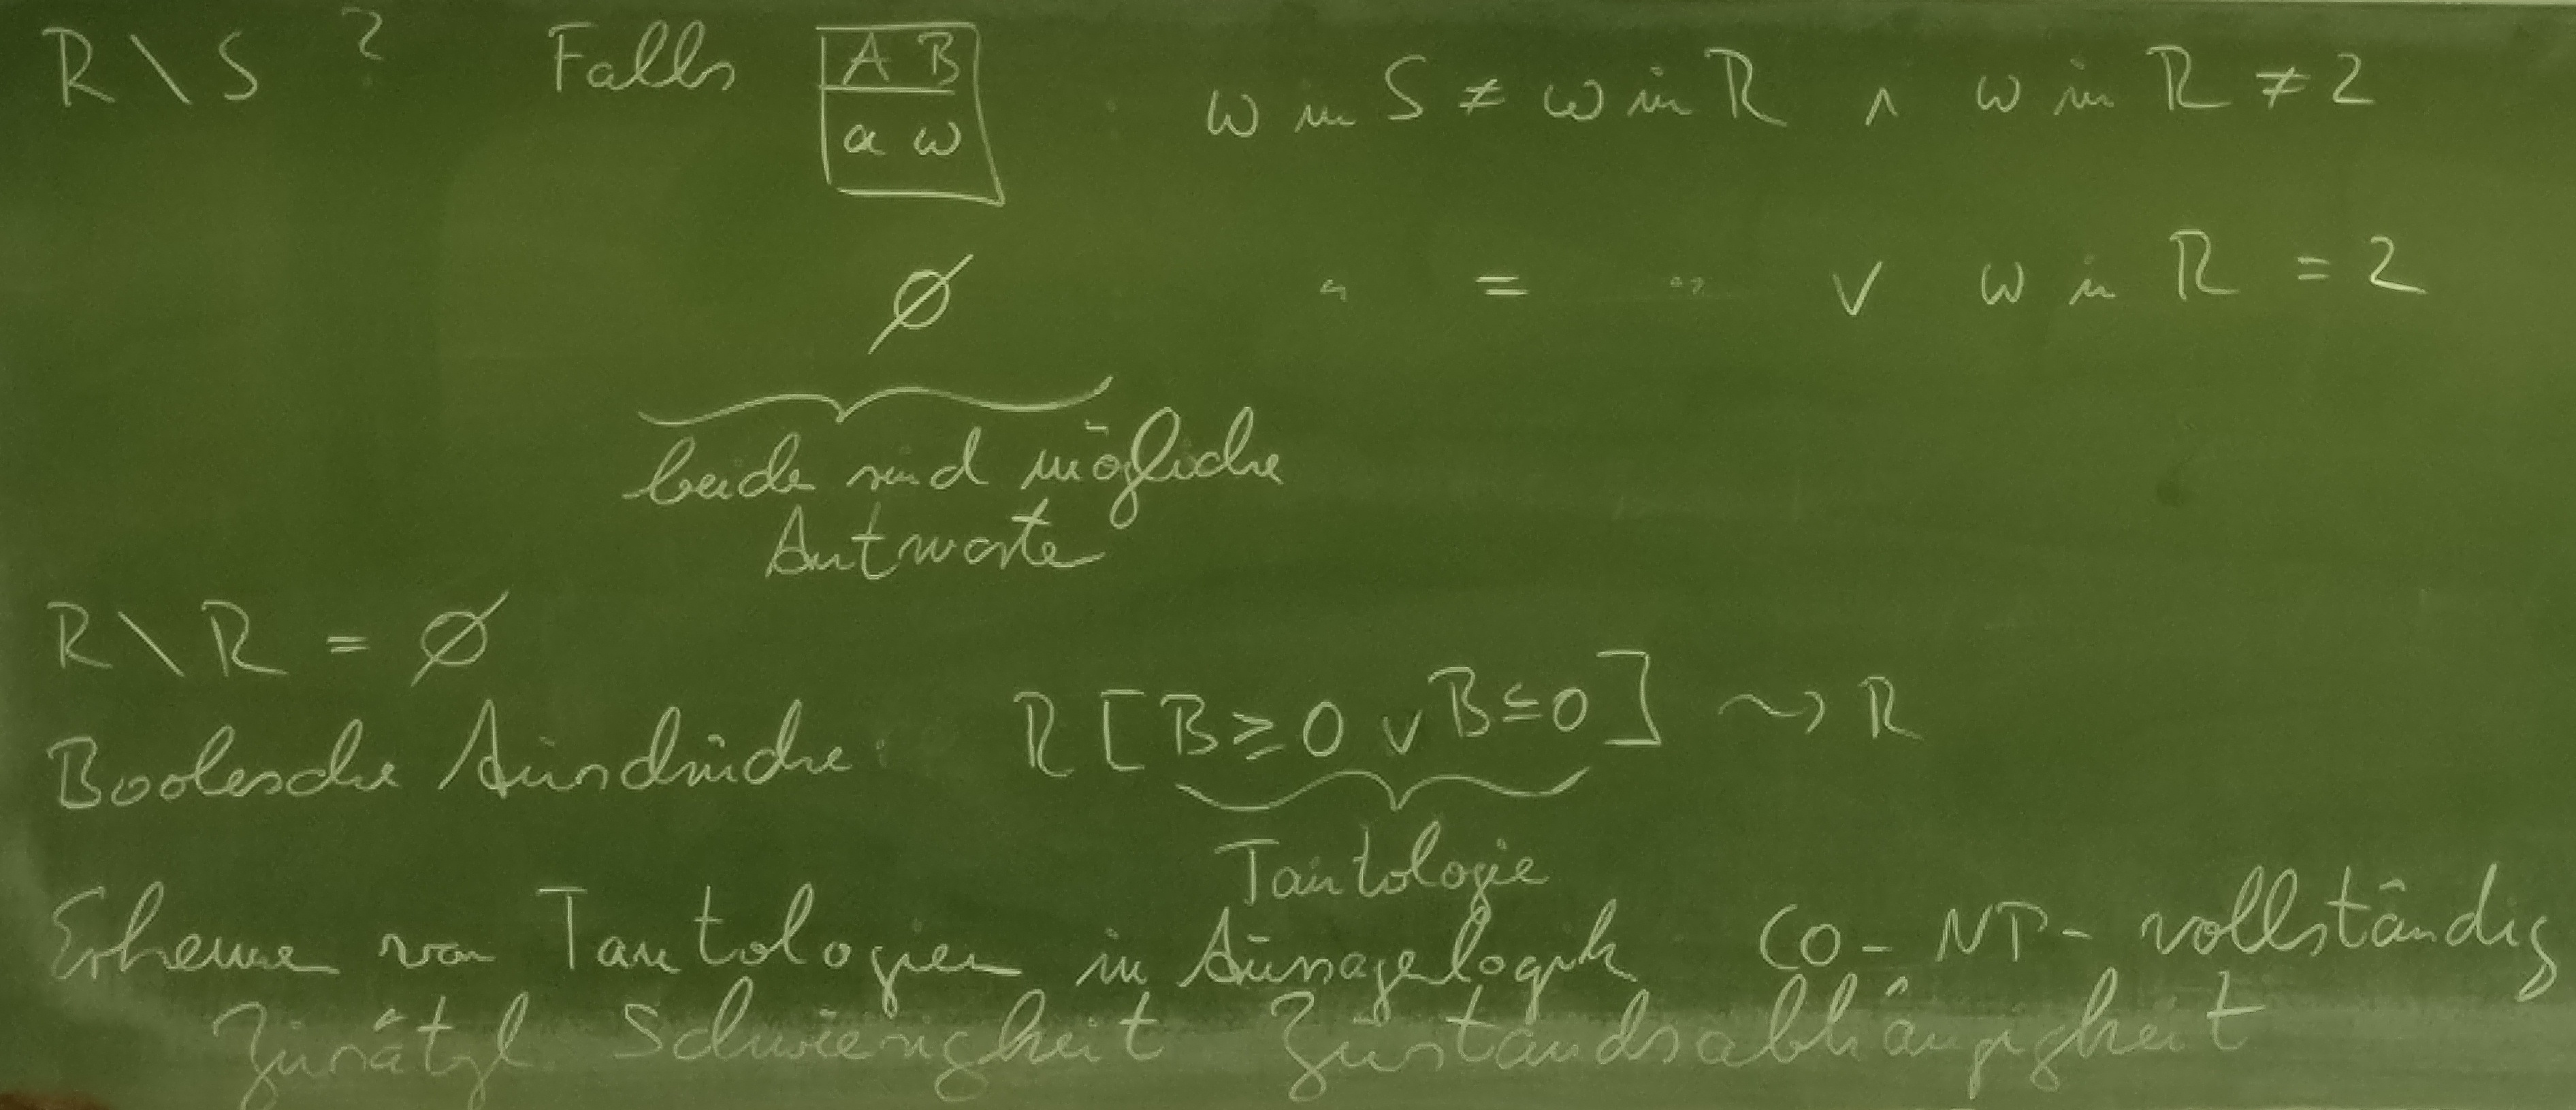
\includegraphics[width=0.7\linewidth]{img/img40}
\caption{}
\label{fig:img40}
\end{figure}

Bei Verwendung von Variablen für Vorkommen unbekannter Werte $(w_i, w_j, \cdots$ eindeutig im DB-Zustand)

Annahme $|w_i| = 1$
\begin{figure}
\centering
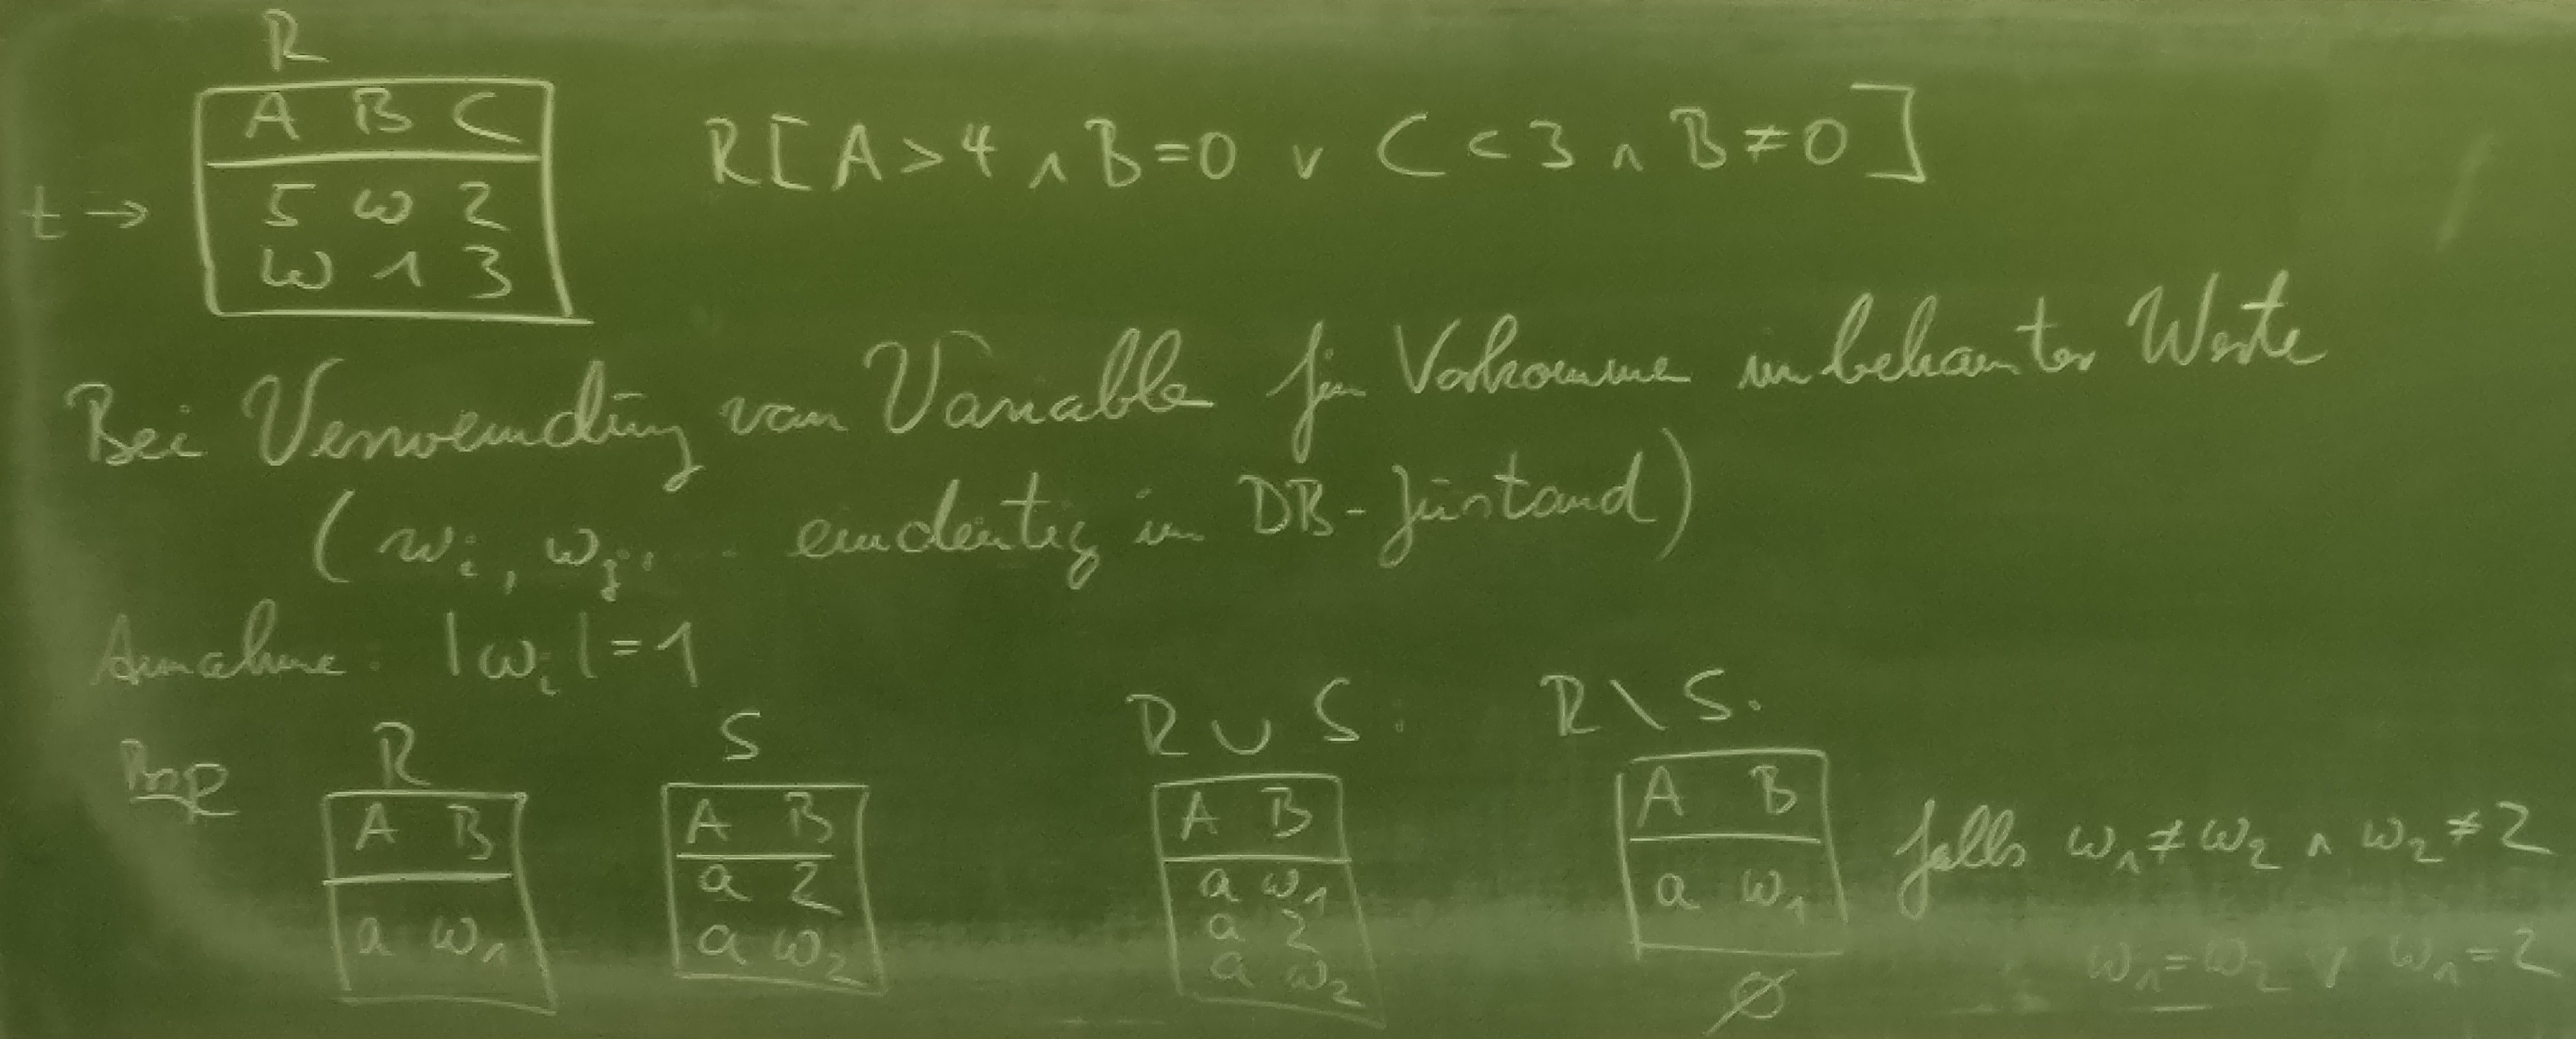
\includegraphics[width=0.7\linewidth]{img/img41}
\caption{}
\label{fig:img41}
\end{figure}
\end{document}